% options:
% thesis=B bachelor's thesis
% thesis=M master's thesis
% czech thesis in Czech language
% slovak thesis in Slovak language
% english thesis in English language
% hidelinks remove colour boxes around hyperlinks

\documentclass[thesis=B,czech]{FITthesis}[2012/06/26]

\usepackage{graphicx} %graphics files inclusion
\usepackage{dirtree} %directory tree visualisation
\usepackage{minted}
\usemintedstyle{xcode} % aby nebyly zvyrazneny chyby v Reactu, jehoz syntaxe neni znama
\usepackage{xevlna}
\usepackage{csquotes}
\usepackage{lscape}
\usepackage{bookmark} % pro moznost ukonceni part
\usepackage[style=iso-numeric]{biblatex}

\addbibresource{sources.bib}
\setcounter{biburllcpenalty}{7000} % aby se spravne lamaly adresy v bibliografii:
\setcounter{biburlucpenalty}{8000}

% % % % % % % % % % % % % % % % % % % % % % % % % % % % % % 
\department{Katedra softwarového inženýrství}
\title{Webová aplikace pro evidenci klientů projektu \enquote{Úspěšný prvňáček}}
\authorGN{Lukáš} %(křestní) jméno (jména) autora
\authorFN{Rod} %příjmení autora
\authorWithDegrees{Lukáš Rod} %jméno autora včetně současných akademických titulů
\author{Lukáš Rod} %jméno autora bez akademických titulů
\supervisor{Ing. Stanislav Kuznetsov}
\acknowledgements{Rád bych poděkoval Ing. Stanislavu Kuznetsovi za cenné rady a pomoc při tvorbě této práce. Děkuji za spolupráci své mamce, PaedDr. Janě Rodové, která se mnou jakožto lektorka Úspěšného prvňáčka po celou dobu spolupracovala. Děkuji celé své rodině a přátelům za podporu a trpělivost během celého studia.}

\abstractCS{Tato práce si klade za cíl vytvořit webovou aplikaci pro projekt \enquote{Úspěšný prvňáček}, který nabízí doučování a kurzy pro předškoláky. Výsledná aplikace má umožnit evidování klientů, jejich docházky, skupin, plateb za lekce a zobrazení celé historie klienta. Serverová část aplikace je napsána v Pythonu s webovým frameworkem Django. Klientská část je v Reactu a se serverovou částí komunikuje přes REST API díky Django REST Framework. Na závěr bylo úspěšně provedeno akceptační testování, na jehož základě proběhlo vylepšení zjištěných nedostatků. Aplikace je nasazena na hosting Heroku a lektorka ji denně používá.}

\abstractEN{The goal of this thesis is to build a web application for the project ``Successful first-grader'' which offers an extra education and courses for preschoolers. This application should allow the lector to store data about clients, their attendances, groups, payments for lectures and view the entire client's history. The server side is written in Python with Django web framework. The client side is built with React and communicates with the server REST API thanks to Django REST framework. Finally, acceptance testing was performed and all found issues were fixed. The application is deployed to Heroku hosting and is used daily by the lector.}

\placeForDeclarationOfAuthenticity{V~Praze}
\declarationOfAuthenticityOption{1} %volba Prohlášení (číslo 1-6)

\keywordsCS{webová aplikace, evidence klientů a lekcí, kurzy pro předškoláky}
\keywordsEN{web application, client and lectures management, courses for preschoolers}

\website{https://github.com/rodlukas/bachelors-thesis} %volitelná URL práce, objeví se v tiráži - úplně odstraňte, nemáte-li URL práce
%\setcounter{tocdepth}{3}
\renewcommand{\listingscaption}{Ukázka kódu}
\renewcommand{\listoflistingscaption}{Seznam ukázek kódu}
% % % % % % % % % % % % % % % % % % % % % % % % % % % % % % 

\begin{document}
    \listoflistings
    
    \begin{introduction}
    	Úspěšný prvňáček\footnote{\url{https://uspesnyprvnacek.cz/}} (dále jen ÚP) je soubor kurzů vedených speciální pedagožkou PaedDr. Janou Rodovou. Cílem kurzů je pomoci budoucímu nebo nastupujícímu prvňáčkovi rozvíjet se tak, aby byl připraven na školní docházku. Kurzy se zabývají například prevencí selhávání v oblasti čtení a psaní, správným úchopem a držením tužky, rozvojem dovedností leváka nebo prací s neklidným či hyperaktivním dítětem. Některé z kurzů využívají kromě vlastních zkušeností lektorky také revoluční metodiky např. od ruského psychologa D. B. Elkonina nebo izraelského psychologa prof. Reuvena Feuersteina, PhD., tyto metodiky se do českých končin dostávají až v posledních měsících a letech a mezi rodiči jsou především díky jasným a viditelným úspěchům v rozvoji dovedností dítěte hravou formou velmi vyhledávány.

U projektu ÚP jsem již od úplného počátku (červenec 2014), kdy mimo jiné spatřily díky mně světlo světa jeho první webové stránky. Postupem času se projekt rozšiřoval až do fáze, kdy se na základě poptávky rozrostla nabídka kurzů tak, že bylo potřeba celý web od základů předělat. Tento fakt jsem využil i k rozšíření znalostí o novinky v HTML5, CSS3 a vybudoval jsem plně responzivní stránky přesně na míru projektu.

Ruku v ruce s tímto rozšířením samozřejmě opět vzrůstal počet klientů a bylo mimo jiné potřeba přehledně evidovat klienty a lekce. Jako nejrychlejší a v danou chvíli nejjednodušší řešení byla na počátku zvolena jednoduchá tabulka v Excelu doplněná o pár barev. Díky dalšímu nárůstu klientů a zvýšenému zájmu o skupinové kurzy je ale pro lektorku velmi složité udržet evidenci jakkoliv konzistentní, praktickou a přehlednou. Nemluvě o faktu, že ji téměř nelze rozšířit o další funkcionality a rozumnou evidenci skupinových lekcí. Práce s touto tabulkou je zbytečně zdlouhavá, neefektivní, data jsou duplikována ve více souborech a také ve více formách (papír) a jakákoliv změna vyžaduje pevné nervy.

Přáním lektorky, a tedy i mým cílem, je vytvořit webovou aplikaci, která umožní evidovat klienty, jejich docházku, skupiny, platby za lekce, historii lekcí klienta a další funkcionalitu zjištěnou při analýze požadavků.

Mojí motivací pro vypracování práce na toto téma je především snaha využít technologie jako užitečný a podpůrný prvek projektu, díky kterému se jednotlivé každodenní procesy usnadní a ušetří lektorce čas. Druhou a neméně důležitou motivací je možnost prozkoumat, zmapovat a osvojit si některé z moderních technologií, ke kterým se v rámci této práce dostanu a rozšířit si tak své vědomosti a dovednosti.

V teoretické části nejprve zhodnotím aktuální stav evidence a pokusím se najít možná řešení a jejich výhody a nevýhody. Poté představím technologie, architektury a hostingy, které mohou být použity, zhodnotím je a zvolím ty vhodné pro tuto práci.

V praktické části zanalyzuji a popíši požadavky a související procesy v ÚP, navrhnu samotnou aplikaci a její části včetně struktury databáze a postupně uvedu své kroky při implementaci. Poté se budu věnovat průběhu testování včetně závěrečného akceptačního testování a provedeným úpravám. Na konec popíši nasazení výsledné aplikace na zvolený hosting a uvedu možná rozšíření v budoucnu.
    \end{introduction}
    
    \chapter{Cíle práce}
        Cílem této práce je navrhnout a implementovat webovou aplikaci, která lektorce ÚP umožní a usnadní evidenci klientů, jejich docházky, skupin,  plateb za jednotlivé lekce a také by umožnila zobrazit historii absolvovaných kurzů klientů spolu s jejich docházkou (zda chodili pravidelně apod.).

Dalším cílem, který je nutnou podmínkou pro samotnou implementaci, je analyzovat současné řešení, požadavky a související procesy v ÚP a na základě toho zvolit technologie, které budou pro tvorbu aplikace použity (databáze, jazyky, frameworky, hosting). Poté je potřeba navrhnout strukturu databáze s ohledem na požadavky.

Cílovým bodem je provedení akceptačních testů na výsledné aplikaci, příslušné úpravy a opravy zjištěných nedostatků, nasazení na hosting do běžného provozu a zhodnocení a návrh možných rozšíření v budoucnu.
    
    \part{Teoretická část}
        \chapter{Aktuální řešení}\label{aktualni-reseni}
Lektorka částečně eviduje klienty a kurzy ve svém notebooku v tabulce v programu \href{https://products.office.com/cs-cz/excel}{Microsoft Excel}, která je uložená v cloudu na \href{https://www.dropbox.com/}{Dropboxu}. Ukázka výřezu z tabulky (jména klientů jsou úmyslně skryta, jinak jsou v prvním sloupci, dále některé řádky pokračují i mimo výřez) je na obrázku \ref{fig:excel}. V prvním sloupci jsou jména a příjmení klientů a v dalších buňkách jsou pak vždy v prvním řádku datum lekce a ve druhém barevně (případně i textově další poznámky) informace o stavu termínu. Pro větší pochopení je potřeby vysvětlit jednotlivé barvy a zkratky v tabulce:
    \begin{itemize}
      \item zelená: zaplacený termín -- dále zde může být uvedeno \enquote{NT} (náhradní termín), \enquote{a} (dorazil), \enquote{placeno} (na tomto termínu došlo k zaplacení), pokud není uveden text, mělo by se jednat o předplacený termín,
      \item modrá: klient nedorazil a neomluvil se (\enquote{nepř.}) -- často je doplněno \enquote{SMS} (byla odeslána SMS klientovi, jak to s ním vypadá), nebo \enquote{oml.} (omluveno, ale pozdě, to je potřeba vědět kvůli spolehlivosti klienta),
      \item červená: nezaplacený termín -- na dané lekci potřeba platit,
      \item žlutá: omluvený termín (značeno \enquote{oml.}) -- v případě zájmu možno využít náhradní termín,
      \item fialová: termín zrušen z osobních důvodů lektorky (značeno \enquote{odv}) -- např. dovolená (\enquote{dov}).
    \end{itemize}

\begin{figure}\centering
	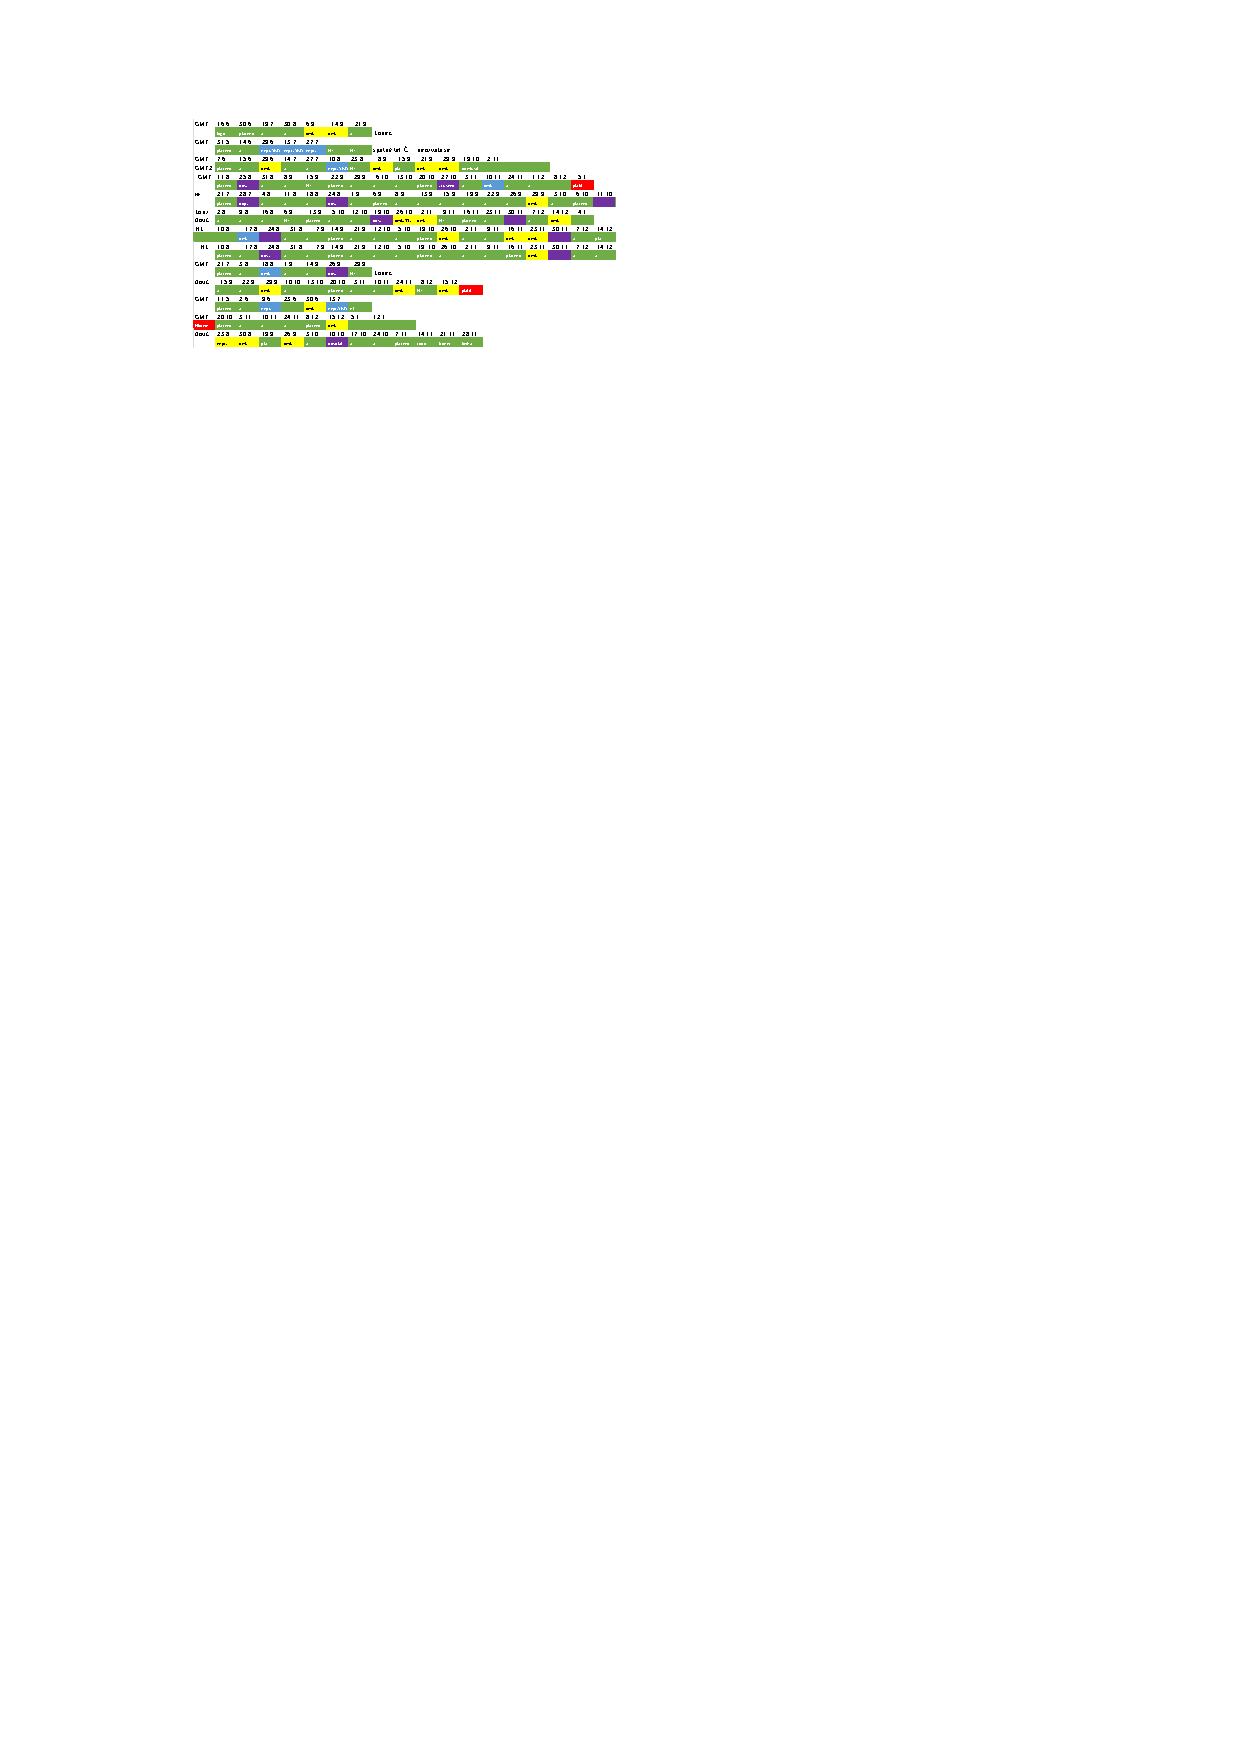
\includegraphics[width=1\textwidth]{img/excel3}
	\caption[Tabulka s evidencí klientů]{Výřez z tabulky s evidencí klientů}\label{fig:excel}
\end{figure}

Na začátku projektu to samozřejmě vypadalo jako dobrý nápad (prakticky okamžitá možnost práce bez učení) a dokud nebylo potřeba evidovat historii lekcí a kurzů a dokud bylo klientů málo, byl soubor relativně udržitelný. Po několika letech ale situace dospěla do stavu, že je třeba evidovat naráz hodně klientů (běží hodně kurzů, i těch dlouhodobějších) a přidávají se i další informace, které je potřeba evidovat, ale už to není v rámci tabulky možné. Rychlé, ale samozřejmě naprosto neudržitelné řešení, je evidování těchto údajů jinde, byla zvolena papírová forma. Tedy v tabulce jsou vedeny jednotlivé lekce, zda je zaplaceno/předplaceno, zda klient došel, omluvil se, nebo je kurz uzavřený. V papírové formě jsou poté evidovány kontakty na klienta, historie kurzů, konkrétní lekce i s časem.

Pro tuto práci je vhodné si přehledně shrnout nevýhody a výhody tohoto vedení informací. Díky tomu pak bude možné zpětně zjistit, zda nová webová aplikace všechny neduhy řeší.

    \section{Nevýhody řešení}
        \begin{itemize}
            \item \textbf{nepřehlednost:} když klient chodí dlouhodobě, musí se tabulka posouvat vpravo, ale pak nejsou vidět termíny lekcí ostatních klientů, kteří chodí kratší dobu,
            \item \textbf{nekonzistentnost:} nikdo např. nehlídá, že červená barva nutně znamená zaplatit, v souborech se často objevují chyby, lektorka omylem přepíše data jiného klienta, nemluvě o nekonzistentních textech a barvách (jiný font, velikost, zarovnání, někde napsáno \enquote{placeno} a někde pouze \enquote{pla}) apod.,
            \item neefektivní a nekomfortní práce: pokud má například klient více kurzů najednou, resp. stačí aby existoval skupinový kurz, evidence je prakticky neudržitelná a je pracné ji udržet v pořádku,
            \item \textbf{nedohledatelná historie klienta:} nelze vést přehledně historii kurzů (a příslušných lekcí) klienta: prakticky řešeno tak, že se jednou ročně v září vytvoří nový soubor, kam se překopírují pokračující klienti a připisují se noví klienti, pokud ještě navíc chodí klient na více kurzů v jednom roce, tak se musí složitě rozlišovat jednotlivé lekce,
            \item \textbf{údaje o klientovi:} neevidují se kontaktní a další informace o klientovi, řešeno papírovou evidencí,
            \item \textbf{chybí jiné pohledy:} chybí přehled pro aktuální den a týden a tato informace se nedá ani snadno dohledat, také chybí čas lekce (což se řeší papírovým diářem),
            \item \textbf{nepoužitelnost na mobilních zařízeních:} na tabletu je tabulka prakticky nespravovatelná, na mobilním zařízení ještě hůře.
        \end{itemize}
    
    \section{Výhody řešení}
        \begin{itemize}
            \item \textbf{rychlý rozjezd}: počáteční rozjezd evidence byl rychlý, nebyly potřeba žádné znalosti,
            \item \textbf{žádné poplatky}: lektorka již má Excel nainstalovaný, Dropbox je ve verzi zdarma.
        \end{itemize}
    
    \section{Shrnutí}
    Je jasné, že i přes to, že je Excel velmi silný nástroj, tak není vhodný k evidenci tohoto typu. Poskytuje sice další pokročilé funkce, díky kterým by se tato tabulka dala vylepšit, ale stále by nebyla schopna pokrýt veškeré požadavky a potřeby lektorky a také by se rozhodně nejednalo o intuitivní a jednoduchou správu (o těžkopádné editovatelnosti v mobilních zařízeních ani nemluvě).
    
\chapter{Podobné aplikace}
Po pečlivém hledání jsem nenalezl žádnou webovou aplikaci, která by pokrývala alespoň většinu požadavků. Z nalezených aplikací, které se alespoň vzdáleně podobají některým požadavkům lze jmenovat snad jen online nástroj RAYNET.cz, což je cloudový CRM (Customer Relationship Management\footnote{systém pro řízení vztahů se zákazníky pro sledování a vyhodnocování obchodních aktivit v rámci společnosti \cite{crm}}) systém pro řízení vztahů se zákazníky -- poskytuje např. databázi kontaktů, historii vztahu s klientem (schůzky, dokumenty, e-maily, reklamace, poznámky), seznam aktuálních zakázek, obchodní výsledky, kalkulace nabídek, kalendář, spolupráci kolegů, fakturaci \cite{raynet}. Jedná se o moderní, robustní systém, který sice nabízí alespoň nějakou formu evidence klientů s kalendářem a další, ale je nerozšířitelný a nesplňuje z velké části ani funkční požadavky. Funkční požadavky jsou specifické, a tak mnohem lepší než jít s kanonem na zajíce, je vyvinout webovou aplikaci na míru podle potřeb lektorky: jednoduchou, pokrývající všechny požadavky a neobsahující zbytečné funkce navíc.

\chapter{Architektonické vzory ve webových aplikacích}
Než se dostanu k samotnému hledání technologií, je potřeba pochopit, jaké architektonické vzory se ve webových aplikacích používají a proč. V této kapitole nejprve popíši dva vzory, se kterými se u různých webových technologií lze setkat. Díky tomu pak budu moci nalezené technologie v další kapitole rozlišovat i podle vzorů, na kterých jsou postaveny.

Je třeba podotknout, že tvorba (nejen) webové aplikace nutně nevyžaduje volbu jakéhokoliv architektonického vzoru, ale je dost pravděpodobné, že bez takovéto berličky bude sice možná aplikace docela fungovat, ale může být hůře rozšířitelná, spravovatelná a pochopitelná. Jakýkoliv zásah pak může vyústit v přepisování kódu celé aplikace. V tomto případě mluvím i ze své zkušenosti.

V poslední části této kapitoly popíši možné přístupy k řešení interakce mezi serverovou a klientskou částí. Díky tomuto rozdělení získám dostatečný přehled k tomu, abych mohl v další kapitole pochopit rozdílné přístupy jednotlivých technologií a rozhodnout se, které možnosti zvolit pro řešení výsledné aplikace.

    \section{MVC a další jeho varianty}\label{mvc}
    MVC (Model-view-controller) vzor původně vznikl pro desktopová GUI, ale později se rozšířil zejména mezi vývojáři webových aplikací. Mnoho populárních webových frameworků pro různé jazyky a pro serverovou i klientskou část stojí buď přímo na MVC \cite{mvc-cz1}, nebo využívají jeho odvozeninu: MVP (Model-view-presenter), MVT (Model-view-template) ad. -- souhrnně jsou někdy tyto architektury označovány jako MVW (Model-view-whatever) nebo MV* \cite{mvw}, pro odkazy na tyto technologie v dalším textu budu používat MVW.
    
    \textit{\enquote{MVC vychází z teorie, že části kódu, které vykonávají různé úkoly, by měly být od sebe oddělené.}} \cite{mvc-cz2} Nedodržení tohoto přístupu často pak může i díky absenci disciplíny programátora vést ke špagetovému kódu, vše je smícháno a výsledná aplikace je neudržitelná a těžko rozšířitelná \cite{mvc-cz2}\cite{mvc-2}. Díky tomuto rozdělení zodpovědnosti se při vývoji může programátor zaměřit pouze na příslušnou část a kód splňuje principy vysoké soudržnosti a nízké provázanosti. Na druhou stranu je ale třeba říci, že se menší aplikace při použití MVC může stát poměrně robustní, je to ale daň za dekompozici do tří částí a s tím spojené již zmíněné výhody \cite{mvc-medium1}. Další výhodou je možnost mít například více pohledů na stejný model \cite{mvc-1}.
    
    Aplikace je, jak je uvedeno v \cite{mvc-cz2}, rozdělena do tří částí: modely, pohledy a kontrolery. Pohled má na starost vykreslení stránky v HTML (Hyper Text Markup Language) a Javascriptu. Do pohledu jsou nejčastěji pomocí šablonovacího systému dodána všechna potřebná data. Modely se starají o logiku (výpočty, výsledky, získání a uložení dat, validace), při použití ORM (Object-relational mapping) korespondují modely s tabulkami v databázi. Kontroler je prostředník mezi předchozími dvěma součástmi, propojuje je a říká, co vše je potřeba provést pro výsledek. Jednoduchým příkladem znázorňujícím tento vzor je např. otevření URL \verb|http://domena.cz/uzivatele/15| -- požadavek je zachycen tzv. routerem a na základě parametrů se použije příslušný kontroler, ten zavolá model, který vyhledá daného uživatele v databázi a vrátí jeho údaje kontroleru, který vytvoří pohled a předá mu získaná data \cite{mvc-cz1}.
    
    Jak bylo již naznačeno v úvodu této kapitoly, existují mírné úpravy MVC vzoru. Tento případ lze ilustrovat na frameworku Django pro Python (podrobněji se tomuto frameworku budu věnovat v \ref{sec:python}), který využívá MVT. Dle jeho autorů \cite{django-docs-mvp} pohled nepopisuje jak data vypadají, ale která data (resp. model) na základě URL jsou zobrazena. Jak se zobrazí data je delegováno z pohledu na šablonu, která je tvořena HTML a šablonovacím jazykem. V tomto pojetí nebyl explicitně zmíněn kontroler, ten je tvořen samotným frameworkem, který odešle požadavek na příslušný pohled podle konfigurace. Zkráceně lze tedy říci, že programátor poskytne model, pohled a šablonu, které poté sváže s příslušnou URL a o zbytek se postará Django \cite{django-mvp2}.
    
    \section{CBA}\label{cba}
    V posledních letech nastal poměrně velký zlom v oblasti frameworků pro klientskou část aplikací. Vznikají nové a nové javascriptové frameworky a ty již zaběhlé se přizpůsobují poptávce a často radikálně mění své přístupy k architektuře (např. Angular, viz. \ref{sec:python}). Více a více se na straně klienta upouští od architektur MVW mj. z důvodu velmi úzké svázanosti kontroleru a pohledu a také porušování principu jedné odpovědnosti\footnote{Princip jedné odpovědnosti je jedno z pravidel objektově orientovaného programování, říká, že by každý objekt měl mít jen jednu odpovědnost (tedy jediný důvod ke změně) \cite{single-responsibility}}, protože se kontroler stará jak o logiku, tak o zpracování událostí \cite{mvc-frontend}.
    
    Vývoj vyústil ve využití v tomto odvětví doposud nepoužívané architektury CBA (Component-Based Architecture) a s tím spojených \enquote{unidirectional} architektur (tedy architektur pro jednostrannou komunikaci ke spravování stavu aplikace). Tyto dvě architektury dokážou nejen pokrýt klasický MVW přístup, ale poskytují i mnohem lepší oddělení odpovědnosti \cite{mvc-frontend}.
    
    CBA je založeno na rozdělení částí kódu na jednotlivé nezávislé, snadno testovatelné \cite{cba3}, rozšiřitelné a znovupoužitelné komponenty (v tomto případě tvořící UI), které obsahují všechny potřebné závislosti. Komponenta zapouzdřuje svou funkcionalitu a chování a zároveň navenek poskytuje jednotné rozhraní pro přístup. Díky komponentám tak může být tvorba nebo úprava UI rychleji hotová (lze používat např. i komponenty od jiných autorů) a je zajištěna konzistence napříč celou aplikací. Dalším uplatněním komponent je například jejich souvislost s procesy analýzy požadavků a návrhu během tvorby aplikace, kdy se při přidávání funkcí nemusí zdlouhavě popisovat samotná komponenta a pak teprve její rozšíření, ale stačí definovat pouze rozšiřující funkce \cite{cba1}. Použití komponent také pomáhá dodržet princip DRY (\enquote{Don't repeat yourself}) \cite{cba2}.
    
    \section{Interakce mezi serverovou a klientskou částí}\label{interakce}
    Cílem této kapitoly je ukázat aktuální možnosti řešení interakce mezi serverovou a klientskou částí. Díky tomu, že jsou weby mnohem interaktivnější než dříve, nebylo už často možné úzce svazovat klientskou a serverovou část a bylo potřeba je oddělit prostřednictvím API. To vše v této kapitole představím.
    
        \subsection{Skriptování na straně serveru}
        Webové aplikace byly typické využíváním skriptování na straně serveru \cite{moderni-webapps}, tedy na základě požadavku byl na webovém serveru připraven HTML soubor, který byl poté odeslán do klientova prohlížeče \cite{scripting-sqa} (viz. příklad Djanga na konci kapitoly \ref{mvc}). Používání tohoto způsobu samostatně se hodilo a hodí zejména pro stránky, které například přímo spolupracují s databází, vrací texty a obrázky, ale nevyžadují příliš interaktivity \cite{scripting-freecodecamp}.
        
        \subsection{Skriptování na straně klienta}\label{client-side-scripting}
        S trochou nadsázky by se, jak říká autor v \cite{scripting-freecodecamp}, dalo říci, že dnes jsou webové stránky spíše aplikace předstírající, že jsou stránky -- web je mnohem pokročilejší než dříve. Umožňuje chatování, nakupování, prohlížení aktuálního streamu novinek atd. To znamená mnohem větší zátěž na server, který vše musí obstarat. Pro pokročilejší interaktivní aplikace bylo tedy potřeba začít ve větší míře začít používat Javascript, který umožní určitou část zátěže přenést na klientskou část \cite{scripting-upwork} a skriptování na serveru doplnit o skriptování na straně klienta, tedy v prohlížeči. Je ale potřeba říci, že robustní aplikace využívající skriptování na straně klienta může být složitější implementovat, oproti těm využívající především skriptování na straně serveru \cite{scripting-fasthosts}.
        
        Vývoj dnes pokročil až do situace, že pro pokročilé možnosti interaktivity byly připraveny přímo JS frameworky \cite{scripting-upwork}, server tedy prakticky jen odešle jednoduchý HTML soubor s odkazy na Javascriptové knihovny, které obstarají zbytek práce u klienta a obsah stránky dynamicky generují a komunikují se serverem, od kterého obdrží pouze potřebné informace bez zbytečné režie navíc ve formě HTML tagů a struktury celé stránky \cite{scripting-fasthosts}. Tyto frameworky obvykle pracují s API (Application Programming Interface, viz. \ref{api}) a AJAX (Asynchronous JavaScript and XML)\footnote{technologie pro asynchronní přenos dat na pozadí bez potřeby načíst celou stránku \cite{scripting-fasthosts}} dotazy \cite{scripting-fasthosts} a představují tak jednoduchou možnost okamžité a efektivní asynchronní komunikace se serverovou částí \cite{scripting-upwork}. Podobných výsledků lze dosáhnout i bez JS frameworků a explicitně vytvořeného API, jak uvádí např. autor v \cite{scripting-simpleis}: jednotlivé pohledy s pomocí šablon na serverové straně vrací buď klasicky celou stránku a nebo pouze JSON, tyto jsou pak využity pro AJAX volání v JS na straně klienta, tento přístup se ovšem hodí pro méně interaktivní aplikace. AJAX a další operace v JS také zaznamenaly zvýšení popularity i díky knihovně \href{http://jquery.com/}{jQuery}, která přinesla značné zjednodušení práce s JS \cite{scripting-upwork}.
        
        \subsubsection{Nevýhody spojené se skriptováním na straně klienta}
        Nevýhodou skriptování na straně klienta je samozřejmě nutnost mít povolený příslušný skriptovací jazyk (tedy většinou Javascript) \cite{scripting-sqa}. Dalším potenciálním problémem může být prvotní čas načtení stránky, především JS souborů, a s tím spojený problém se SEO (Search Engine Optimization)\footnote{optimalizace nalezitelnosti na internetu \cite{seo}}, pokud není aplikace implementována korektně nebo její načtení trvá déle (roboti obdrží prázdnou stránku s načítací animací a nemusí vědět, že mají čekat na její načtení) \cite{scripting-freecodecamp}\cite{scripting-hackernoon}. Tento klasický přístup bývá obvykle nazýván jako CSR (Client-Side Rendering) a je obvykle frameworky v základu používán. Na přelomu roku 2016 a 17 se tak začaly objevovat řešení umožňující SSR (Server-Side Rendering), např. balíček \href{https://github.com/angular/universal}{Angular Universal}, mini-framework \href{https://github.com/zeit/next.js/}{next.js} pro React \cite{scripting-hackernoon}. Díky těmto dodatečným úpravám je, jak je ukázáno v \cite{scripting-ytb}, aplikace vykreslena na serveru a ve formě stringu je do výchozí kostry HTML vložen předvykreslený kód komponenty a takovýto HTML soubor je zaslán klientovi, který tak vidí bez prodlení stránku a její obsah a pouze čeká na načtení JS, aby byla stránka interaktivní, další interakce v aplikaci pak už probíhají klasicky ve stylu CSR prohlížečem. Tento přístup ale nutně nemusí znamenat zrychlení výkonu a načítání, pokud je například string, který se vygeneruje na serveru velmi dlouhý, dojde naopak ke zvýšení velikosti přenášeného HTML souboru ke klientovi a zvýšení zátěže serveru (kvůli které se na CSR přechází) a tím v důsledku použití SSR naopak ke zpomalení načítání \cite{scripting-hackernoon}. Při využití SSR je tedy potřeba brát v úvahu mnoho faktorů, mimo již zmíněných také finance a s tím související výkon serveru (server bude více zatížený a nemusí být tolik výkonný) , v úvahu také připadá kromě řešení teoretických věcí i praktické testování obou přístupů, tento přístup například zvolili vývojáři v \cite{scripting-benchmark} a po vyhodnocení výsledků pro většinu stránek zvolili SSR.
        
        Na závěr si ještě dovolím menší vsuvku k terminologii, skriptování na straně klienta a serveru je často zaměňováno za renderování a naopak (dokonce je i občas špatně interpretován smysl renderování JS na serveru \cite{scripting-chyby}), někteří autoři tyto termíny považují za stejné \cite{scripting-freecodecamp}, ale pro tuto práci je vzhledem k tomu, že se častěji opravdu používají v odlišných souvislostech, považuji za odlišné. Renderování (tedy CSR a SSR) je obvykle spojováno pouze s JS frameworky a předvykreslením stránky díky skriptování na straně serveru, kdežto skriptování na straně klienta a serveru je obecně spojováno se všemi možnými jazyky.
    
        \subsection{API}\label{api}
        Obecně uznávanou praxi při vytváření moderní webové aplikace (zejména s JS frameworkem a SPA) je zaslání úvodní stránky od serveru ke klientovi a poté načítání a ukládání dat prostřednictvím jednoduchých zpráv z klienta, neboli prostřednictvím definovaného rozhraní API \cite{api1}. 
        Poskytuje konzistentní, univerzální a flexibilní možnost sdílení dat a funkcionality napříč různými technologiemi a systémy \cite{api2}. Klient a server jsou od sebe odděleni a jsou na sobě prakticky nezávislí, změna na jedné straně (např. v databázi) by neměla vyvolat nutnost změny na straně druhé \cite{api3} -- například lze snadno vyměnit GUI (např. JS framework) a použít jiné prakticky bez nutnosti jakkoliv zasáhnout do logiky a funkcionality na serveru.
        
        Ve webových aplikacích se velmi často používá REST (Representational State Transfer) API \cite{api1}. Tato architektura podle \cite{api4} umožňuje přistupovat k datům na určitém místě (každý zdroj má jeden koncový bod, na který přistoupíme) pomocí metod HTTP (Hypertext Transfer Protocol): GET (získání dat), POST (vytvoření), PUT (úpravy celého zdroje), DELETE (smazání), PATCH (částečné úpravy) a provádět nad nimi CRUD operace. Součástí HTTP jsou i stavové kódy, na základě požadavku tak součástí odpovědi jsou dle \cite{api4} stavové kódy, například:
            \begin{itemize}
                \item \textbf{200 OK}: požadavek byl úspěšně proveden,
                \item \textbf{201 Created}: nový obsah byl vytvořen (pro POST),
                \item \textbf{400 Bad Request}: požadavek je nečitelný (např. špatný formát zaslaných dat),
                \item \textbf{401 Unauthorized}: požadavek není autorizován,
                \item \textbf{404 Not Found}: zdroj nenalezen,
                \item \textbf{405 Method Not Allowed}: zdroj není dostupný pro tuto metodu.
            \end{itemize}
        Podle \cite{api5} se REST spolu s JSON (JavaScript Object Notation) stává defacto standardem pro API webových služeb a spolu s frameworky pro vývoj aplikací na straně serveru poskytují snadnou možnost jak si vytvořit vlastní REST rozhraní. JSON je formát pro výměnu dat, který se zařadil mezi nejdůležitější formáty na webu. Jeho úspěch tkví v tom, že se s ním díky zápisu dat v souladu s JS pracuje v oblasti zápisu krátkých strukturovaných dat mnohem lépe než s konkurenčním XML (eXtensible Markup Language) \cite{api6}.
        
        \subsection{SPA a MPA}\label{spampa}
        V současné době existují dvě možnosti, jak implementovat procházení jednotlivých stránek webovou aplikací, SPA (Single-Page Application) a MPA (Multi-Page Application).
        
        MPA je podle \cite{spa1} označení pro tradiční způsob známý již od prvních webových stránek, tedy každá změna vyvolá vykreslení nové stránky v prohlížeči (tedy řečeno polopatičtěji, v otevřeném panelu se stránkou v prohlížeči se zobrazí např. načítací kolečko, dokud není přenos nové stránky ze serveru dokončen). Využívá se především pro stránky, které mají mnoho úrovní v menu, tedy jsou co se týče struktury velmi rozmanité a bohaté, dále velmi dobře fungují co se týče SEO. Nevýhodou může být úzké propojení mezi klientskou a serverovou částí. MPA nevyžaduje z podstaty věci žádné dodatečné technologie a je velmi jednoduché takovouto aplikaci vytvořit (oproti SPA).
        
        SPA je podle \cite{spa1} aplikace, která běží přímo u klienta v prohlížeči a nevyžaduje při procházení jakékoliv znovunačítání (indikované samotným prohlížečem), tento způsob používá např. Facebook, Gmail, Google Mapy ad. Díky této vlastnosti lze poskytnout uživateli vynikající UX (User Experience\footnote{celkový prožitek z používání např. webové aplikace \cite{ux}}), protože se najednou aplikace chová přirozeně a není potřeba na nic čekat a sledovat problikávání mezi stránkami při přecházení -- uživatel je stále v jednom prostoru a cítí se tak pohodlně, aplikace vlastně napodobuje desktopové programy, kde také nedochází k načítání při přechodech \cite{spa2}. Autorka v \cite{spa2} dokonce přímo píše \enquote{\textit{Nothing beats user experience offered by SPA.}} Přecházení je rychlé a většina zdrojových souborů (HTML, CSS, skripty) jsou načteny pouze na začátku a během přechodů tak dochází pouze k posílání a přijímání dat jako takových (informace z databáze apod.). Díky SPA lze jednoduše vyměnit klientskou část (která se v praxi mění častěji) při zachování stejné serverové části. Je také jednodušší znovupoužít kód serverové části pro nativní mobilní aplikaci, protože veškeré přechody mezi stránkami (kromě zaslání úvodní stránky ze serveru) jsou spravovány na straně klienta a ne serveru, jako v případě MPA. Server poskytuje pouze API, které se právě se SPA používá \cite{spa2}. Použití architektury SPA také usnadňuje tvorbu offline aplikací. Pro jednoduchou implementaci SPA se používají JS frameworky, z čehož plyne samozřejmě problém, kdy má uživatel zablokovaný JS, také je potřeba očekávat, že kód aplikace bude větší a prvotní stažení samozřejmě zabere více času (už ale víme, že je to možné vyřešit díky SSR, viz. \ref{interakce}). Pokud nastane v SPA aplikaci problém, který není korektně odchycen, může dojít ke znemožnění ovládání celé aplikace a je ji potřeba minimálně znovu načíst.

\chapter{Volba technologií}\label{technologie}
Důležitou volbou při tvorbě aplikace jsou technologie. Odvětví webových aplikací je oproti jiným specifické především svou rychlostí rozvoje. Díky tomu, že jsou webové technologie stále populárnější (například pro svou nezávislost na platformě), rostou i další požadavky programátorů a s tím ruku v ruce vzniká nepřeberné množství dalších technologií, frameworků a knihoven \cite{moderni-webapps}\cite{moderni-webapps2}. Cílem této kapitoly je poskytnout ucelený základní přehled technologií používaných v současné době pro tvorbu webových aplikací a jejich provozování a na jeho základě zvolit technologie pro tuto práci. Nejprve představím možnosti řešení na straně klienta a serveru, poté zmapuji oblast databází a srovnám hostingy pro provozování výsledné aplikace a v závěrečné části zvolím řešení pro připravovanou aplikaci ÚP.

Ještě před začátkem si dovolím jednu poznámku. Jak uvádí autoři v \cite{technologie1}, výběr technologií pouze na základě procházení článků a srovnání je velmi ošemetný a často bude programátor stát na rozcestí, kde budou proti sobě stát dvě tvrzení dvou autorů, která se budou navzájem vylučovat a občas nemusí být snadné najít bez hlubších znalostí a zkušeností to pravdivé. Při popisu technologií (a zároveň pak i výběru) tedy budu klást důraz, jak je řečeno v \cite{technologie1} a \cite{technologie2}, na účel a požadavky na aplikaci, snadnost a jednoduchost řešení (existují např. nástroje, které umožní rychlý start používání technologie, tzv. \enquote{starter boilerplates}?), ekosystém a komunita kolem dané technologie (čím více lidí, tím je pružnější vývoj, vzniká více knihoven a objeví se více otázek a odpovědí), kvalitní dokumentaci, dospělost (začínající technologie může změnit svůj směr) a také, kdo za technologií stojí.

Občas budu uvádět také data z některých průzkumů, aby bylo jasné, nakolik jsou vypovídající, uvádím zde, na jakém vzorku byly prováděny:
\begin{itemize}
    \item průzkumu Stack Overflow \cite{stack-stats17} z přelomu ledna a února 2017 se zúčastnilo přes 64 227 vývojářů z 213 zemí, z toho 70 \% zaměstnaných na plný úvazek,
    \item průzkumu Stack Overflow \cite{stack-stats17} z ledna 2018 se zúčastnilo přes 101 592 vývojářů ze 183 zemí, z toho 74 \% zaměstnaných na plný úvazek,
    \item průzkumu Jetbrains \cite{jetbrains-stats} z přelomu roku 2016 a 2017 se zúčastnilo přes 9 000 vývojářů z 20 zemí, z toho 67 \% zaměstnaných ve firmě či organizaci.
\end{itemize}

    \section{Klientská část}
    V této části popíši základní technologie, které se používají při tvorbě webových aplikací - HTML, CSS a JS. Jak už bylo zmíněno v \ref{spampa}, pro pokročilejší interakci a SPA se volí JS frameworky a knihovny, nejprve uvedu velmi dříve velmi často používanou knihovnu jQuery, poté se zaměřím přímo na aktuální frameworky a knihovny. Pochopit rozdíly v tak rychle měnícím se prostředí je náročné (frameworky mění během svých verzí i celou architekturu), informace tak snadno zastarají, stejně jako samotné aplikace. Jedním z aktuálních a velmi dobře hodnocených článků je \cite{js-fw2}, kde autor velmi rozsáhle shrnuje výhody a nevýhody jednotlivých frameworků. Cílem této práce není ale hloubková analýza všech frameworků, proto se zaměřím na jejich základní popis a výtah z některých článků, aby bylo jasné, čím se frameworky odlišují.
    
    Pro úplnost dodávám, že výčet frameworků zdaleka není úplný, z důvodů uvedených před touto částí v kapitole \ref{technologie} jsou zvoleny tři v současné době nejpopulárnější podle \cite{hot-frameworks} (seřazeno podle průměru z počtu hvězdiček na GitHub a počtu otázek na Stack Overflow). Pro představu o popularitě co se týče zájmu uživatelů při vyhledávání v Google přikládám obrázek \ref{fig:js-frameworks} aktuálního grafu s trendy (je potřeba poznamenat, že terminologie kolem verzování Angularu je mírně krkolomná, což je vidět zejména před rokem 2016, kdy existoval jen AngularJS a přesto byl Angular vyhledáván, dále \enquote{vue} je obecné slovo, široce užívané i mimo JS frameworky, z toho důvodu je zvolen jako vyhledávací dotaz \enquote{vuejs}, což mohlo mírně tomuto frameworku uškodit, je třeba tedy výsledky brát s rezervou).
    
    \begin{figure}\centering
    	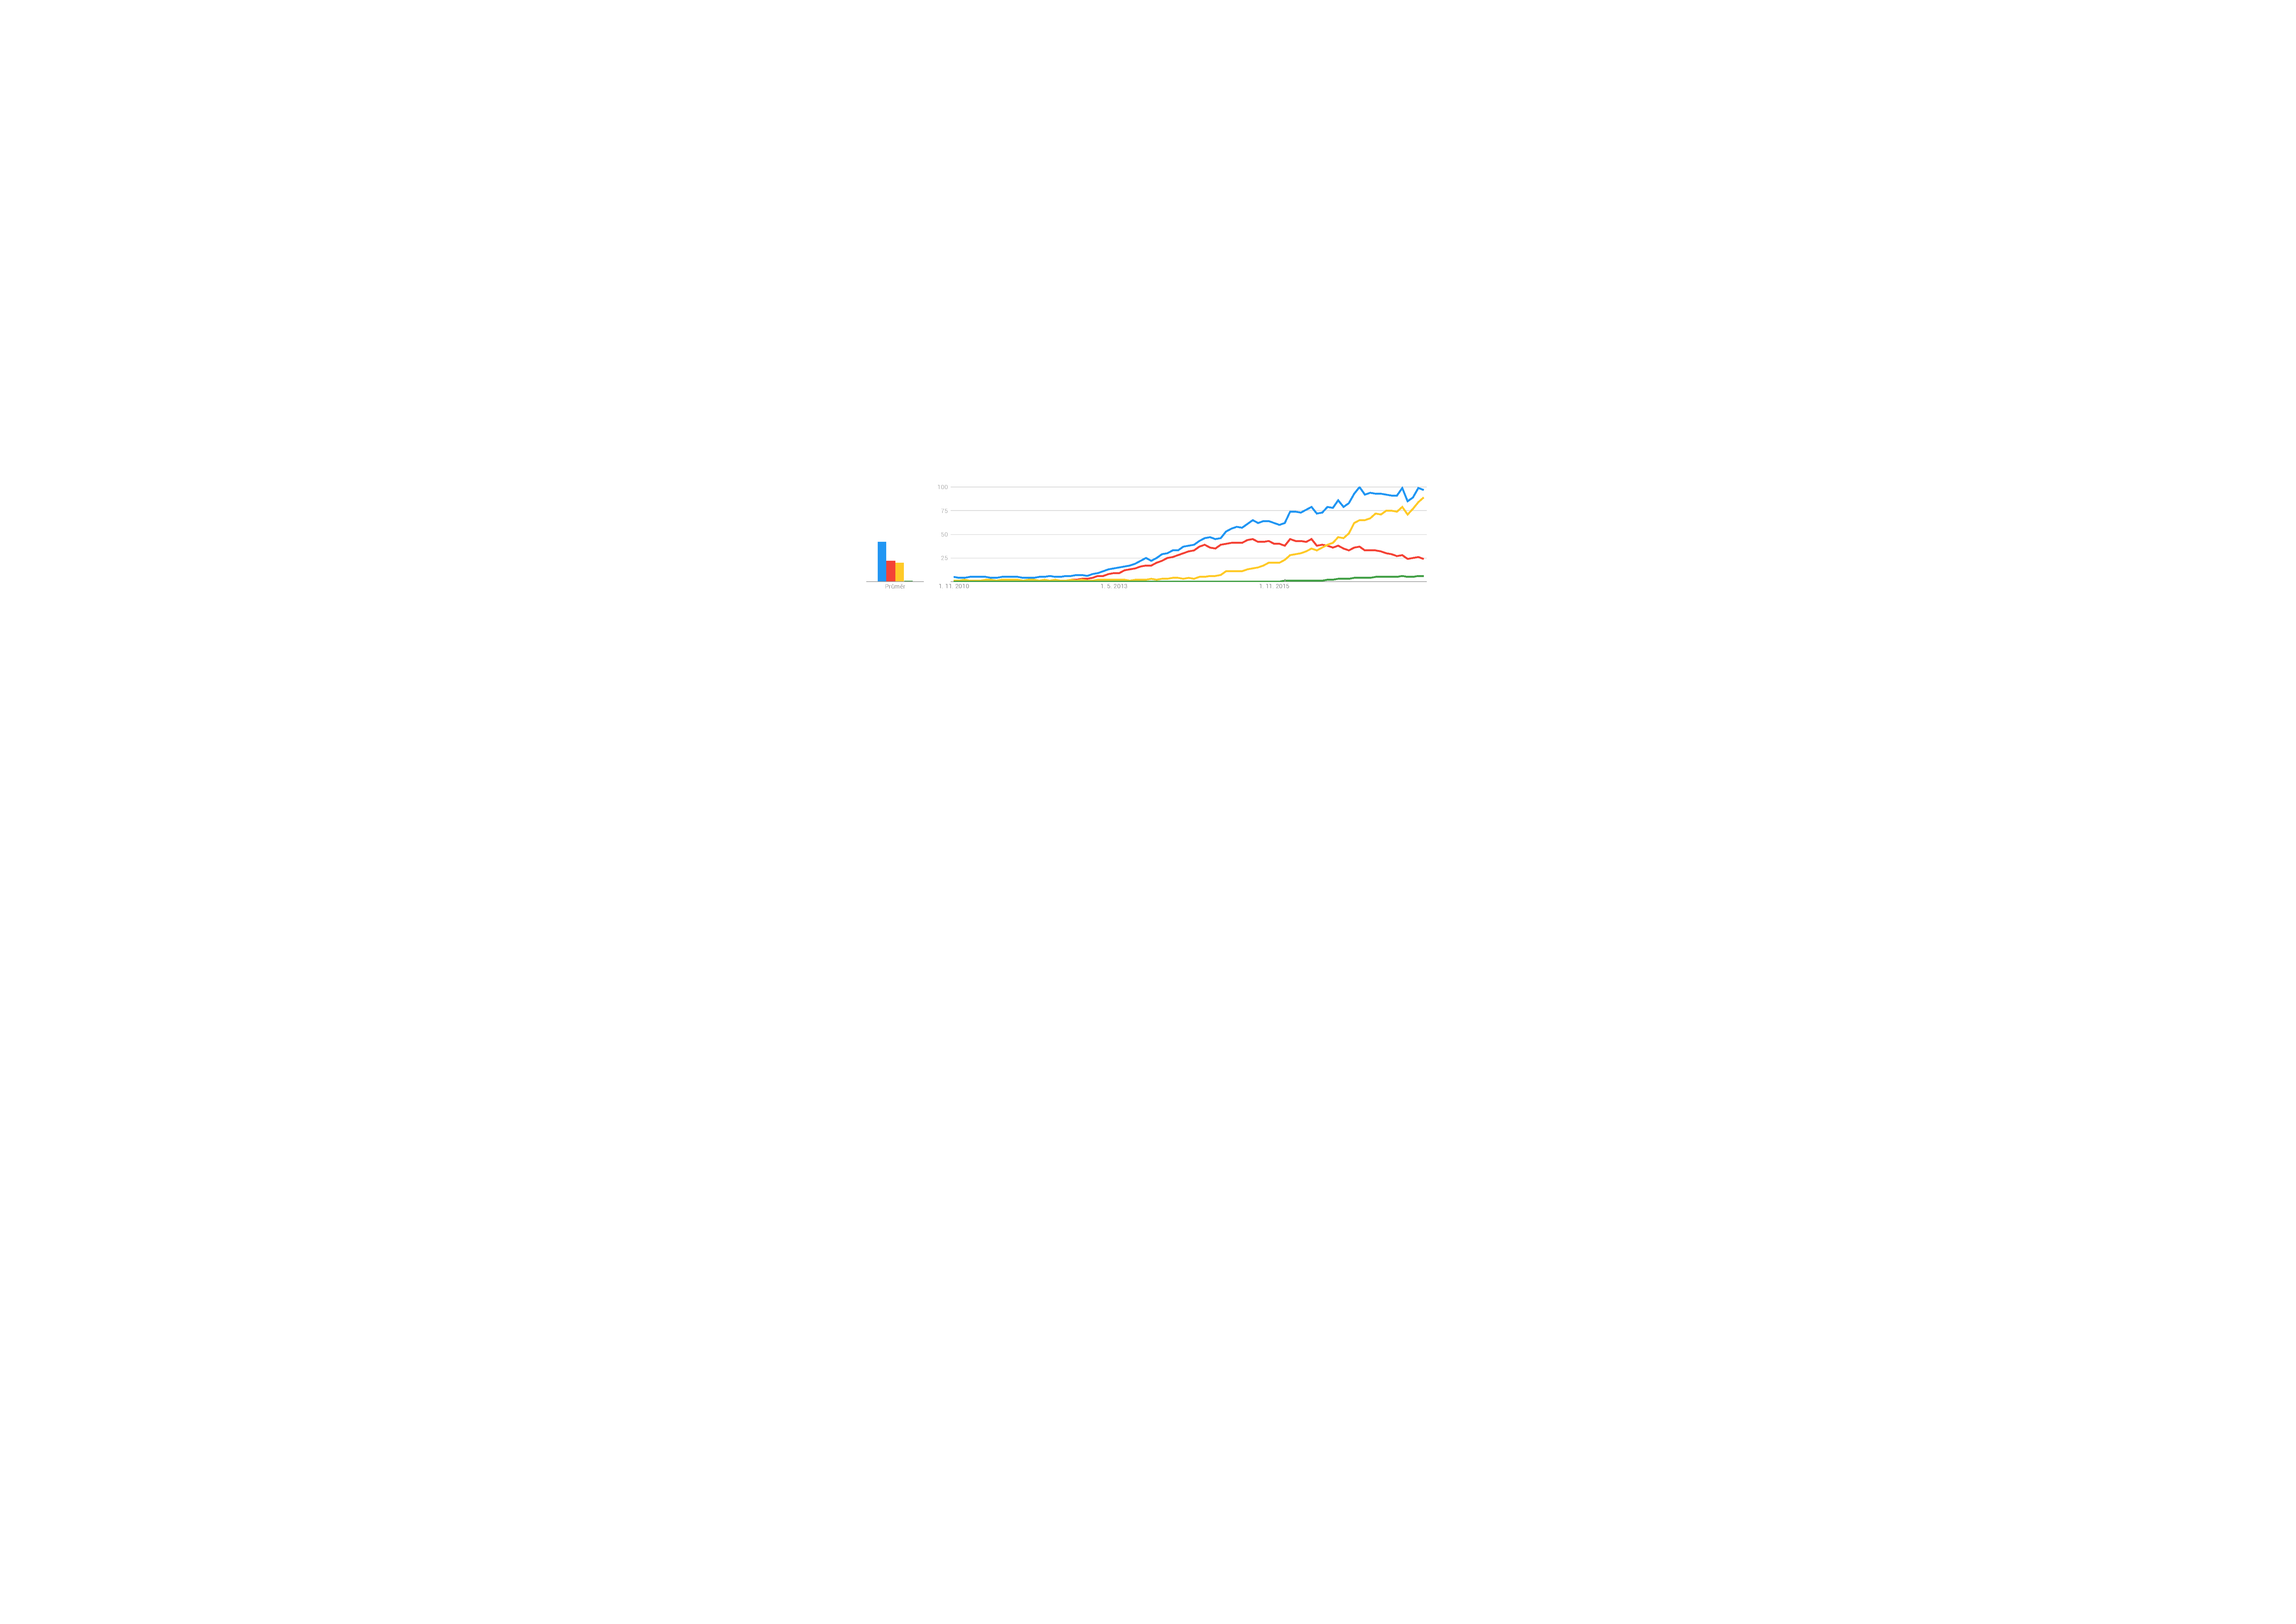
\includegraphics[width=1\textwidth]{img/js-frameworks}
    	\caption[Popularita JS frameworků ve vyhledávači Google]{Celosvětová popularita JS frameworků ve vyhledávači Google od 20. 10. 2010 do 31. 3. 2018 v kategorii Počítače a Elektronika -- modře angular, červeně angularjs, oranžově react, zeleně vuejs \cite{trends-google}}\label{fig:js-frameworks}
    \end{figure}
    
        \subsection{HTML a CSS}
        HTML (Hyper Text Markup Language) je značkovací jazyk, bez kterého se dnes při tvorbě webové aplikace nedá obejít, popisuje strukturu webové stránky pomocí HTML značek \cite{html1}. V současné době je aktuální používání HTML5, které přináší spoustu dlouho očekávaných funkcí pro moderní web \cite{html2}, je třeba ale brát na vědomí stále ještě neúplnou podporu všech novinek ze strany všech prohlížečů \cite{html3}.
        
        CSS je jazyk pro zápis způsobu zobrazení elementů HTML stránky \cite{css2}. V současné době se používá CSS3, které přineslo mj. možnost jednoduše vytvářet responsivní stránky, animace a přechody \cite{css3}. Stejně jako u HTML5 je třeba brát v úvahu neúplnou podporu všech novinek ze strany všech prohlížečů \cite{css1}.
        
        \subsection{Javascript, jQuery}\label{js}
        Javascript je skriptovací interpretovaný jazyk, který se obvykle používá pro skriptování na straně klienta (na straně serveru viz. \ref{nodejs}) -- pro jakoukoliv interakci a animace na stránce \cite{js2}. Během let se stala mezi programátory velmi populární knihovna jQuery (padla o ní řeč už v \ref{client-side-scripting}), která výrazně zjednodušuje a zaobaluje syntaxi JS \cite{scripting-upwork}. Je to nejpoužívanější skriptovací jazyk vycházející ze specifikací ECMAScript, v posledních letech díky implementaci specifikací ECMAScript 5, 5.1, 6, 7 a 8 obdržel spoustu důležitých funkcionalit a syntaktické nadstavby včetně tříd \cite{js3}. Opět je zde samozřejmě problém s kompatibilitou v prohlížečích, to se ale obvykle řeší použitím transpileru (překladač mezi dvěma jazyky na stejné úrovni abstrakce) Babel, který může kromě transpilace poskytnout i polyfilly (nahrazují nativní API prohlížeče) \cite{js4} \cite{js1}. Další často používanou nadstavbou pro větší JS aplikace jsou jazyky jako TypeScript, CoffeeScript \cite{js5} nebo rozšíření JSX (aby HTML v JS vypadalo jako HTML, ačkoliv se jedná o prosté JS funkce \cite{js-fw3}) \cite{js6}.
        
        \subsection{Angular, AngularJS}\label{sec:angular}
        Angular a AngularJS jsou JS frameworky od společnosti Google. AngularJS byl vytvořen v roce 2009 a stavěl na technologii MVC. Postupem času se ale začalo ukazovat, že je potřeba použít spíše CBA (viz. \ref{cba}) a změnit přístup i v jiných oblastech. \cite{angular1}
        
        V roce 2016 byl tak vydán Angular, později nazývaný Angular 2, vzhledem ke zpětné nekompatibilitě a mnoha změnám i v dalších verzích \cite{js-fw2} se to z některých stran nesetkalo s kladným přijetím \cite{angular2}\cite{js-fw1}. Nabízí bohatou knihovnu včetně API pro HTTP požadavky ad., používá Typescript (o kterém jsem psal v předchozím odstavci \ref{js}).
        
        \subsection{React}\label{react}
        React je podle \cite{react} knihovna (ne framework, viz. další rozebrání v \cite{js-fw1}) od Facebooku, která umožňuje budovat interaktivní uživatelská prostředí. Oproti Angularu je React velmi jednoduchý a malý, protože neobsahuje prakticky žádné dodatečné funkce, v tom spoléhá na komunitu \cite{js-fw1}, je potřeba si tedy uvědomit, že i pro HTTP požadavky je zde potřeba najít a zvolit vhodnou knihovnu, jinak lze použít pouze běžné JS požadavky. Pro tvorbu HTML lze volitelně použít JSX (viz. \ref{js}), je to výhodné zejména z důvodu jednoduššího a přehlednějšího zápisu.
        
        \subsection{VueJS}
        VueJS by se s trochou nadsázky dal označit za kombinaci Angularu a Reactu \cite{js-fw5}, z obou přináší skvělé věci a je velmi kladně hodnocen lidmi, kteří před ním pracovali s AngularJS nebo Reactem \cite{js-fw1}. Nevýhodou je zatím jeho menší rozšířenost a používanost \cite{js-fw1} a také fakt, že za ním nestojí firma, ale jednotlivec, i z toho důvodu jsou zatím ze strany firem zatím upřednostňovány React a Angular \cite{js-fw4}, jeho popularita se ale pomalu zvyšuje a objevují se týmy, které ho na své větší projekty reálně používají \cite{js-fw1}.
    
    
    \section{Serverová část}
    Volba programovacího jazyka pro serverovou část jde často ruku v ruce s volbou frameworku. Cílem této části je uvést nejpoužívanější řešení pro webové aplikace včetně možností frameworků. Pro úplnost opět dodávám, že výčet technologií není úplný, podrobněji se nezaobírám např. jazyky C++, Go, Perl a příslušnými frameworky, a to především buď z důvodu velmi specifických možností využití \cite{technologie-c++} nebo menší rozšířenosti \cite{stack-stats18}\cite{jetbrains-stats}. Ze stejných důvodů také volím pouze nejpopulárnější frameworky podle \cite{hot-frameworks}.
    
    \begin{figure}\centering
    	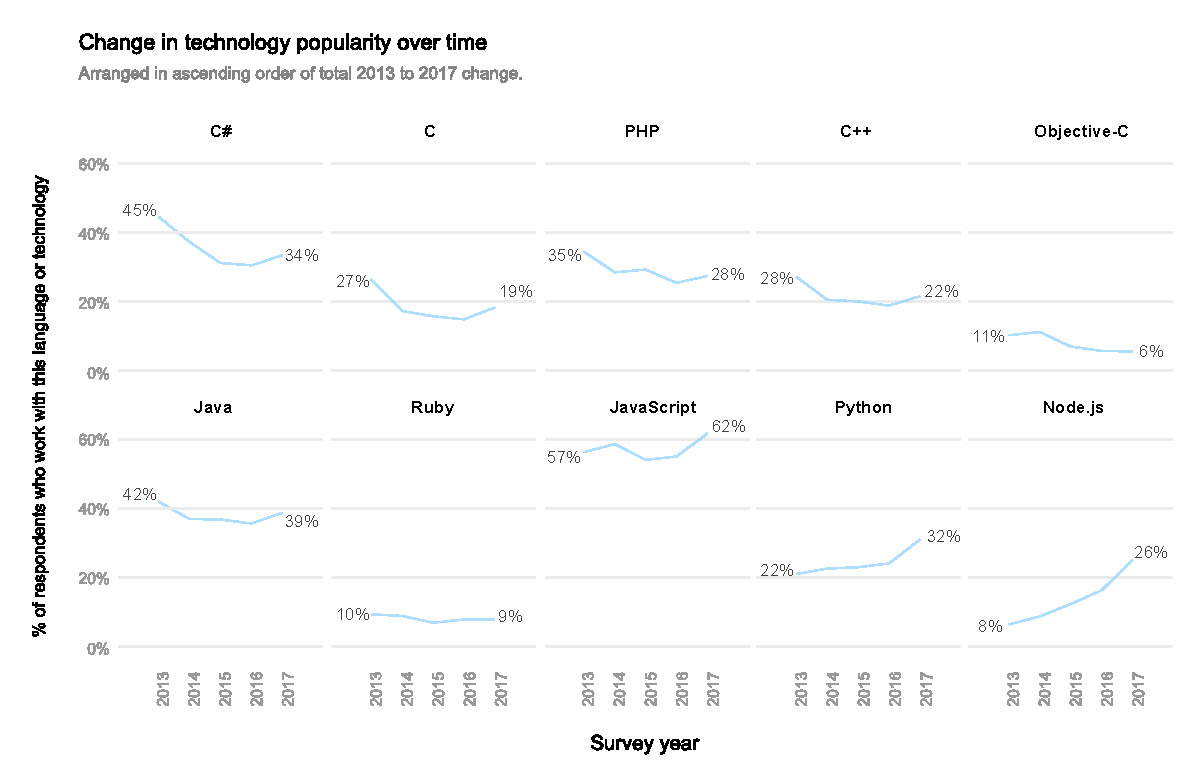
\includegraphics[width=1\textwidth]{img/stack-stats}
    	\caption[Popularita technologií mezi lety 2013 a 2017 dle průzkumu Stack Overflow]{Popularita technologií mezi lety 2013 a 2017 dle průzkumu Stack Overflow \cite{stack-stats17}}\label{fig:stack-stats17}
    \end{figure}
    
        \subsection{PHP}
        PHP je slabě typovaný jazyk, který se obvykle používá pouze ve světě webu \cite{tech-python1}. Podle \cite{tech-php1} jej využívá přes 80 \% webů, díky této popularitě tak programátoři mají také k dispozici nepřeberné množství hostingů (oproti ostatním jazykům), které jsou levné, nebo dokonce zdarma \cite{tech-python4} (např. velmi populární tuzemský hosting Endora\footnote{\url{https://www.endora.cz/}}). Hlavní výhodou je, že je v něm velmi jednoduché začít tvořit webovou aplikaci i bez frameworku, to je ale i hlavní nevýhoda, protože mnoho programátorů pak píše špagetový kód a aplikace jsou téměř neudržovatelné \cite{tech-php2}. Dalším argumentem pro využití PHP může také být, že nejpopulárnější CMS (Content Management System) Wordpress běží na PHP \cite{tech-python2}. I z těchto důvodů se často dle \cite{tech1} používají frameworky, kterých je oproti jiným jazykům pro PHP mnohem více, např. Laravel, Zend, Symfony a také tuzemský Nette. Často zmiňovanými nevýhodami jsou např. poměrně nezorganizovaná standardní knihovna \cite{tech-python1}, názvosloví funkcí a nepohodlná práce při použití UTF-8 \cite{tech-php3}.
        
        \subsection{Java}
        Java je jazyk obecně používaný jak pro webové, mobilní, tak desktopové aplikace, často se používá pro rozsáhlé podnikové systémy díky bezpečnosti a výkonu \cite{tech2}. Pro webové aplikace nabízí mnoho nástrojů a frameworků, např. Spring MVC, Play, JSF, Google Web Toolkit ad. Je třeba vyzdvihnout framework Play, který umožňuje stavět jednoduché aplikace v jazycích Java nebo Scala a je vhodný i menší projekty (oproti některým jiným frameworkům \cite{tech-java1}) \cite{tech-java2}. Dle \cite{tech-php1} je Java třetí nejpoužívanější technologie na straně serveru.
        
        \subsection{C\#}
        C\# je jazyk s širokým použitím pro vytváření bezpečných a robustních aplikací, aplikace (a dále zmiňované frameworky) pak běží na platformě .NET Framework na Windows nebo na multiplatformním .NET Core \cite{tech-csharp1}. V roce 2016 Microsoft vydal nový moderní framework ASP.NET Core, který spojuje starší frameworky ASP.NET MVC a ASP.NET Web API \cite{tech-csharp1}. I díky robustnosti celého prostředí se často používá v korporátním prostředí \cite{tech-csharp3}. Dle \cite{tech-php1} je ASP.NET druhá nejpoužívanější technologie na straně serveru.
        
        \subsection{Ruby}
        Ruby je jazyk se zajímavou a jednoduchou syntaxí a silným objektovým založením \cite{tech-ruby1}.
        Používá se ve spojení s frameworkem Ruby on Rails, díky kterému je velmi jednoduché začít po chvíli programování vidět výsledky \cite{tech1}. Práce s frameworkem je postavena na mnoha návrhových vzorech a konvencích, což někteří považují za výhodu \cite{tech1} a jiní za nevýhodu \cite{tech-ruby2}.
        
        \subsection{Python}\label{sec:python}
        Python je silně typovaný jazyk, vyniká především svou jednoduchou syntaxí a srozumitelnou standardní knihovnou s dobrou organizací \cite{tech-python1}, jedná se o obecný jazyk a díky dostupnosti velkého množství knihoven, např. pro strojové učení a umělou inteligenci a je tak velmi populární volbou v těchto odvětvích \cite{tech-python3}. Zatím poslední verzí je verze 3, která je záměrně zpětně nekompatibilní s verzí 2 -- dle autora jazyka je cílem napravit hříchy jazyka z minulosti \cite{tech-python6}. Jak je vidět na obrázku \ref{fig:stack-stats17}, jeho popularita se stále zvyšuje.
        
        Python se původně se pro webové aplikace vůbec nepoužíval, pro jednoduché vytvoření webové aplikace je potřeba použít některý z webových frameworků, nejpopulárnější je Django a Flask \cite{tech-python4}. Podle \cite{tech-python5} lze tyto dva frameworky od sebe poměrně snadno rozlišit: Flask je jednoduchý, modulární framework a je na uživateli, jaké součástí si do něj přidá, naproti tomu Django je tzv. \enquote{batteries included} framework, tedy má v sobě spoustu nástrojů, díky kterým může uživatel rychle vyvíjet webovou aplikaci bez řešení, který modul zvolit.
        
        \subsection{Node.js}\label{nodejs}
        Node.js je prostředí pro spouštění pro efektivní běh JS na straně serveru, díky JS hojně využívá model událostí a asynchronních operací pro maximalizaci výkonu a minimalizaci režie procesoru. Ideou autorů bylo sjednocení jazyka serverové a klientské části, protože moderní aplikace obvykle stály na použití JS na klientovi, ale ne na serveru. \cite{tech1}
        
        Popularita Node.js, jak je vidět na obrázku \ref{fig:stack-stats17}, strmě roste, na druhou stranu se ale objevují názory \cite{tech-node1}, že JS patří pouze na stranu klienta. Pro jednodušší vývoj webových aplikací se často používá framework Express \cite{tech-node2}. I když programátor zvolí na server jinou technologii, často se i tak s Node.js setká např. ve formě nejpoužívanějšího správce balíčků pro JS s názvem npm, který je na Node.js postaven \cite{tech1}.


    \section{Databáze}
    Vzhledem k tomu, že volba databáze je často úzce svázaná jak s použitými technologiemi, tak s dostupnými technologiemi na straně hostingu, a také k tomu, že zde není prostor pro testování, zda se hodí více MySQL nebo PostgreSQL na základě benchmarků apod., rozhodl jsem se pouze krátce uvést možnosti řešení databází v dnešní době. V průzkumu Stack Overflow \cite{stack-stats18} je vidět na obrázku \ref{fig:stack-stats18-db} šest nejpopulárnějších databázových řešení v tomto roce.
    
    \begin{figure}\centering
    	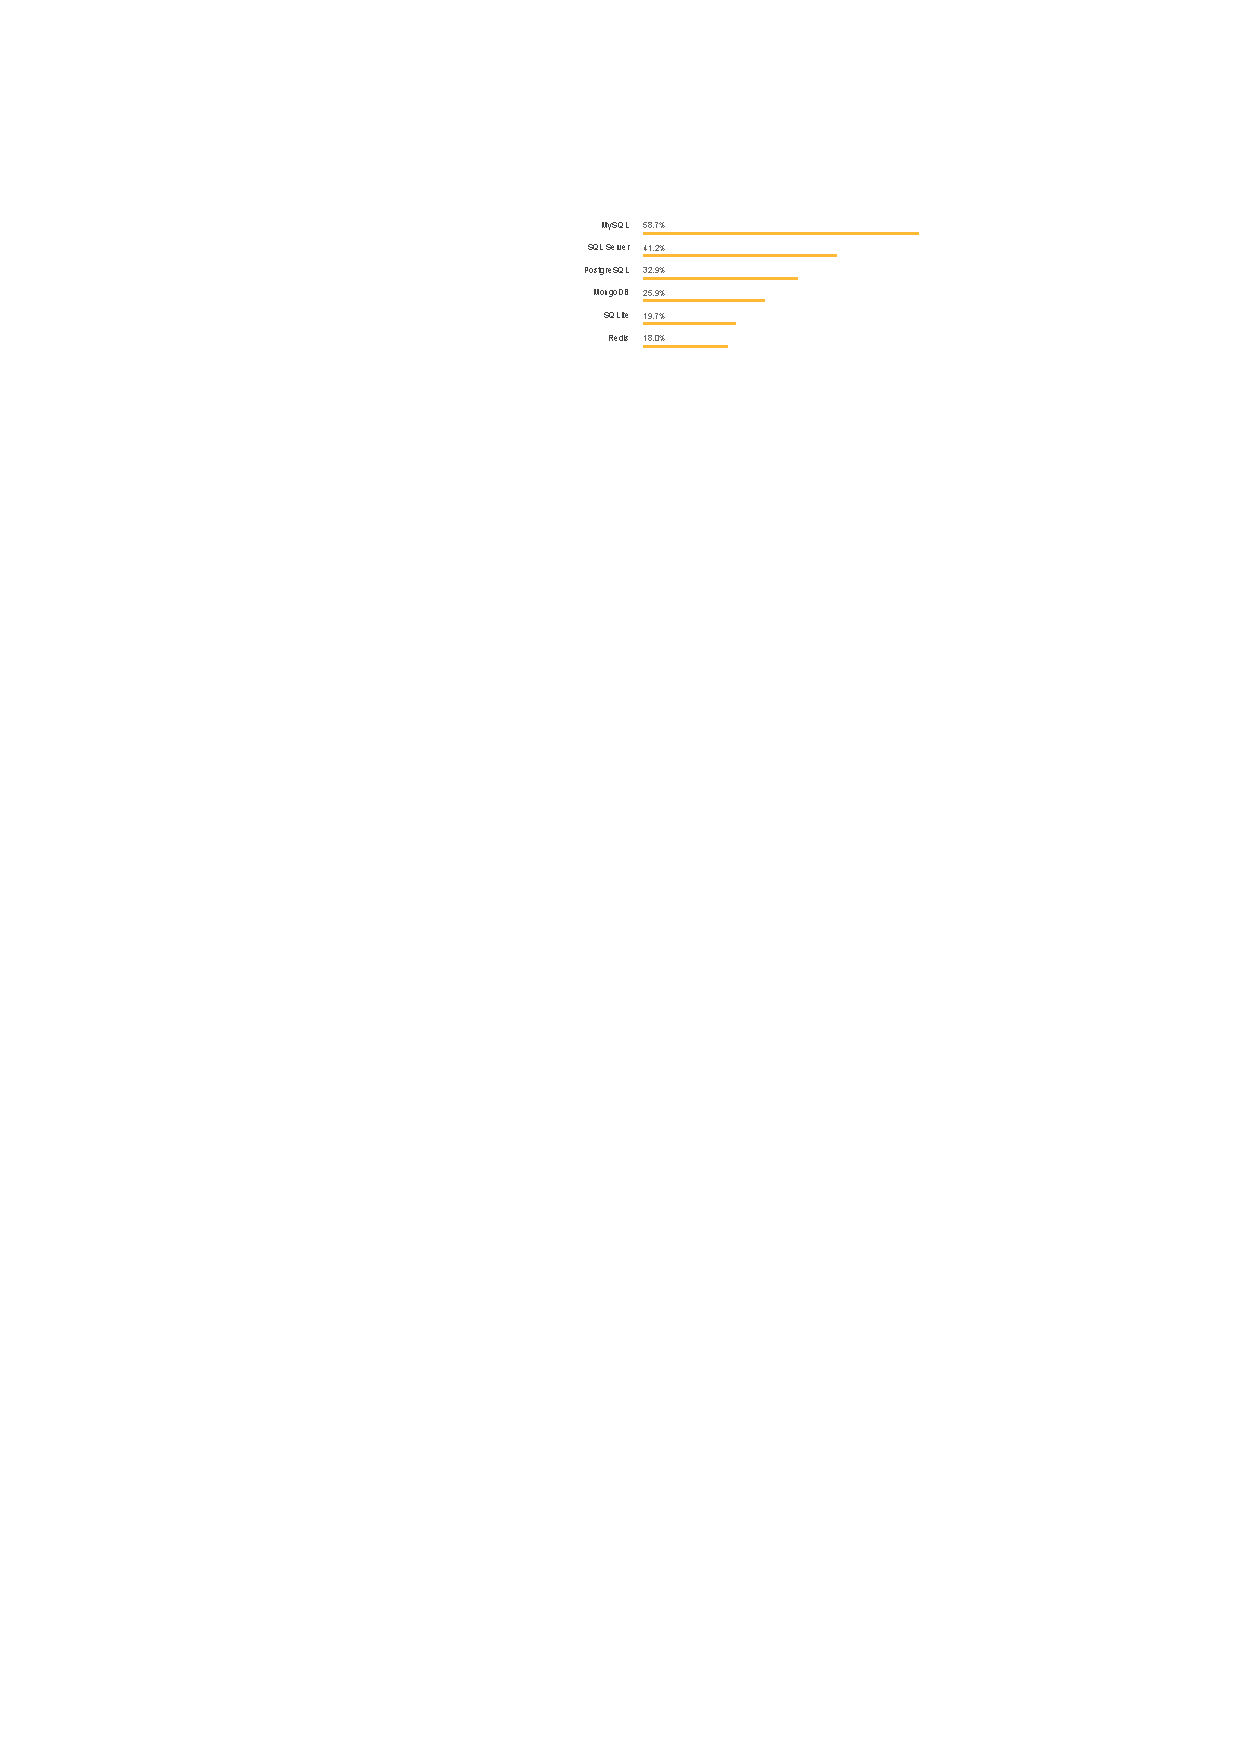
\includegraphics[width=0.9\textwidth]{img/stack-stats-db}
    	\caption[Popularita databází v roce 2018 dle průzkumu Stack Overflow]{Šest nejpopulárnějších databází v roce 2018 dle průzkumu Stack Overflow \cite{stack-stats18}}\label{fig:stack-stats18-db}
    \end{figure}
    
    Krátce si jednotlivé databáze popišme. MySQL \cite{db1}, SQLite \cite{db2} (která je velmi jednoduchá a často se např. používá pro prototypy aplikací) a SQL Server jsou relační databáze, PostgreSQL \cite{db3} je objektově relační databáze, všechny tedy sdílí tradiční práci s SQL (Structured Query Language). MongoDB \cite{db4} a Redis \cite{db5} jsou naproti tomu NoSQL databáze, jsou to moderní, flexibilní a škálovatelná řešení často se uplatňující v transakčně náročných aplikacích díky své rychlost. MongoDB je dokumentová databáze a Redis databáze založená na formátu klíč--hodnota a na využívání mezipaměti.
    
    
    \section{Srovnání hostingů}
    Je důležité rozlišit si jednotlivé typy hostingů, kde může být aplikace uložena, pro tuto práci jsou možné 3 způsoby: tradiční hosting, PaaS a IaaS.
    
    Tradiční hosting je velmi populární hlavně díky své cenové dostupnosti a rozšířenosti, na serveru, který má nějakou konfiguraci, systém a komponenty, je každému uživateli vyhrazen jeho prostor \cite{hosting2}, často je nabízena funkcionalita emailů ad.
    
    PaaS (Platform as a service) a IaaS (Infrastructure as a Service) jsou podle \cite{hosting1} cloudové služby, které se od sebe liší mírou toho, co umožní uživateli, a co dělají za něj, společné mají to, že poskytnou uživateli virtuální prostředí. IaaS je prakticky pronájem hardwaru na dálku, nabízí zákazníkům plnou kontrolu nad vším od systému až po databází a aplikace. PaaS je v tomto ohledu striktnější a od poskytovatele dostanou uživatelé předpřipravené prostředí s mnoha doplněnými funkcemi včetně propojení s verzovacími systémy, mohou si vybrat konkrétní databázi a jazyk, ale nemají přístup k samotnému systému a dalším funkcím, díky tomu se můžou ale zaměřit na samotný vývoj aplikace, testování a nasazování.
    
        \subsection{Heroku}\label{heroku}
        Heroku od firmy Salesforce.com je PaaS služba, která podle \cite{heroku1} podporuje jazyky Ruby, PHP, Go, Python, Java, Scala, Clojure, technologii Node.js a jako výchozí databáze nabízí PostgreSQL a také Redis. Poskytují několik programů, včetně jednoho zdarma \cite{heroku2}, ten má samozřejmě několik omezení:
            \begin{itemize}
                \item po 30 minutách neaktivity aplikace usíná a chvíli trvá, než se probudí,
                \item je k dispozici až 1000 hodin provozu měsíčně pro jeden účet (což není žádný problém, protože v rámci účtu neběží žádné další aplikace, navíc 1000 hodin je v přepočtu přes 41 dnů provozu na měsíc) a
                \item posledním omezením je maximálně 10 000 řádků v databázi PostgreSQL (rozšíření na 10 milionů stojí 9 \$ měsíčně)
            \end{itemize}
        Výhodou Heroku je, že i v programu zdarma dává možnost vybrat servery v Evropě \cite{heroku3}, také nabízí velkou škálu předpřipravených doplňků, díky kterým je možné aplikaci rozšířit o další funkcionalitu. Pokud by byl potřeba pokročilejší program mj. bez usínání aplikace, příplatek činí dalších 7 \$ měsíčně.
        
        \subsection{DigitalOcean}
        DigitalOcean je podle \cite{digitalocean1} služba IaaS, mj. poskytuje distribuce Ubuntu, CentOS, Debian, Fedora, CoreOS a FreeBSD. Obsahuje spoustu předpřipravených možností a návodů, které usnadní start aplikace v typických prostředích. Servery má mj. i v Evropě \cite{digitalocean2}. Nejlevnější řešení stojí podle \cite{digitalocean3}.
        
        \subsection{Openshift}
        Openshift od firmy Red Hat je služba PaaS, která podle \cite{openshift1} umožňuje hostovat projekty v jazycích Java, Python, Perl, Ruby, PHP, technologiích .NET Core, Node.js na serverech Apache a Tomcat. Co se týče databází, nabízí MySQL, PostgreSQL, Redis, MariaDB a MongoDB. Má dva programy \cite{openshift2}, zdarma nabízí hostování projektu, které je především limitováno tím, že po 30 minutách neaktivity je aplikace uspána, její probuzení chvíli trvá a zároveň musí spát alespoň 18 hodin v každém ze 72hodinových intervalů. Další nevýhodou verze zdarma jsou servery umístěné v Severní Americe, ty evropské jsou pouze v placené variantě, která stojí 50 \$.
        
        \subsection{PythonAnyWhere}
        PythonAnyWhere je podle \cite{pythonanywhere1} a \cite{pythonanywhere2} Paas nabízející hosting pro aplikace v Pythonu -- zdarma umožňuje provozovat aplikace s omezeným výkonem a MySQL databází, vyšší výkon včetně dalších možností (např. Postgres) lze získat za příplatek 5 \$ nebo více. Servery má v USA \cite{pythonanywhere3}.
        
        \subsection{Další možnosti}
        Dalšími možnostmi jsou například PaaS služba Google App Engine \cite{googleapp} a IaaS služba od Amazon Web Services s názvem EC2 \cite{aws1}, obě mají velmi objemné ceníky se spoustou pokročilých variant včetně kalkulátorů a není lehké se v nich vyznat (například AWS dává k dispozici 12 měsíců s určitými podmínkami zdarma, ale při jejich překročení nebo vypršení roční lhůty přesune uživatele do placeného programu bez možnosti návratu \cite{aws2}). Také je potřeba zmínit český hosting Roští, který podle \cite{rosti} nabízí hosting aplikací v Pythonu, Ruby, PHP a Node.js, nabízí relativně levný program za 99 Kč měsíčně. Vzhledem k tomu, že už jsem našel rozumné varianty (dokonce i zdarma), které pro rozjezd projektu postačí, nebudu se těmito službami hlouběji v této práci zaobírat.

    \section{Zvolené řešení}\label{reseni}
    Na úvod bych chtěl krátce uvést své zkušenosti s technologiemi v oblasti webových aplikaci. Vyzkoušel jsem si v minulosti práci s Javou a Servlety a také čistým PHP, nikdy jsem tedy nepracoval s frameworky a na základě těchto zkušeností jsem chtěl zvolit nějaký framework. Co se týče klientské části, zde jsem pracoval s čistým JS a případně jQuery, vzhledem k pokročilejší interaktivitě aplikace v rámci této práce a na základě předchozích zkušeností jsem chtěl využít služby frameworku/knihovny i na straně klienta. V oblasti databází jsem pracoval s MySQL a PostgreSQL. Co se týče hostingů, mám zkušenosti s klasickými hostingy, které jsou dostupné v ČR, tedy kombinace Apache, PHP, MySQL, z týmového projektu také mám zkušenosti s PaaS Heroku.
    
    Při rozhodování jsem také využil možnosti vidět reálnou aplikaci používající dané serverové a klientské technologie včetně kódu díky projektu RealWorld\footnote{\url{https://github.com/gothinkster/realworld}}. Jak autor popisuje v \cite{realworld}, rozhodli se tento projekt vytvořit především kvůli rychle rozvíjejícímu se odvětví webových technologií a prakticky nemožnosti zmapovat najednou všechny technologie jedním člověkem, existovaly sice projekty, které ukazovaly takto aplikaci na správu úkolů, ale takovýto typ aplikace se většinou liší od CRUD aplikace, kterou většina lidí vytvoří, zvolili tedy blog. Díky tomu se na jejich repozitáři nachází implementované aplikace v různých jazycích a frameworcích, a to jak pro klientskou část, tak pro serverovou, a na dalších technologiích se už pracuje \cite{realworld-git}
    
    Po dlouhém hledání a zvažování jsem se rozhodl využít Python 3 s frameworkem Django (v čerstvě vydané verzi 2.0 z prosince 2017, která mj. výrazně zjednodušuje zápis URL routování \cite{django2}) na serverové části a React na klientské části (spolu s HTML a CSS) komunikující skrze API vystavené serverem. Klientská část bude realizovaná konceptem SPA a pro začátek bude využívat renderování pouze na straně klienta. Python s Djangem je velmi populární volbou pro spoustu projektů (viz. např. \cite{stack-stats18}). Python jsem zvolil, protože se jedná o stále více populární jazyk a díky této práci tak budu mít možnost se ho naučit (podle průzkumu Jetbrains \cite{jetbrains-stats} je to jazyk, který by se chtělo naučit nebo na něj přímo přejít nejvíce programátorů, ke stejnému názoru došel i průzkum Stack Overflow \cite{stack-stats18}, kde je vidět, že patří Python patří do trojice nejvíce oblíbených jazyků dle osobních preferencí) a vyzkoušet si jeho jednoduchou syntaxi a práci s ním (než jsem začal pracovat na této práci, prakticky jsem neviděl jediný kód v Pythonu). Django jsem zvolil z několika důvodů, zaprvé mě při procházení dokumentací jeho dokumentace zaujala svou rozsáhlostí a poměrně přátelským přístupem, zadruhé se jedná o \enquote{batteries included} framework a protože na klientské části bude React, který je přesným opakem (tedy obsahuje jen nutný základ a je na uživateli, co zvolí dalšího), rozhodl jsem se zvolit jeden přístup na straně klienta a druhý přístup na straně serveru.
    
    React jsem zvolil především kvůli jeho relativně stabilní architektuře \cite{js-fw2}, Angular se výrazně proměnil a vznikl AngularJS s architekturou bližší Reactu, ale dostupné návody, články a literatura je spíše pro starší Angular (nebo dokonce zaměňování Angular a AngularJS a tím zmatení začínajícího programátora s těmito technologiemi). Volba také souvisela s Djangem, kdy jsem chtěl zkusit využít pro klientskou část spíše modulárnější technologii i vzhledem k častěji se měnícího UI oproti serverové části. VueJS jsem nezvolil kvůli jeho menší rozšířenosti a nejistotě budoucnosti (není za ním firma).
    
    Protože cílem této práce má být jednoduchá a uživateli srozumitelná aplikace, je třeba poskytnout mu co nejlepší uživatelský prožitek a zkušenost, z toho důvodu je zvolen přístup SPA, který je často ve spojení s JS frameworky používán.
    
    Jako databázi použiji PostgreSQL, protože se jedná o základní databázi, kterou poskytuje Heroku, které bylo na základě srovnání vybráno jako nejvhodnější hosting (může být zdarma i se servery v Evropě a zároveň s ním mám už zkušenosti z jiného projektu).
        
    \part{Praktická část}
        \chapter{Analýza}
Cílem této kapitoly je analyzovat entity, procesy a fungování projektu a sestavit postupně sestavit funkční a nefunkční požadavky na výslednou aplikaci. Na základě toho pak může být započat návrh jednotlivých částí aplikace.
    
    \section{Procesy a entity}
    V této sekci popíši fungování projektu, které rozdělím do několika částí, resp. entit. Vzhledem k tomu, že se v projektu pohybuje jediný člověk, lektorka, a tato aplikace slouží jako podpůrný prvek procesů v projektu (tedy např. neřeší objednání klienta, to proběhne např. telefonicky, osobně, e-mailem, pouze zaznamenává potřebná data a umožňuje s nimi pracovat a zobrazovat tak, aby zefektivnila jednotlivé procesy), je upuštěno od modelování procesů ve prospěch podrobného textového popisu, na základě kterého bude vytvořen co nejpřesnější návrh této aplikace.
    
        \subsection{Kurzy}\label{subsec:kurzy}
        ÚP nabízí v současné době 6 kurzů, plánují se ale i další, stejně tak ale některé mohou být ukončeny. Každý kurz má svůj název. Jsou individuální a skupinové, neexistuje ale žádná přímá souvislost mezi kurzem a způsobem jeho výuky, protože se vše přizpůsobuje na míru klientovi, tedy některý kurz může sice být obvykle vyučován skupinově, ale někdy také individuálně. Mají variabilní délku, většinou od 1 měsíce až po celoroční. Všechny kurzy jsou placené a většinou je na rodičích, zda zaplatí celý kurz, platí měsíčně, každou lekci a nebo úplně individuálně (platí se v hotovosti nebo převodem). Konají se ve všední dny, v současné době 3x týdně od odpoledne až do večera. Na kurz se klient objednává telefonicky, e-mailem, zprávou nebo osobně.
        
        \subsection{Klienti}\label{subsec:klienti}
        Účastník kurzu se nazývá klient. Kurzy navštěvuje buď sám za sebe, tedy individuálně, nebo je součástí nějaké skupiny (viz. následující podsekce \ref{subsec:skupiny}). U klienta je potřeba evidovat jméno a příjmení, e-mailový a telefonní kontakt na rodiče a případně další poznámky, vzhledem k tomu, že v současné době byla evidence používána v podobě uvedené v sekci \ref{aktualni-reseni}, často některé kontaktní údaje schází a je třeba s tím počítat.
        
        \subsection{Skupiny}\label{subsec:skupiny}
        Zejména v poslední době se v projektu zvyšuje počet skupinových lekcí. Skupinu tvoří většinou 2 až 4 klienti, kteří v rámci této skupiny dochází na příslušný kurz. Lektorka si pro skupiny vytváří jejich jméno (které vychází z názvu kurzu a pořadového čísla skupiny v tomto kurzu), aby se v nich mohla orientovat. Je potřeba poznamenat, že klient může skupinu opustit a stejně tak se k nějaké stávající připojit, to samozřejmě znamená, že další lekce už budou pouze s těmi, kteří jsou stále ve skupině (včetně nově příchozích). K opuštění skupiny obvykle odchází buď z časových důvodů (tedy docházka dočasně nebo trvale končí), nebo kvůli přechodu na individuální formu téhož kurzu (např. kvůli pomalejšímu tempu). I po opuštění skupiny je stále potřeba evidovat předchozí docházku klienta (pro případ, že se znovu přihlásí, nebo přešel na individuální formu téhož kurzu a je potřeba vidět, že část odchodil skupinově). 
        
        \subsection{Lekce}
        Každý kurz se skládá z jednotlivých lekcí. Lekce jsou termíny, které každý klient dostane a dochází na ně. Jak bylo uvedeno v podsekci o kurzech \ref{subsec:kurzy}, za lekce se platí, většinou je ale na klientovi, jaký způsob placení zvolí. Pokud se jedná o skupinu, většinou každý platí jiným způsobem a v jiné termíny. Vzhledem k různorodosti způsobů placení jsou rodiče většinou rádi, že si nemusí nic pamatovat, dochází na kurz a poprosí lektorku, aby je upozornila, že si mají přinést příště peníze, někteří pak kurzy raději platí rovnou celé. Někdy se stane, že klient na kurz nedorazí, pro účely historie docházky a platby je potřeba rozeznat, zda se omluvil nebo nepřišel bez omluvy. Výjimečně se také může stát, že je termín zrušený ze strany lektorky z osobních důvodů. Kromě této docházky se samozřejmě musí evidovat u klientů, zda mají lekci zaplacenou a případně další poznámky. Vzhledem k tomu, že stále častěji rodiče volí předplácení, je tedy potřeba evidovat jak naplánované lekce, tak nenaplánované (tedy ty, co jsou zaplacené, ale nemají ještě přidělený a domluvený termín).
    
    \section{Požadavky}
    V této sekci shrnu funkční a nefunkční požadavky na výslednou aplikaci. Všechny požadavky nebyly známé hned na počátku, některé z nich vznikly díky inkrementálnímu přístupu k analýze, návrhu a implementaci. Při návrhu aplikace jsem například zjistil, že by se lektorce hodil také týdenní pohled na lekce (jako má v diáři), dále přibylo zobrazení čísla lekce ad. Součástí zadání této práce je požadavek, že se má jednat o webovou aplikaci. Tento požadavek tedy neuvádím v přehledu požadavků níže a beru jej jako výchozí.
    
    \subsection{Funkční požadavky}
    \begin{itemize}
        \item \textbf{evidence klientů:} systém umožní CRUD operace s klienty, u klienta je třeba zaznamenat jméno a příjmení dítěte, telefonní a e-mailový kontakt na rodiče a poznámku pro další informace,
        \item \textbf{evidence lekcí klientů:} systém umožní evidovat, na které kurzy klient chodí (nebo chodil), a to jak individuální, tak skupinové, bude možné všechny tyto informace zobrazit na jednom místě,
        \item \textbf{evidence údajů o lekci:} součástí evidovaných dat pro každou lekci bude datum a čas, stav účasti (omluven, neomluven, odvolán ze strany lektorky), zda je zaplaceno a další poznámka (například informace, že klientovi byla zapůjčena knížka),
        \item \textbf{evidence předplacených lekcí:} aplikace umožní evidovat předplacené lekce klientů,
        \item \textbf{přehled pro aktuální den:} na hlavní stránce po přihlášení je potřeba zobrazit plán pro aktuální den -- klienty spolu s dalšími informacemi o lekci (stav účasti, platba, kurz, datum, čas, číslo lekce, zda mají příště platit a další poznámky), v případě zrušené lekce ze strany lektorky se lekce v denním přehledu nemá zobrazit (zobrazí se pouze v kartě klienta a v týdenním přehledu)
        \item \textbf{další upozornění:} u lekcí, které jsou jako poslední zaplacené je potřeba upozornit klienta, že příště musí platit, tedy je třeba toto upozornění lektorce připomenout u příslušné lekce,
        \item \textbf{počítání lekcí:} u lekcí je potřeba zobrazit, o kolikátou (navštívenou, tedy nepočítají se omluvené) lekci v rámci kurzu se jedná,
        \item \textbf{týdenní přehled:} aplikace umožní zobrazit lekce v týdenním přehledu (pouze pracovní dny) a umožní mezi týdny přecházet jako v diáři.
    \end{itemize}
    
    \subsection{Nefunkční požadavky}
    \begin{itemize}
        \item \textbf{podporované prohlížeče:} aplikace bude plně funkční a kompatibilní s posledními verzemi běžně používaných prohlížečů, tedy Mozilla Firefox, Google Chrome, Microsoft Edge, Apple Safari (primárně bude ale využívána na desktopovém Firefoxu),
        \item \textbf{podporovaná zařízení:} aplikaci bude přizpůsobená zejména pro používání na notebooku (kde bude používána primárně, jedná se o rozlišení 1920 × 1080, 15,6“), bude ji ale možno bez omezení používat i na tabletu (iPad s iOS 11.3 a 9,7“ displejem) a chytrém telefonu (s Androidem 8.0 a 5,2“ displejem),
        \item \textbf{připravenost na rozšíření a údržbu:} aplikace bude vytvořena tak, aby byla snadno rozšířitelná a upravitelná, je totiž plánovaný rozvoj projektu a rozšíření aplikace o další součásti (např. evidence prodejů pomůcek a učebnic ad.),
        \item \textbf{srozumitelné a jednoduché rozhraní aplikace:} aplikace tvoří podpůrný systém pro zefektivnění a urychlení práce, musí dát možnost uživateli co nejsnadněji, nejrychleji a nejpochopitelněji provést každý úkon a rychle zjistit potřebné informace,
        \item \textbf{bezpečnost:} aplikace obsahuje osobní data klientů, je tedy třeba zajistit odpovídající úroveň zabezpečení, aby se případný útočník nemohl dostat k citlivým údajům.
    \end{itemize}
    
\chapter{Návrh}
V této kapitole nejprve popíši návrh logického datového modelu aplikace a vysvětlím, které důvody mě vedly k vytvoření modelu zrovna takovýmto způsobem. Poté bude následovat návrh architektury aplikace, při kterém vyjdu z už zvolených technologií v sekci \ref{reseni}. Krátce uvedu, jak probíhal návrh uživatelského rozhraní spolu s ukázkou a na závěr popíši navržené komunikační rozhraní API pro komunikaci mezi serverem a klientem. 

    \section{Datový model}\label{datovymodel}
    Pro modelování databáze jsem využil logický datový model, který umožní platformní nezávislost, je na obrázku \ref{fig:db-model}. Tento model pak může být jednoduše převeden na platformě závislý a také na SQL skript pro vytvoření dané databáze, vzhledem k využití frameworku Django ale ani jeden převod nebude nutný (důvody uvedu v sekci \ref{sec:datovaCast}), a tak pro vizuální představu postačí pouze tento model. Model byl tvořen i s důrazem na budoucí rozšíření a je tedy připraven na zásahy uvedené v kapitole \ref{dalsirozsireni}.
    
    \begin{figure}\centering
    	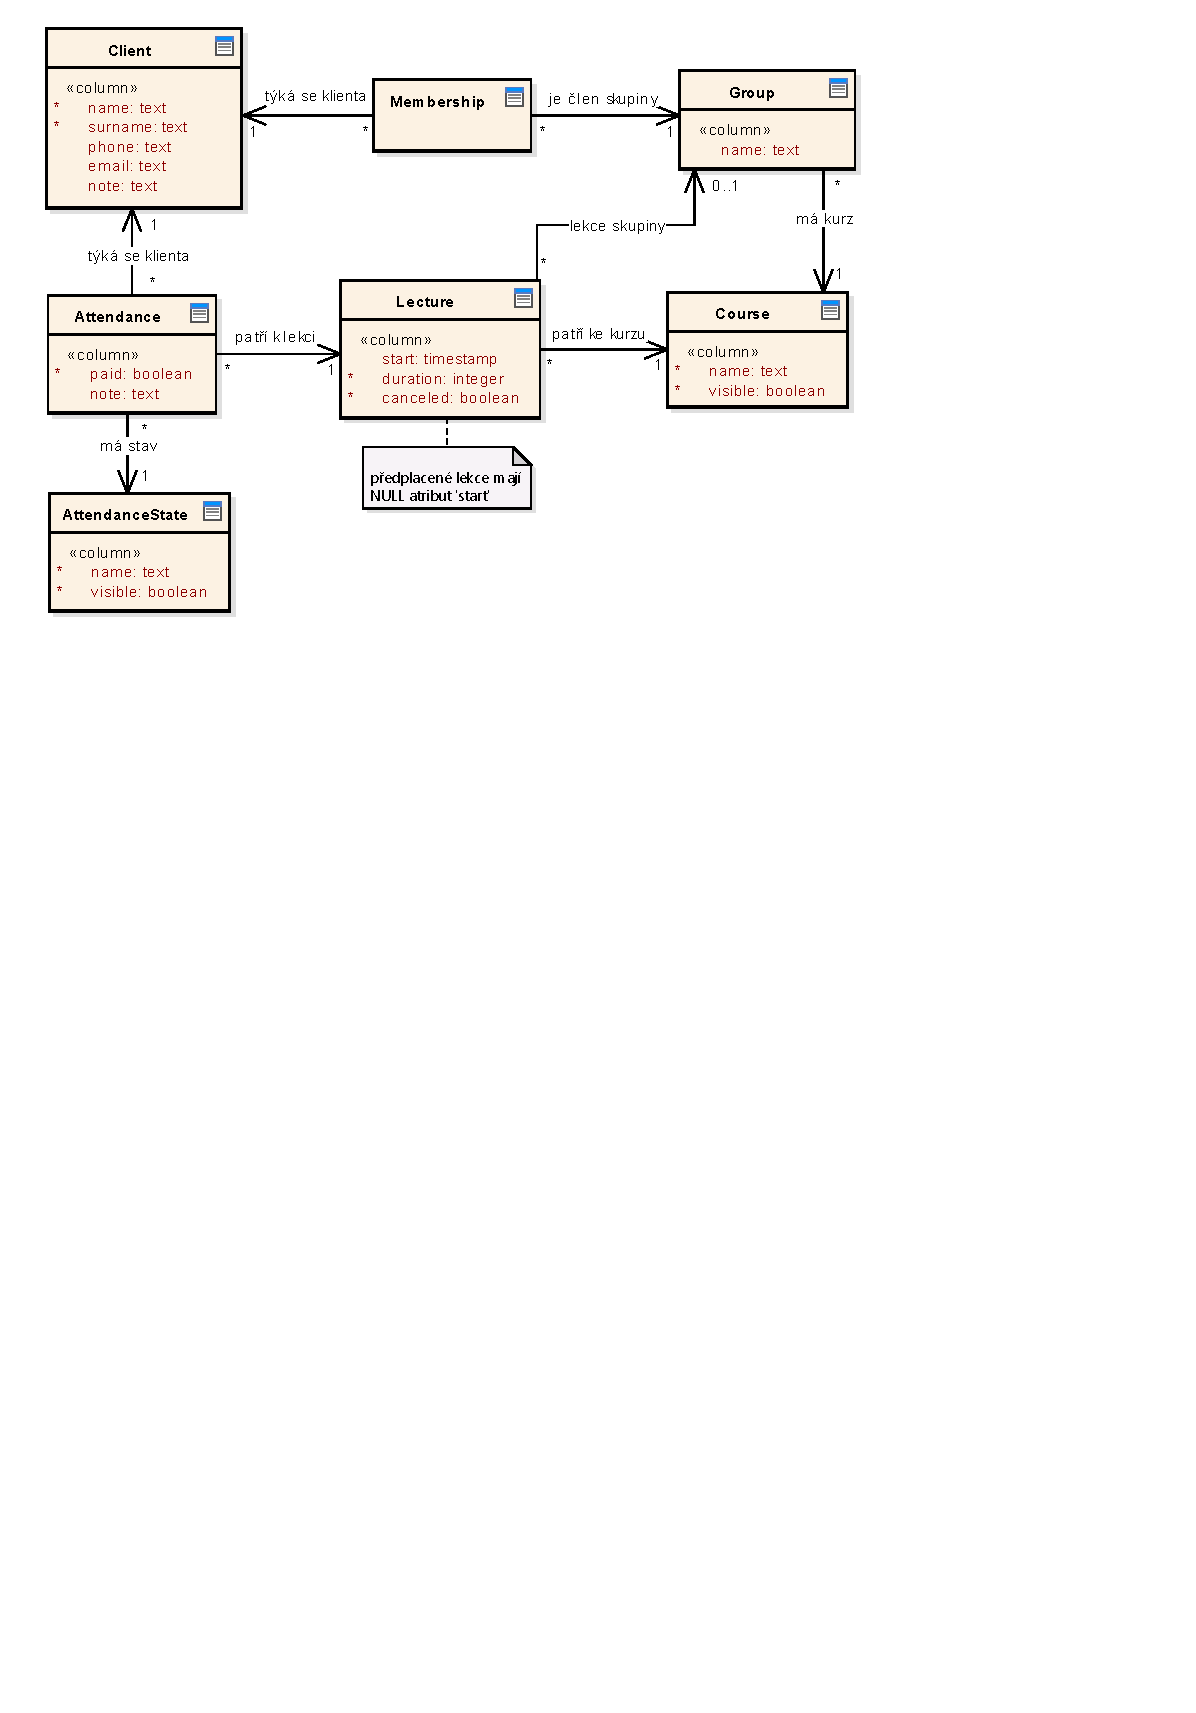
\includegraphics[width=1\textwidth]{img/db-model}
    	\caption[Logický datový model]{Logický datový model}\label{fig:db-model}
    \end{figure}
    
        \subsection{Client}
        Entita klienta slouží k evidenci informací o klientovi, vyžadováno je jméno a příjmení, nepovinně telefonní a e-mailový kontakt na rodiče a poznámka. Kontakty jsou nepovinně zejména kvůli tomu, že doteď nebyly evidovány na jednom místě a někdy dokonce vůbec a bude potřeba již stávající klienty do evidence samozřejmě přidat (viz. podsekce \ref{subsec:klienti}).
        
        \subsection{Membership}
        Členství slouží ke dvěma účelům. Zaprvé k dekompozici M:N vztahu klienta a skupiny (klient může být ve více skupinách a skupiny mohou mít více klientů), vím tedy, který klient patří do které skupiny. Zadruhé pro možné budoucí využití (původní záměr byl vytvořit atributy pro začátek a konec členství, na základě další analýzy a návrhů se ukázalo, že ale zatím postačí jednodušší varianta, tedy zda je teď členem nebo není).
        
        \subsection{Group}
        Entita skupiny slouží k evidenci jednotlivých skupin. Atribut jméno skupiny je nepovinný (ačkoliv bude obvykle používán, jeho použití není vyžadováno, protože to není nutné). Dále skupina ví, ke kterému kurzu náleží, tato vazba je zde proto, že skupiny už od počátku svého vytvoření patří vždy k právě jednomu kurzu (oproti klientovi, který takovou vazbu nepotřebuje).
        
        \subsection{Course}
        Kurzu drží dva atributy: jméno kurzu a viditelnost, oba jsou povinné. Viditelnost slouží k tomu, aby bylo v rámci aplikace možné při přidávání lekcí či skupiny skrýt z možností kurzu příslušný kurz, pokud už není provozován (aby byla zachována předchozí evidence lekcí daného kurzu).
        
        \subsection{AttendanceState}
        Stav účasti slouží k evidování možností stavu účasti klientů na kurzu, předpokládanými stavy jsou např. \enquote{omluven} a \enquote{nepřišel}. Tato entita drží dva atributy: název stavu účasti a viditelnost, oba jsou povinné. Viditelnost opět slouží k tomu, aby bylo v rámci aplikace možné pro nově přidávané lekce skrýt z možností stavu účasti klienta příslušný stav, pokud už není využívaný (aby byla zachována předchozí evidence lekcí daného kurzu). Tím, že mám jednu entitu, která říká, jaké jsou možné stavy účasti, může být aplikace konzistentní, zároveň pro úpravu názvu není potřeba upravit každý stav zvlášť, dále lze jednoduše stav účasti přidat a začít jej používat, případně jej přestat používat a skrýt z budoucích nabídek (nebo v případě žádného použití i smazat).
        
        \subsection{Attendance, Lecture}
        Vzhledem k úzkému propojení těchto dvou entit spojuji jejich popis do jedné podsekce. Účast a lekce jsou jádrem aplikace a vzhledem k tomu, že je k nim potřeba z různých entit přistupovat, bylo potřeba jim věnovat dostatečný čas v návrhu, aby byl kvalitní a nebylo nutné jej v průběhu vývoje měnit.
        
        Je potřeba evidovat lekce, každá má povinné atributy trvání (plánuje se funkcionalita upozornění na překryv lekcí), zda je zrušena (díky tomu lze jednoduše zrušit i skupinové lekce, oproti přístupu, kdy bychom zrušení evidovali prostřednictvím entity stavu účasti) a nepovinnou časovou značku začátku lekce (tzv. timestamp). V případě, že se jedná o naplánovanou lekci bez zatím známého konkrétního termínu, atribut začátku obsahuje hodnotu \verb|null|. Ke každé lekci eviduji k ní náležící právě jeden kurz a nepovinně také skupinu, pokud se nejedná o individuální kurz. Tato vazba je potřeba pro individuální lekce (skupiny jsou řešeny vazbou přímo z entity skupin), tento způsob byl shledán po vyhledávání alternativních možností tím nejvhodnějším.
        
        Entita účasti je úmyslně oddělena od lekce, aby každý klient, kterého se lekce týká, mohl mít své údaje o účasti (což je v případě skupiny potřeba). Každá účast tedy ví, ke které jedné lekci a jednomu klientovi náleží, a také je k ní navázán právě jeden stav účasti příslušného klienta.
        
        Příkladem budiž lekce z pohledu entity účasti -- pro případ individuální lekce má účast navázaného jednoho klienta, jeden stav účasti a jednu lekci, která je dále navázána na jeden kurz. Pro případ skupinové lekce se čtyřčlennou skupinou jsou využity 4 záznamy v klientech, jeden záznam ve skupině a tyto záznamy jsou spojeny entitou členství. Skupině náleží jeden kurz. Nyní mohu vytvořit pro každého z účastníků účast navázanou na každého z nich, na stav účasti a také všechny navázané na stejnou lekci.
        

    \section{Architektura}\label{architektura}
    Na obrázku \ref{fig:deployment-diagram} je diagram nasazení. Architektura má tři části: server, klient a databázový server. Na klientovi (počítač, telefon, tablet) běží webový prohlížeč. Na serveru běží webový server Gunicorn, což je Python WSGI HTTP Server (WSGI znamená, že splňuje požadavky na rozhraní Web Server Gate Interface, a tedy umožňuje komunikovat Django aplikaci, která WSGI vyžaduje, s webovým serverem). PostgreSQL databáze bude na samostatném serveru.
    
    \begin{figure}[ht]\centering
    	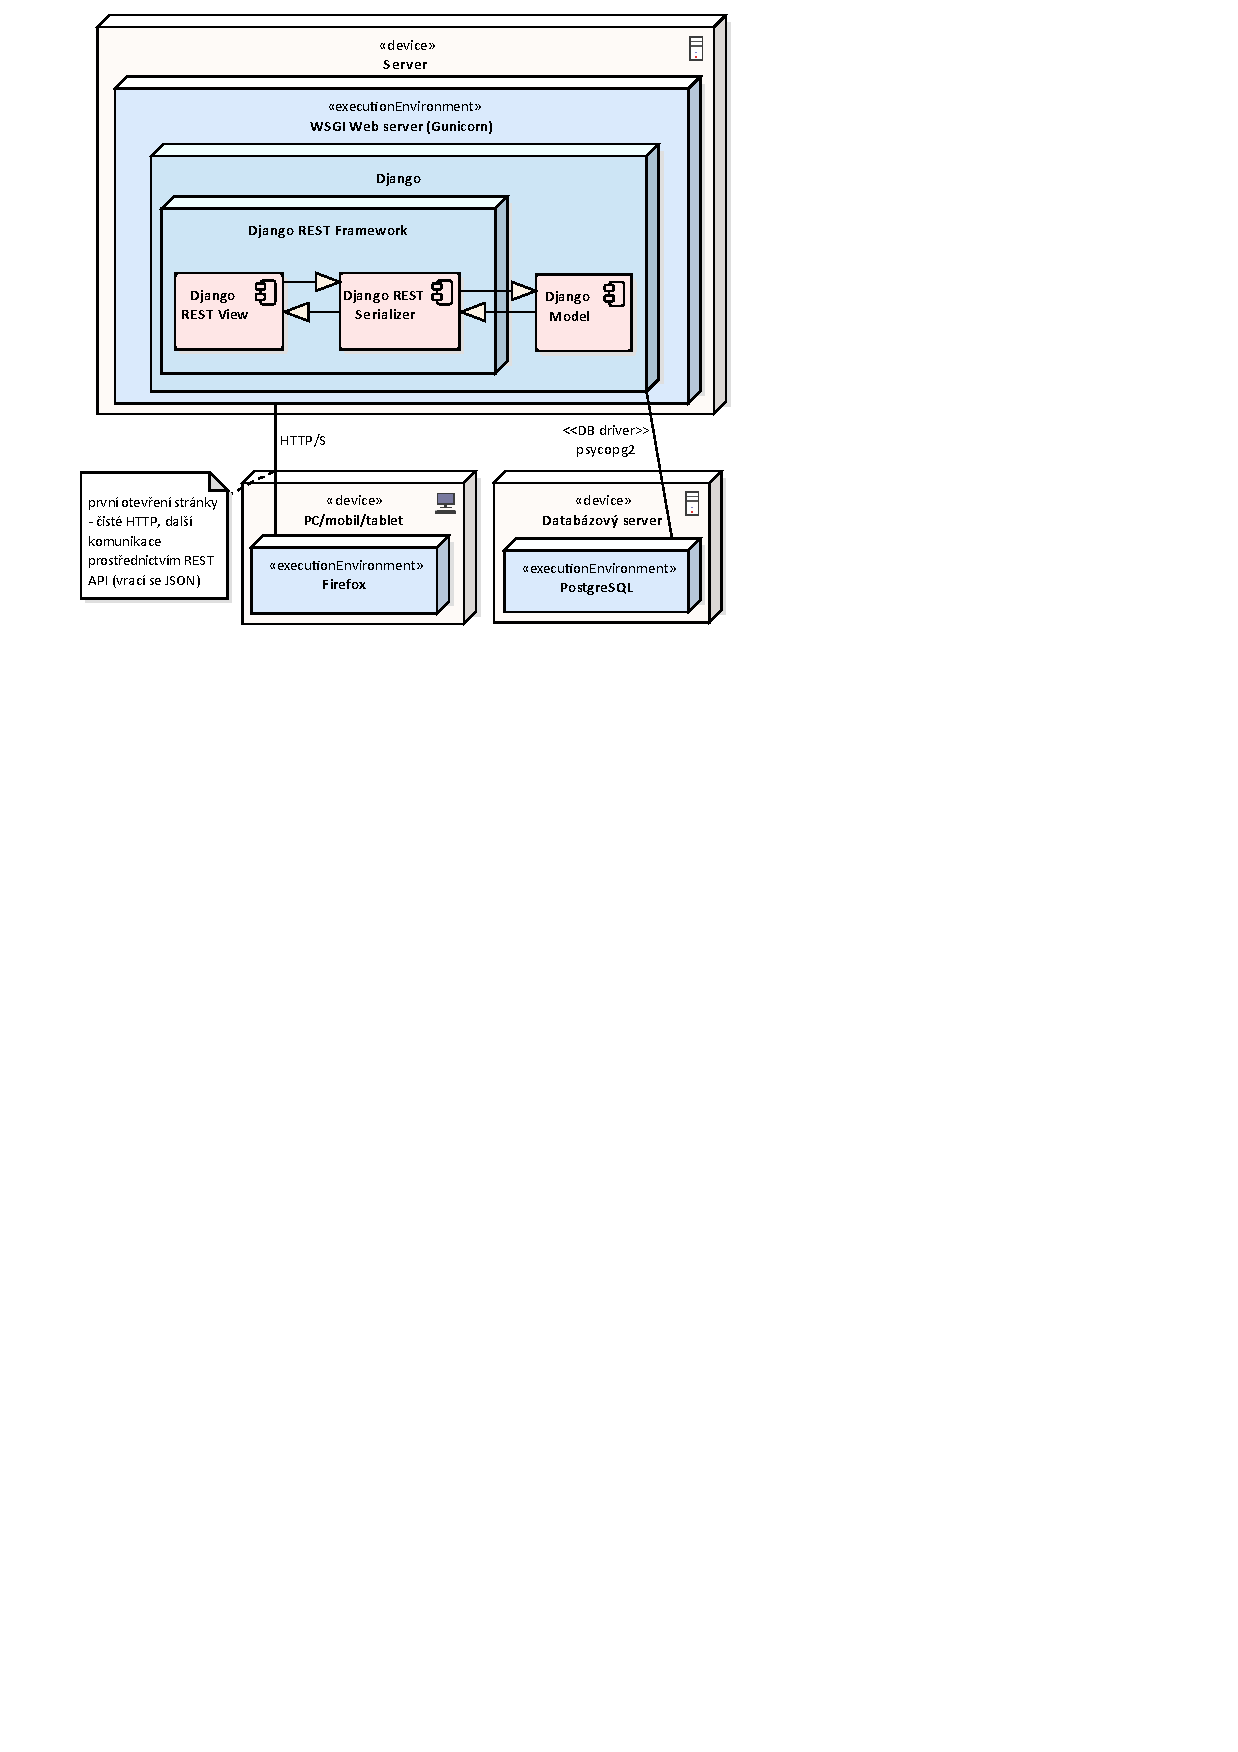
\includegraphics[width=1\textwidth]{img/deployment-diagram}
    	\caption[Diagram nasazení]{Diagram nasazení}\label{fig:deployment-diagram}
    \end{figure}
    
    Jak již bylo řečeno v sekci \ref{reseni}, serverová část je v jazyce Python a frameworku Django a s klientskou částí v jazyce Javascript a frameworku React komunikuje přes REST API ve formátu JSON. Django je postavené na architektuře MVT (popis v sekci \ref{mvc}) a React na architektuře CBA (popis v sekci \ref{cba}). První požadavek a odpověď budou čistě v HTTP/S, tedy klient požádá o stránku, server mu ji celou vrátí, další komunikace už bude probíhat přímo přes REST API a odpovědi budou v JSON (díky tomu může být aplikace SPA, viz. \ref{spampa}). Python, a tedy i Django, umí v základu komunikovat pouze s SQLite databází, pro další databáze je třeba využít adaptér -- pro PostgreSQL se používá psycopg2. O vyřízení API požadavků je požádán Django REST Framework, konkrétně část View, která poté prostřednictvím Serializeru využije příslušné Django Modely (tedy ORM) a z databáze tak získá data.
    
    \section{Uživatelské prostředí}
    Návrh uživatelského prostředí je neodmyslitelnou součástí tvorby webové aplikace. Vzhledem k tomu, že byl návrh tvořen v několika iteracích, zvolil jsem pohodlnější a rychlejší kreslení na papír. Díky tomu jsme při konverzaci nad budoucí podobou aplikace s lektorkou mohli některé nápady okamžitě zahodit a vytvořit bez problémů nové.
    
    \begin{figure}[ht]\centering
    	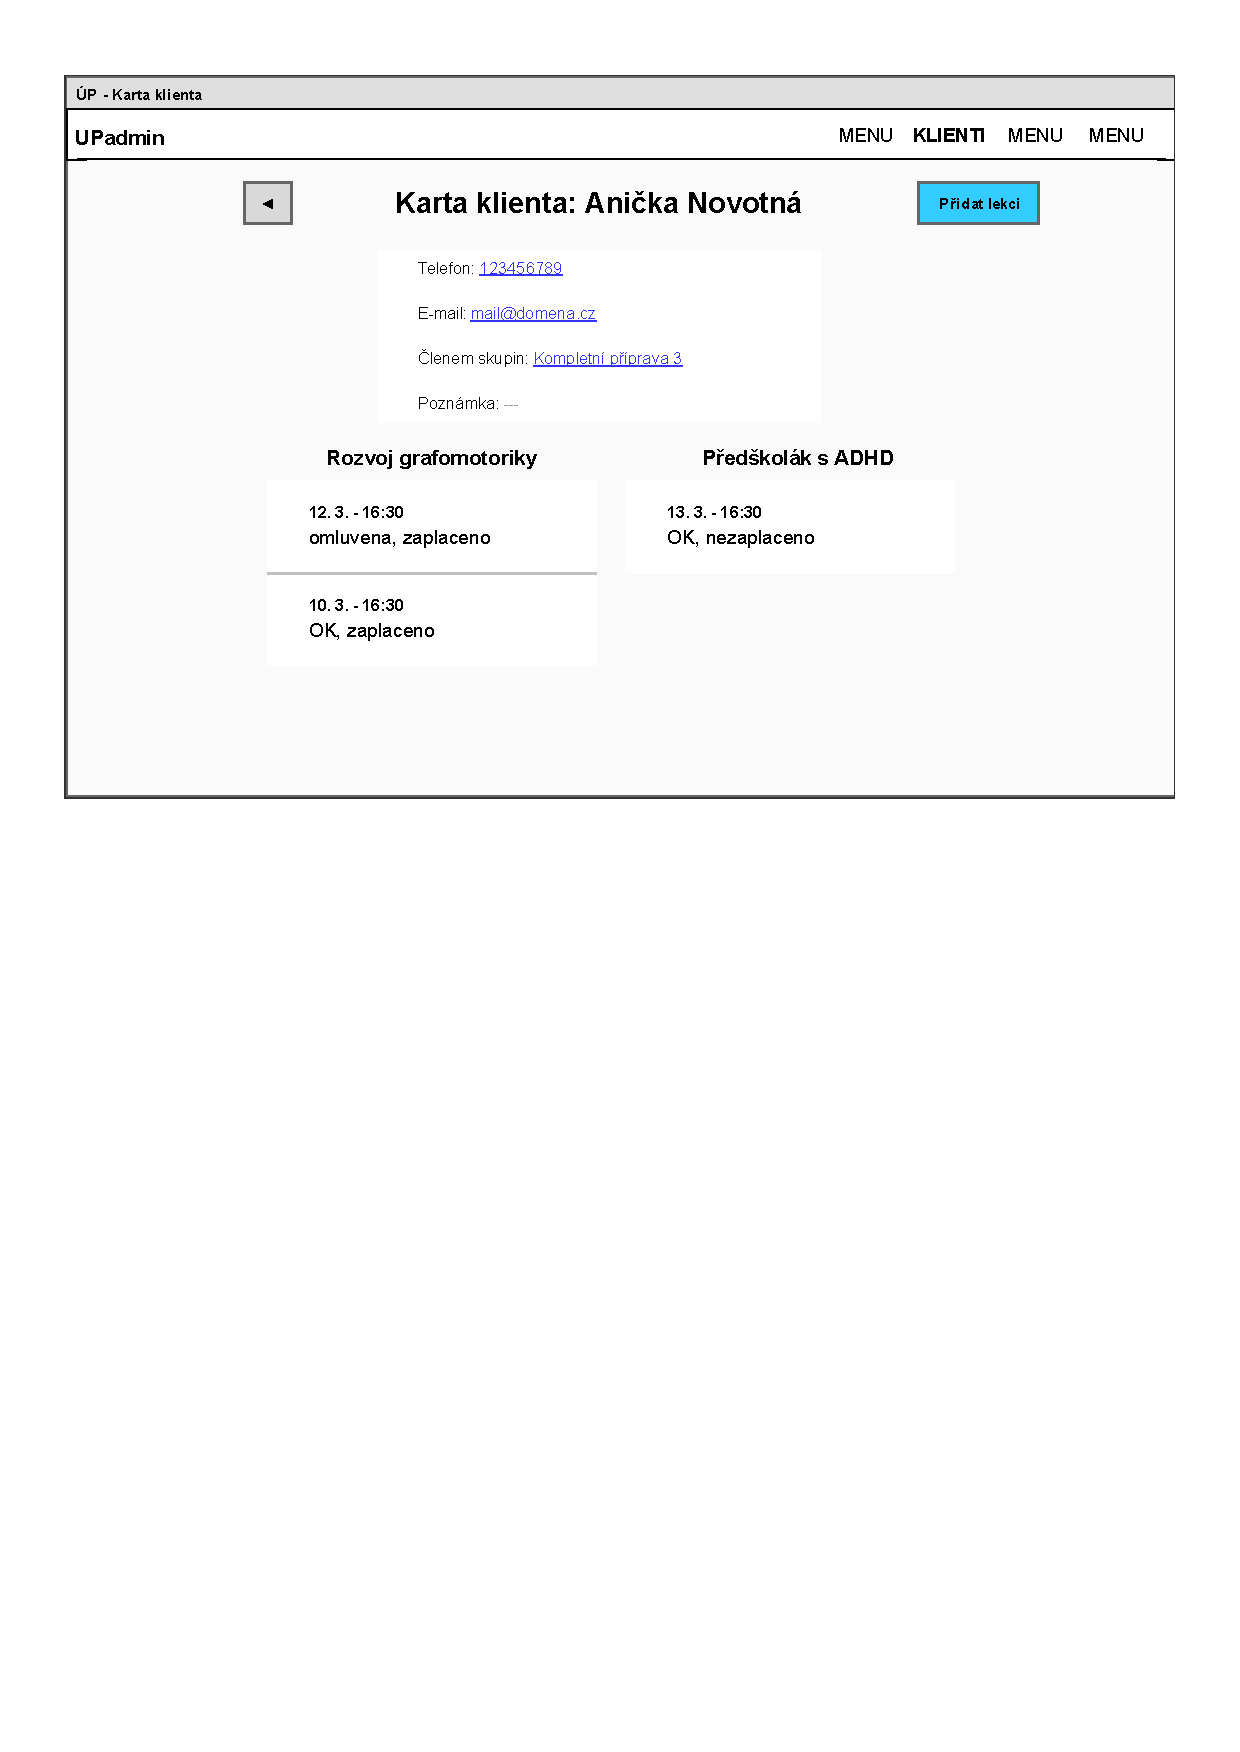
\includegraphics[width=1\textwidth]{img/ui-navrh}
    	\caption[Návrh karty klienta]{Návrh karty klienta}\label{fig:ui-navrh}
    \end{figure}
    
    Na obrázku \ref{fig:ui-navrh} je jeden z návrhů z poslední iterace překreslený z papíru do aplikace \href{https://pencil.evolus.vn/}{Pencil}, jedná se o návrh karty klienta. Na základě těchto návrhů jsme doiterovali až do stavu, kdy jsme přesně věděli, co od aplikace kde a jak čekat.
    
    \section{Komunikační rozhraní}
    Bylo potřeba navrhnout API tak, aby vystavilo všechny příslušné body potřebné pro práci na klientské části. Při návrhu jsem vycházel mj. z doporučení v \cite{api-bestpractises} -- pro všechny body jsou názvy v množném čísle, využívám naplno všechno dostupné HTTP metody GET, POST, PUT, PATCH a DELETE, nevystavuji zbytečně adresy obsahující prováděné akce (např. vytvoření) a adresa všech níže dále uvedených bodů API vždy začíná \verb|/api/v1/| (obsahuje tedy i označení verze API).
    
    Jak bylo již řečeno v předchozím odstavci, API kromě běžných operací umožňuje také PATCH požadavek, ten slouží k datově méně náročné částečné aktualizaci údajů. Tuto metodu lze použít například v případě označení lekce jako zaplacené -- v tomto případě není nutné přenášet další údaje, stačí \verb|id| a upravovaný údaj. GET požadavky často, z důvodu snížení počtu požadavků na server, rovnou obsahují zanořená data (která jsou stejně vždy potřeba).
    
    \newcommand{\apiA}{0.33}
    \newcommand{\apiB}{0.14}
    \newcommand{\apiC}{0.43}
    
        \subsection{Klienti}
        Bod pro klienty pracuje s klíči \verb|id|, \verb|name|, \verb|surname|, \verb|phone|, \verb|email| a \verb|note|.
        Pro GET požadavky jsou klienti seřazeni vždy podle abecedy vzestupně, a to podle příjmení a poté jména.
        
            {\centering
            \begin{tabular}{p{\apiA\textwidth}p{\apiB\textwidth}p{\apiC\textwidth}}&&\\
                \verb|clients/|             & \textbf{GET}      & vrátí všechny klienty\\
                \verb|clients/|             & \textbf{POST}     & vytvoření nového klienta\\
                \verb|clients/:id/|         & \textbf{GET}      & vrátí klienta s \verb|id|\\
                \verb|clients/:id/|         & \textbf{PUT}      & úprava klienta s \verb|id|\\
                \verb|clients/:id/|         & \textbf{PATCH}    & částečná úprava klienta s \verb|id|\\
                \verb|clients/:id/|         & \textbf{DELETE}   & smazání klienta s \verb|id| (lze smazat pouze pokud nemá žádné lekce)\\
            \end{tabular}}
            
        \subsection{Lekce}
        Bod pro lekce pracuje s klíči \verb|id|, \verb|start|, \verb|group|, \verb|canceled| a \verb|duration|, to ale není vše. V případě skupinové lekce klíč \verb|group| obsahuje zanořené informace o skupině. Součástí odpovědi jsou i zanořené informace o kurzu (klíč \verb|course|) a jednotlivých účastech klientů (klíč \verb|attendances|), které obsahují platbu (klíč \verb|paid|), poznámku (klíč \verb|note|) a navíc také zanořené informace o každém z klientů (klíč \verb|client|), stavu účasti (klíč \verb|attendancestate|), vypočítané informace o číslu lekce v pořadí (klíč \verb|count|) a zda je potřeba připomenout příští platbu (klíč \verb|remind_pay|). Vypočítané informace jsou pouze v odpovědích a při požadavcích na úpravu či vytvoření se neuvádějí, dále zanořené informace kromě samotných účastí se zadávají pouze formou \verb|klíč_id| (tedy např. \verb|attendancestate_id|).
        
        Každý z dotazů na lekce lze doplnit také o parametr \verb|ordering=start|, resp. \verb|ordering=-start| pro seřazení výsledků dle atributu \verb|start| vzestupně, resp. sestupně (s posledními třemi dotazy, které již výsledky filtrují, lze toto řazení připojit přes operátor \verb|&|), výchozí řazení je sestupně (tedy od posledních lekcí k nejstarším). Kromě dotazu s uvedeným přesným datumem v parametru se vrací i zrušené lekce.
        
            {\centering
            \begin{tabular}{p{\apiA\textwidth} p{\apiB\textwidth} p{\apiC\textwidth}}&&\\
                \verb|lectures/|            & \textbf{GET}      & vrátí všechny lekce\\
                \verb|lectures/|            & \textbf{POST}     & vytvoří novou lekci\\
                \verb|lectures/:id/|        & \textbf{GET}      & vrátí lekci s \verb|id|\\
                \verb|lectures/:id/|        & \textbf{PUT}      & úprava lekce s \verb|id|\\
                \verb|lectures/:id/|        & \textbf{PATCH}    & částečná úprava lekce s \verb|id|\\
                \verb|lectures/:id/|        & \textbf{DELETE}   & smazání lekce s \verb|id|\\
                \verb|lectures/?group=:id|  & \textbf{GET}      & vrátí lekce skupiny s \verb|id|\\
                \verb|lectures/?client=:id| & \textbf{GET}      & vrátí lekce klienta s \verb|id| (jen individuální)\\
                \verb|lectures/?date=:date| & \textbf{GET}      & vrátí lekce (bez zrušených) konající se v zadaný datum \verb|date| (ve formátu YYYY-mm-dd)\\ %ISO
            \end{tabular}}
        
        \subsection{Skupiny}
        Bod pro lekce pracuje s klíči \verb|id|, \verb|name| a dále se zanořenými informacemi o kurzu (klíč \verb|course|) a  členech skupiny (klíč \verb|memberships|) se zanořenými informacemi o klientovi (klíč \verb|client|). Pro úpravy a vytváření se opět místo zanoření atributy zadávají pouze formou \verb|klíč_id|.
        
            {\centering
            \begin{tabular}{p{\apiA\textwidth} p{\apiB\textwidth} p{\apiC\textwidth}}&&\\
                \verb|groups/|              & \textbf{GET}      & vrátí všechny skupiny\\
                \verb|groups/|              & \textbf{POST}     & vytvoří novou skupinu\\
                \verb|groups/:id/|          & \textbf{GET}      & vrátí skupinu s \verb|id|\\
                \verb|groups/:id/|          & \textbf{PUT}      & úprava skupiny s \verb|id|\\
                \verb|groups/:id/|          & \textbf{PATCH}    & částečná úprava skupiny s \verb|id|\\
                \verb|groups/:id/|          & \textbf{DELETE}   & smazání skupiny s \verb|id|\\
                \verb|groups/?client=:id|   & \textbf{GET}      & vrátí skupiny klienta s \verb|id|\\
            \end{tabular}}
        
        \subsection{Kurzy}
        Bod pro kurzy pracuje s klíči \verb|id|, \verb|name| a \verb|visible|.
        
            {\centering
            \begin{tabular}{p{\apiA\textwidth} p{\apiB\textwidth} p{\apiC\textwidth}}&&\\
                \verb|courses/|             & \textbf{GET}      & vrátí všechny kurzy\\
                \verb|courses/|             & \textbf{POST}     & vytvoří nový kurz\\
                \verb|courses/:id/|         & \textbf{GET}      & vrátí kurz s \verb|id|\\
                \verb|courses/:id/|         & \textbf{PUT}      & úprava kurzu s \verb|id|\\
                \verb|courses/:id/|         & \textbf{PATCH}    & částečná úprava kurzu s \verb|id|\\
                \verb|courses/:id/|         & \textbf{DELETE}   & smazání kurzu s \verb|id| (lze smazat pouze pokud není přiřazený k žádné lekci nebo skupině)\\
            \end{tabular}}
            
        \subsection{Stavy účasti}
        Bod pro stavy účasti pracuje s klíči \verb|id|, \verb|name| a \verb|visible|.
        
            {\centering
            \begin{tabular}{p{\apiA\textwidth} p{\apiB\textwidth} p{\apiC\textwidth}}&&\\
                \verb|attendancestates/|    & \textbf{GET}      & vrátí všechny stavy účasti\\
                \verb|attendancestates/|    & \textbf{POST}     & vytvoří nový stav účasti\\
                \verb|attendancestates/:id/|& \textbf{GET}      & vrátí stav účasti s \verb|id|\\
                \verb|attendancestates/:id/|& \textbf{PUT}      & úprava stavu účasti s \verb|id|\\
                \verb|attendancestates/:id/|& \textbf{PATCH}    & částečná úprava stavu účasti s \verb|id|\\
                \verb|attendancestates/:id/|& \textbf{DELETE}   & smazání stavu účasti s \verb|id| (lze smazat pouze pokud není přiřazený k žádné účasti)\\
            \end{tabular}}
            
        \subsection{Účasti}
        Bod pro účasti je vytvořen pro snížení datové náročnosti běžné prováděných úprav. Pracuje s klíči \verb|id|, \verb|paid|, \verb|note|, \verb|attendancestate_id| a \verb|client_id|.
        
            {\centering
            \begin{tabular}{p{\apiA\textwidth} p{\apiB\textwidth} p{\apiC\textwidth}}&&\\
                \verb|attendances/:id/|     & \textbf{PUT}      & úprava účasti s \verb|id|\\
                \verb|attendances/:id/|     & \textbf{PATCH}    & částečná úprava účasti s \verb|id|\\
            \end{tabular}}
            
        \subsection{Přihlášení}
        Bod pro účasti pracuje s klíči \verb|username|, \verb|password| a \verb|token|.
        
            {\centering
            \begin{tabular}{p{\apiA\textwidth} p{\apiB\textwidth} p{\apiC\textwidth}}&&\\
                \verb|jwt-auth/|            & \textbf{POST}     & na základě zaslaných údajů uživatele vrátí token\\
                \verb|jwt-refresh/|         & \textbf{POST}     & na základě zaslaného (neexpirovaného) tokenu vrátí nový obnovený token\\
            \end{tabular}}
            
    
\chapter{Implementace}
V této kapitole představím průběh samotné implementace. Je rozdělena do několika částí, nejprve popíši nástroje použité pro vývoj a přípravu prostředí, poté se zaměřím na vytvoření základního nastavení serverové a klientské části, které bude výchozím krokem pro další sekce, ve kterých postupně ukážu práci s datovou částí a tvorbu API. Tím připravím všechny součásti potřebné k fungování a vytvoření plnohodnotné klientské části v další sekci, uvedu zde také způsob komunikace se serverovou částí, tvorbu UI a další způsoby práce s JS a Reactem. Na závěr uvedu způsoby řešení bezpečnosti v aplikaci.

Nejproblematičtější fází se překvapivě stala konfigurace Djanga a Reactu tak, aby spolu tyto dvě části fungovaly, a také pokročilejší přizpůsobení API. Oběma problémům se budu také v této kapitole věnovat.

    \section{Nástroje pro vývoj}\label{nastrojeprovyvoj}
    Celá práce byla implementována ve vývojovém prostředí \href{https://www.jetbrains.com/pycharm/}{Pycharm Professional Edition} od Jetbrains na systému Windows 10, které nabízí nativní podporu pro všechny části tohoto projektu od samotného Pythonu (např. už ve výchozím nastavení podporuje virtuální prostředí pro izolaci jednotlivých prostředí pro různé projekty), Djanga až po React. Díky tomu lze využít všechny funkce tohoto vývojového prostředí pro všechny používané jazyky a frameworky a také lze většina úkonů provádět také pomocí grafického prostředí -- integrovaný terminál lze použít jen v případě, kdy je to opravdu potřeba. Dále existuje mnoho doplňků, které funkci IDE rozšíří o podporu dalších funkcí, např. pro lepší práci s verzovacími nástroji a YAML formátem.
    
    Pro rychlejší vývoj, organizaci a také pro rozšíření znalostí a zkušeností jsem se rozhodl využít i další služby. Pro verzování využívám soukromý repozitář na \href{https://github.com/}{GitHubu}. Dále používám nástroj pro průběžnou integraci a dodávání \href{https://travis-ci.com/}{Travis CI}. Díky jednoduchému propojení s GitHubem se tak mohou samy spouštět při každém nahrání nové verze testy včetně těch pokročilejších a náročnějších a v případě úspěchu se aplikace nahraje na produkční server pro zákazníka. K tomu všemu slouží jediný soubor v kořenovém adresáři s názvem \verb|.travis.yml|, podrobněji příslušné části souboru popíši v kapitolách o testování \ref{testovani} a nasazení \ref{nasazeni}.
    
    \section{Příprava prostředí}
    Pro vývoj je potřeba nainstalovat další potřebné balíčky a závislosti, nejdříve jsem tedy nainstaloval do systému Python, jehož součástí je balíčkovací systém pip pro instalaci knihoven, a Node.js, jehož součástí je balíčkovací systém pro JS s názvem npm (Node.js je potřeba především pro vývoj, vytváření buildů a běh vývojového serveru, npm je vítaným ulehčením práce s knihovnami a závislostmi). V současnosti se často používá také balíčkovací systém yarn, který je ale třeba doinstalovat (například přes npm), jeho výhodou jsou stejné principy jako npm, ale mnohem vyšší efektivita a rychlost \cite{yarn}, pro tento projekt jej tedy z těchto důvodů používám. Pomocí těchto balíčkovacích systémů jsem dále nainstaloval poslední verze frameworku \href{https://www.djangoproject.com/}{Django} a nástroj \href{https://github.com/facebook/create-react-app}{create-react-app} pro jednoduché vytvoření React aplikace. Vzhledem k tomu, že vývoj bude probíhat v Pycharmu, není již potřeba dále řešit virtuální prostředí v Pythonu. Na závěr samozřejmě přidám a připravím v systému databázi PostgreSQL.
    
    \section{Základní nastavení serverové a klientské části}\label{zakladninastaveni}
    Začnu nejprve serverovou částí. V Djangu je potřeba nejprve vytvořit projekt a do něj poté přidávat jednotlivé komponenty, kterým se říká aplikace, projekt je tedy soubor aplikací a nastavení na jedné doméně. Pro vytvoření základní kostry projektu s výchozím nastavením jsem využil možností rozhraní Pycharmu, díky kterému stačí vyplnit základní informace o aplikaci a celou kostru připraví za mě, vytvořil jsem tedy projekt \verb|up|. Pro vytvoření aplikací jsem využil vestavěného manage.py terminálu v Pycharmu a v něm jsem přes příkaz \verb|startapp| vytvořil dvě aplikace: \verb|admin| (pro samotnou aplikaci) a \verb|api| (pro API). Ty je poté potřeba v nastavení Djanga přidat do seznamu \verb|INSTALLED_APPS| v souboru s nastavením.
    
    \begin{listing}[ht]
    	\begin{minted}{python}
re_path(r'^', TemplateView.as_view(template_name="index.html"))
    	\end{minted}
    	\caption{Základní nastavení routování v urls.py}\label{lst:urls.py}
    \end{listing}
    
    Do serverové části zatím nebudu v této sekci příliš zasahovat, pro další práci ještě ale upravím aplikaci \verb|admin| tak, aby místo své výchozí stránky zobrazovala mou vlastní. Pro takto jednoduché zobrazení stačí využít již připravený generický pohled \verb|TemplateView| a jeho metodu \verb|as_view|, tedy do souboru \verb|urls.py| vložím kód \ref{lst:urls.py}, který zařídí, že každému uživateli na jakékoliv adrese (kromě API, to nastavím až v sekci \ref{sec:api}) ukážu daný soubor (zobrazit klientovi správnou stránku v rámci webové aplikace bude zodpovědnost JS na klientské části).
    
    Serverová část je připravena, nyní popíši základní nastavení klientské části. Nástroj create-react-app umožňuje jednoduše vytvořit základní React aplikaci včetně všech základních nastavení a kostry. Takto jsem vytvořil aplikaci \enquote{frontend}, tedy složku s tímto názvem, která obsahuje všechny potřebné součásti pro běh React aplikace. Součástí této připravené aplikace jsou mimo jiné tyto předkonfigurované součásti:
    \begin{itemize}
        \item transpiler Babel, který umožní používat bez obav JSX a další nové funkce z novějších ES standardů (viz. sekce \ref{js}),
        \item bundlovací nástroj Webpack, který umožňuje \cite{webpack-ackee}:
            \begin{itemize}
                \item rozdělovat kód do modulů a napříč aplikací je importovat a znovupoužívat,
                \item spouštět server, který umožní rychlý vývoj díky \enquote{hot reloadingu} (tedy okamžité automatické projevení změn při úpravě kódu),
                \item automaticky spouštět transpilaci Babelem,
                \item po přeložení vytvořit ze všech modulů a částí kódu jeden či více balíčků, které pak lze jako běžné JS a další soubory (např. CSS) servírovat na produkci, kde už vývojový server neběží,
                \item s produkčními soubory provést obfuskace (minifikaci, uglifikaci), komprimaci, označení hashem (aby prohlížeč poznal, zda může využít soubor z cache, nebo došlo ke změnám) -- ,
            \end{itemize}
        \item testovací nástroje a další knihovny umožňující rychlejší vývoj, vyšší kompatibilitu napříč prohlížeči, rychlejší načítání ad.
    \end{itemize}
    Všechny tyto součásti používám, včetně nových specifikací ECMAScript, JSX apod., díky všem nástrojům není důvod k obávám z nekompatibility a můžu z jejich použití pouze profitovat. Uvedené operace se soubory, které provádí Webpack a Babel by většinou šly provést až na produkci u uživatele, ale jednalo by se o zbytečně krkolomné a pomalé řešení, proto se provádí již při nahrávání na testovací/produkční server.
    
    Nyní tedy mám na lokálním počítači připravené Django, které mi díky svému vývojovému serveru zobrazí výchozí stránku a React, který mi díky Webpack vývojovému serveru zobrazí na odlišném portu také svou výchozí stránku. Je třeba tyto dvě části propojit. V případě lokálního prostředí musí spolupracovat tak, abych nepřišel o žádné výhody jako např. hot reloading, hash v názvu, tedy aby nebylo při každé úpravě potřeba v Djangu měnit adresu souborů kvůli odlišné hodnotě hashe). V případě produkčního prostředí je třeba přizpůsobit konfiguraci tomu, že zde už poběží pouze jeden server (Gunicorn), na kterém bude běžet Django. Tato část se vzhledem k mé dosavadní neznalosti těchto technologií ukázala jako poměrně náročná, protože bylo potřeba upravit kódy na obou stranách (tedy jak v Djangu, tak pro React v konfiguraci Webpacku) a ještě k tomu toto udělat prakticky dvakrát, jak pro lokální vývoj, tak pak odlišně pro produkci. Nakonec se mi ale podařilo tuto problematiku vyřešit, řešení vychází z článku \cite{webpack-loader2} a také staršího článku autora obou použitých knihoven \cite{webpack-loader1}, v následujícím odstavci jej stručně popíši.
    
    Díky nástroji create-react-app \cite{cra} mám k dispozici jednoduchou kostru, která mi ale neumožní hlubší zásahy do další konfigurace vnitřních součástí. Je tedy potřeba pomocí příkazu \verb|yarn eject| \enquote{vysunout} konfigurační soubory a závislosti tak, abych k nim měl přístup a mohl je upravit. Nyní potřebuji dvě další dvě knihovny, každou pro jednu stranu -- do JS přidám knihovnu \href{https://github.com/owais/webpack-bundle-tracker}{webpack-bundle-tracker} (dále jen tracker), která vyextrahuje potřebné informace z Webpacku do JSONu \cite{webpack-bundle-tracker} (např. názvy vygenerovaných souborů) a do Djanga přidám knihovnu \href{https://github.com/owais/django-webpack-loader}{django-webpack-loader} (dále jen loader), která tyto informace bude konzumovat a umožní použít vygenerované soubory Webpackem v Djangu \cite{django-webpack-loader}. Tento JSON soubor bude tedy propojovat Webpack s Djangem.
    
    Když mám připravené tyto knihovny a kompletní kostru aplikace po vysunutí, je potřeba upravit konfiguraci Webpacku pro lokální i produkční prostředí tak, aby spolupracoval s trackerem a soubory byly tam, kde je bude očekávat loader, který bude konzumovat výstup trackeru (a aby totéž umožnil i pro lokální prostředí s hot reloadingem). Také je potřeba nakonfigurovat loader, to lze provést v souboru s nastavením Djanga, oproti původní vygenerované kostře Djangem budou ale soubory s nastavením dva, jeden obecný, jehož součástí budou také informace pro lokální prostředí a jeden produkční, který bude obsahovat import předchozího a přetíží konfiguraci potřebných částí tou svojí (to se týká nejen této části, ale později například i různých nastavení databází pro různá prostředí). V těchto nastaveních jsem nakonfiguroval loader tak, aby konzumoval správný soubor ze správného místa a také jsem nastavil adresy statických souborů tak, aby je Django zahrnulo do shromažďování souborů prováděného příkazem \verb|collectstatic| (používá se při nasazení). Posledním krokem je vložení Djangem získaných souborů do webové stránky, aby se zobrazily uživateli, v tomto kroku tedy poprvé a naposledy v celé této práci použiji šablonovací systém Djanga (který by byl naopak hojně používaný v případě, že bych nezvolil architekturu) -- do kostry výchozí stránky Djanga vložím tagy, které z loaderu umístí příslušné soubory do stránky (tedy JS a CSS). Je hotovo, po provedení příkazu \verb|manage.py runserver| a \verb|yarn start| Django ukazuje webovou stránku, na které je zobrazena výchozí stránka Reactu, a to jak v lokálním prostředí, tak na produkci. Výchozí zjednodušená stránka, která zaručí zobrazení celé aplikace je na ukázce \ref{lst:html}. React aplikace se vkládá do elementu \verb|root|.
    
    \begin{listing}[ht]
    	\begin{minted}{html}

<!DOCTYPE html>
<html lang="cs">
<head>
    <meta charset="UTF-8"/>
    <meta name="viewport" content="width=device-width,
                                   initial-scale=1,
                                   shrink-to-fit=no">
    <title>ÚPadmin</title>
</head>
<body>
<div id="root">
    <h2>Načítání...</h2>
</div>

</body>
</html>
    	\end{minted}
    	\caption{Základní stránka webové aplikace}\label{lst:html}
    \end{listing}
    
    \section{Datová část}\label{sec:datovaCast}
    K již nainstalovanému PostgreSQL jsem ještě nainstaloval vývojové prostředí pro databáze od Jetbrains s názvem DataGrip, díky kterému budu moci jednoduše nahlížet jak do lokální databáze, tak do databáze na produkčním serveru a případně provádět i další operace. Jak jsem již zmínil v sekci s návrhem architektury \ref{architektura}, je potřeba použít adaptér \href{http://initd.org/psycopg/}{psycopg2}, ten umožní v Pythonu, a tedy i Djangu, používat databázi PostgreSQL. Do nastavení Djanga přidám tuto databázi a zbývá definovat tabulky v databázi.
    
    Při návrhu datového modelu v sekci \ref{datovymodel} jsem nastínil, že díky frameworku mám výrazně ulehčenou práci s databází (a je třeba říci, že pokud člověk doteď žádný framework s touto funkcionalitou nepoužíval, je to opravdu obrovský krok kupředu), v Djangu není potřeba mít skripty pro vytvoření databáze, jediným zdrojem pravdy jsou Django modely definující jednotlivé entity, jejich atributy a chování. Následné další úpravy databáze na základě modelů se provádí prostřednictvím takzvaných migrací. V ukázce \ref{lst:models} je jeden z modelů, konkrétně lekce, vybral jsem jej proto, že je na něm možné ukázat více věcí -- je zde vidět pět atributů, některé jsou nepovinné (\verb|start| a \verb|group|), reprezentují různé typy polí (kladné číslo, cizí klíč, boolean, časová značka) a u cizích klíčů je vidět, na který model odkazují, mohou mít přidělené jméno (použije se při využití opačného vztahu v modelu skupin) a také mají definované chování při smazání příslušného záznamu, tedy kurz se podaří smazat pouze když k němu nejsou žádné lekce (ošetření, aby se omylem nepřišlo o záznamy z historie) a v případě smazání skupiny se smažou mj. všechny její lekce.
    
    \begin{listing}[ht]
    	\begin{minted}{python}
class Lecture(models.Model):
    start = models.DateTimeField(null=True)
    canceled = models.BooleanField()
    duration = models.PositiveIntegerField()
    course = models.ForeignKey(Course, on_delete=models.PROTECT)
    group = models.ForeignKey(Group, related_name='lectures',
                              on_delete=models.CASCADE,
                              null=True)
    	\end{minted}
    	\caption{Ukázka modelu lekce ze souboru models.py}\label{lst:models}
    \end{listing}
    
    Postup při používání zmíněných migrací je jednoduchý. Při vytvoření či úpravě modelů je potřeba zavolat \verb|manage.py makemigrations| (vytvoří soubor s migracemi na základě provedených úprav, v případě nejasností nebo potřebě dalších informací mě vyzve k doplnění, tedy např. pokud měním atribut z nepovinného na povinný, vyzve mě k zadání výchozí hodnoty, která bude doplněna do stávajících záznamů bez vyplněného atributu) a poté změny aplikovat \verb|manage.py migrate|. V praxi tedy při vývoji upravím model, vytvořím příslušným příkazem soubor s migracemi (a s tím související doplňující informace), zkontroluji správné výsledky a funkčnost a výsledek zašlu do verzovacího systému, Travis a Heroku poté provedou příslušné migrace a změny jsou úspěšně provedeny ve všech prostředích konzistentně. Také je třeba dodat, že první migrací nevzniknou pouze mnou definované tabulky, ale také pomocné tabulky Djanga potřebné pro správný chod (např. tabulka s uživateli, provedenými migracemi ad.).
    
    \section{API}\label{sec:api}
    Mám připravený základ serverové části, tedy Djanga, které servíruje stránku s React aplikací a také modely Djanga, které umožní pracovat s entitami v projektu. Je potřeba vytvořit REST API, které umožní Reactu komunikovat se serverovou částí. V této části stručně shrnu, jak tvorba API probíhala. Vzhledem k tomu, že s tvorbou API je spojeno spoustu opakování podobného kódu, rozhodl jsem se využít služby dalšího frameworku, který mi v Djangu obstará jednoduché vytvoření REST API. Frameworků existuje několik, zvolil jsem nejpopulárnější, \href{http://www.django-rest-framework.org/}{Django REST Framework} (dále DRF), který poskytuje užitečné nástroje a konstrukty k efektivní tvorbě API a zároveň obsahuje velkou škálu doplňkových knihoven od dalších členů komunity, které lze také využít \cite{drf2}. Pro následné testování a úpravy API jsem používal nástroj \href{https://www.getpostman.com/}{Postman}.
    
    Obecně se tvorba API v DRF dělí na několik částí: views (pohledy), serializery a URL mapování. Nejprve je potřeba zvolit URL adresu pro API požadavky, tato adresa bude jako jediná mít zvláštní chování, ostatní adresy jsou obslouženy Reactem (viz. nastavení v sekci \ref{zakladninastaveni}). Před řádek v ukázce kódu \ref{lst:urls.py} vložím další řádek uvedený v ukázce \ref{lst:urls.py2} (pokud bych jej vložil za, tak vzhledem k působnosti dříve vloženého kódu by převzal zodpovědnost za API React, což nechci). Nyní už stačí definovat konečné URL body API, kde určím, která adresa využije který pohled, k tomu slouží v DRF router, který umožní v souboru \verb|api/urls.py| jednoduchým způsobem definovat spojení URL adres s pohledy, v ukázce kódu \ref{lst:apirouter} uvádím část pro lepší pochopení -- vybral jsem dva pohledy, které v dalším odstavci podrobněji ve zkratce představím a ukážu na nich další kroky při tvorbě API.
    
    \begin{listing}[ht]
    	\begin{minted}{python}
path('api/v1/', include('api.urls')),
    	\end{minted}
    	\caption{Nastavení routování pro API v souboru urls.py}\label{lst:urls.py2}
    \end{listing}
    
    \begin{listing}[ht]
    	\begin{minted}{python}
router = routers.DefaultRouter()
router.register('courses', views.CourseViewSet)
router.register('groups', views.GroupViewSet)
    	\end{minted}
    	\caption{Ukázka routeru pro API v souboru api/urls.py}\label{lst:apirouter}
    \end{listing}
    
    DRF nabízí několik možností, jak vyřešit pohledy. Zvolil jsem tu, která by měla umožnit velmi jednoduše definovat celé API a obstarat automaticky pohled jak na detail (instanci entity), tak na kolekci (všechny instance entity) včetně všech operací, nazývá se ViewSet a API pohledy úzce mapuje na Django modely. Pohled může být definován poměrně snadno, jak je vidět v ukázce kódu \ref{lst:apiview1} ze souboru \verb|api/views.py| -- vytvořil jsem pohled pro kurzy, definoval jsem \verb|queryset|, tedy dotaz, který získá obsah pro odpověď na požadavek na API (v tomto případě i seřazený podle jména, to je definováno v modelu) a \verb|serializer_class|, tedy třídu použitou pro serializaci, validaci a deserializaci dat. Serializeru se budu věnovat v dalším odstavci. V druhé ukázce kódu pohledu \ref{lst:apiview2} je vidět, že přetěžuji metodu \verb|get_queryset|, to mi umožní vrátit v API odpovědi vyfiltrované výsledky, v tomto případě vrátím buď všechny skupiny (seřazené podle jména, to je definováno v modelu), nebo v případě zadání \verb|id| klienta všechny skupiny (opět seřazené podle jména), ve kterých je členem. Pro pokročilejší filtrování v API a také umožnění řazení přes parametry v adrese je pak u některých dalších pohledů využita knihovna django-filter, díky které stačí zadat příslušné atributy a vše zařídí za mě.
    
    \begin{listing}[ht]
    	\begin{minted}{python}
class CourseViewSet(viewsets.ModelViewSet):
    queryset = Course.objects.all()
    serializer_class = CourseSerializer
    	\end{minted}
    	\caption{Jednoduchý pohled pro API v souboru api/views.py}\label{lst:apiview1}
    \end{listing}
    
    \begin{listing}[ht]
    	\begin{minted}{python}
class GroupViewSet(viewsets.ModelViewSet):
    serializer_class = GroupSerializer
    def get_queryset(self):
        qs = Group.objects.all() # qs znaci queryset
        id_client = self.request.query_params.get('client')
        if id_client is not None:
            qs = qs.filter(memberships__client=id_client)
        return qs
    	\end{minted}
    	\caption{Pokročilejší pohled pro API v souboru api/views.py}\label{lst:apiview2}
    \end{listing}
    
    Poslední chybějící součástkou, kterou jsem ještě neukázal, jsou serializery. V ukázkách kódu \ref{lst:apiview1} a \ref{lst:apiview2} je vidět jejich používání, o kterém jsem mluvil v předchozím odstavci. Vzhledem k tomu, že jejich kód je delší, na ukázce \ref{lst:apiserializer1} je vidět nejjednodušší serializer pro kurzy. K implementaci jsem použil \verb|ModelSerializer|, díky kterému je serializer úzce navázán na model a není potřeba opakovat zbytečně kód. Nevýhodou DRF je, že neposkytuje jednoduchou možnost práce s vnořenými zdroji, se kterými jsem v rámci návrhu počítal -- cílem bylo např. získat lekci spolu s údaji klienta, ale při úpravě lekce už údaje klienta nevyžadovat, pouze jeho \verb|id|. Dokumentace tohoto frameworku je sice poměrně rozsáhlá, ale často je také poměrně krkolomná a spoustu potřebných údajů je těžké nebo i nemožné dohledat. Nakonec jsem přišel na způsob, jak by se tento problém měl řešit, v příslušných serializerech bylo potřeba u dotyčných atributů vždy vytvořit dvojici atributů, kdy ten s údaji klienta bude pouze pro čtení a název bude totožný s modelem a druhý atribut bude mít odlišný název (zvolil jsem vždy přidání \verb|_id| k původnímu názvu) a bude určen pouze pro zápis (navíc je se strany DRF pro korektní fungování vyžadován argument \verb|queryset|, také je použit argument \verb|source|, aby se daný atribut choval jako atribut původní), lze vidět na ukázce \ref{lst:apiserializer2}. 
    
    \begin{listing}[ht]
    	\begin{minted}{python}
class CourseSerializer(serializers.ModelSerializer):
    class Meta:
        model = Course
        fields = '__all__'
    	\end{minted}
    	\caption{Pokročilejší pohled pro API v souboru api/views.py}\label{lst:apiserializer1}
    \end{listing}
    
    \begin{listing}[ht]
    	\begin{minted}{python}
client = ClientSerializer(read_only=True)
client_id = serializers.PrimaryKeyRelatedField(
        queryset=Client.objects.all(), source='client',
        write_only=True)
    	\end{minted}
    	\caption{Práce se vnořenými zdroji v serializeru}\label{lst:apiserializer2}
    \end{listing}
    
    Druhým souvisejícím problémem, který jsem musel vyřešit, byla práce se vnořenými zdroji při požadavcích POST, PUT a PATCH, například při vytvoření lekce je potřeba vytvořit také pro každého člena účast apod. Nakonec i tento problém se mi podařilo vyřešit, konkrétně přetížením metod \verb|create| a \verb|update| v příslušných serializerech (ukázku neuvádím kvůli delším kódům). Vytvoření funkčního API především kvůli těmto dvěma zmíněným problémům trvalo mnohem déle, než jsem očekával.
    
    Součástí některých odpovědí API, například při GET požadavku na lekce, jsou další informace určené pouze pro čtení a vypočítané na základě dat v databázi, jsou jimi například informace o číslu lekce v pořadí (v rámci jednoho klienta a daného kurzu) či informace, zda má příště platit. Bylo tedy potřeba je důkladně promyslet a otestovat, příkladem budiž číslo lekce -- abych zjistil počet uběhlých lekcí, a tedy s přičtením jedné pořadové číslo aktuální lekce, je potřeba vzít v úvahu, zda se jedná o naplánovanou lekci bez datumu (ta nemá číslo), o skupinovou lekci (zde se zjišťuje číslo jednodušeji, stačí vzít lekce skupiny, vyselektovat pouze ty, které jsou dříve než datum aktuální lekce, nejsou nenaplánované a ani zrušené) a nebo o individuální lekci (zde vezmu lekce klienta náležící k danému kurzu, pouze individuální, s určeným datumem, který je dříve než datum u aktuální lekce, nezrušené a se stavem účasti odpovídajícím tomu, že se dostavil).
    
    \section{Klientská část}
    Pro klientskou část je, jak jsem již zmínil při volbě architektury v sekci \ref{reseni}, zvolena knihovna React, která mi umožní vytvořit interaktivní aplikaci a jednoduše ji dále rozšiřovat a rozvíjet díky architektuře CBA (viz. sekce \ref{cba}). V této části stručně popíši, jak jsem při tvorbě klientské části postupoval.
    
    \subsection{Vzhled}
    Součástí tvorby klientské části bylo rozhodnutí, zda zvolit pro řešení UI nějakou předpřipravenou šablonu nebo framework. Co se týče šablon, nalezl jsem několik takových, které byly postaveny na Reactu, jako např. \href{https://github.com/MacKentoch/react-director-admin-template}{react-director-admin-template}, \href{https://github.com/booleanhunter/ReactJS-AdminLTE}{ReactJS-AdminLTE},
    \href{https://github.com/marmelab/admin-on-rest}{admin-on-rest} (který umožňuje napojit administraci přímo na REST API),
    \href{https://github.com/ant-design/ant-design-pro/}{Ant Design Pro},
    \href{https://github.com/mrholek/CoreUI-React}{CoreUI-React}, k jejich použití jsem ale nepřistoupil, protože byly buď zbytečně megalomanské a třeba ztížily orientaci v rámci aplikace, nebo měly špatnou (či čínskou) dokumentaci, omezené funkce zdarma apod. Také by se mohly hůře přizpůsobovat pozdějším požadavkům na změny UI.
    
    Rozhodl jsem se využít služby frameworku \href{https://getbootstrap.com}{Bootstrap}, který v lednu 2018 přišel s dlouho očekávanou přepracovanou 4. verzí. Díky němu se mohu při vývoji mnohem hlouběji zaměřit na funkcionalitu, protože se postará o spoustu věcí za mě, dalším důvodem použití je také jeho popularita a rozšířenost \cite{bootstrap} mezi vývojáři. S Bootstrapem jsem nikdy nepracoval (volil jsem vždy svůj vlastní kód) a zaujaly mě novinky v poslední verzi, které by vývoj této aplikace usnadnily. Abych mohl Bootstrap pohodlně v Reactu používat, použil jsem nástroj \href{https://github.com/reactstrap/reactstrap}{reactstrap}, díky kterému mohu Bootstrap komponenty vkládat jako bezstavové komponenty Reactu.
    
    Pro pokročilejší úpravy jsem také použil knihovny \href{https://github.com/fkhadra/react-toastify}{react-toastify} pro oznámení, \href{https://github.com/JedWatson/react-select}{react-select} pro usnadnění tvorby a práce s poli ve formuláři, kde je potřeba provést násobný výběr (např. členové skupiny) tak, aby byl intuitivní. Napříč celou aplikací také používám balíček a nástroj pro ikony \href{https://fontawesome.com/}{Fontawesome} -- použiji zde poprvé nejnovější verzi 5, která je zcela přepracovaná a rozšířená oproti předchozím verzím, se kterými mám výborné zkušenosti (balíček bude v mnou zakoupené placené verzi se stylem ikon \enquote{solid}) a opět pro jednodušší použití jako komponenty Reactu použiji oficiální knihovnu \href{https://github.com/FortAwesome/react-fontawesome}{react-fontawesome}.
    
    \subsection{Základní práce s Reactem}\label{sec:zakladniPraceSReactem}
    Prošel jsem všechny potřebné závislosti, nástroje, knihovny a konfigurace a nyní tak mohu ukázat, jak jsem postupoval při samotné tvorbě aplikace v Reactu. Vývoj probíhal v nejnovější verzi 16.2, předem bych ale rád podotkl, že na závěr vývoje došlo k vydání verze 16.3, která přinesla několik novinek, zejména v oblasti životního cyklu komponenty (změna API) a Context API, které usnadňuje předávání dat mezi komponentami napříč jejích stromem \cite{react-blog1}. U Contextu bych se rád zastavil, teprve se začíná používat (byl představen na konci března 2018), ale už teď lze říci, že doplňuje chybějící článek Reactu, kvůli kterému mnoho vývojářů používalo Redux. Redux se používá se pro správu stavu aplikace, jak ale říká jeho autor a dnes také přední vývojář Reactu v \cite{react-blog3}, často se používá zbytečně a komplikuje tak vývoj aplikace, který by byl jinak mnohem rychlejší a kratší. Rozhodl jsem se pro tuto práci respektovat jeho doporučení, tedy nejdříve vytvořit čistou aplikaci v Reactu, pochopit všechny aspekty takové tvorby a fungování a pak teprve uvažovat o tom, zda je potřeba Redux využít (případně použít nové Context API). Aplikace nyní běží na verzi 16.3, zatím ale nevyužívá žádné z jejích novinek, vzhledem k úpravě API životního cyklu komponenty je ale potřeba počítat s drobnějšími změnami, které budu muset provést až přijde verze 17 \cite{react-blog2}.
    
    Ještě než se pustím do popisu práce s Reactem, rád bych uvedl jednu z knih -- \textit{React Design Patterns and Best Practices} \cite{react-kniha}, ze které jsem při seznamování se s Reactem vycházel. Kromě podrobných popisů fungování jednotlivých součástí Reactu obsahuje mnoho rad a tipů, jak psát efektivní, rozšířitelný, znovupoužitelný a čistý kód v Reactu. Vzhledem k její rozsáhlosti a pokročilosti s ní plánuji pracovat i při dalším vývoji této aplikace po odevzdání práce.
    
    V Reactu je vše rozdělené do komponent, které obsahují celý kód a logiku obstarávající její korektní vykreslení a práci. Každá takováto komponenta může mít v sobě dva typy dat \cite{react-docs1}:
    \begin{itemize}
        \item \enquote{props} atributy, které může získat od rodiče, komponenta je nemůže měnit (patří do správy nadřazené komponenty), jsou tedy podobné parametrům funkcí,
        \item \enquote{state}, tedy stav, který se nedědí a je spravován uvnitř komponenty, je tedy podobný proměnným ve funkcích.
    \end{itemize}
    
    Díky těmto atributům React zařídí překreslení pouze té části stránky, kde nastala změna. Velmi jednoduchá bezstavová komponenta využívající nejnovější prvky syntaxe JS používaná napříč aplikací k informování, zda má klient příště platit, je v ukázce \ref{lst:react1}. V aplikaci dále používám i pokročilejší stavové komponenty, pro lepší pochopení a popis vkládám ukázku \ref{lst:react2} (z úsporných důvodů nehezky zarovnaná), která obsahuje i komentáře, kde se nachází které části kódu a jejich účel, zdůrazním zde metodu \verb|componentWillReceiveProps|, která je zde proto, že v rodiči se provádí asynchronní požadavek na API a některý z jeho výsledků se předává do této komponenty, tedy do potomka, a zde se na jeho základě komponenta vykresluje, vzhledem k tomu, že jsou \enquote{props} samy o sobě neměnné, je třeba nový stav z potomka zpracovat v této metodě a změny zde projevit do vlastního stavu komponenty. 
    
    \begin{listing}
    	\begin{minted}{js}
import React from 'react'
import {Badge} from 'reactstrap'
const RemindPay = ({remind_pay}) =>
    (remind_pay && 
        <Badge color="warning" pill>Příště platit</Badge>)
export default RemindPay
    	\end{minted}
    	\caption{Jednoduchá bezstavová komponenta Reactu}\label{lst:react1}
    \end{listing}
    
    \begin{listing}[ht]
    	\begin{minted}{js}
import React, {Component} from "react"
// import dalších JS komponent a CSS souborů
export default class NazevKomponenty extends Component {
    constructor(props) {
    /* nastavení stavu a dalších proměnných/props*/}
    dalsiFunkce = () => {/* tělo funkce */}
    componentDidMount() {/* požadavky na API */}
    componentWillReceiveProps(nextProps) {
    /* aktualizace stavu při změně stavu rodiče */}
    render() {
    // příprava dalších komponent a proměnných
        return (<div>{/* vykreslení v JSX */}</div>)}
}
    	\end{minted}
    	\caption{Kostra pokročilejší komponenty v Reactu}\label{lst:react2}
    \end{listing}
    
    \subsection{Routování a HTTP požadavky v Reactu}
    Nyní chybí dořešit poslední dvě části v Reactu: routování a komunikaci přes API, ani jedno totiž React v základu nemá, jak již bylo řečeno v kapitole \ref{react}. Pro routování jsem zvolil knihovnu \href{https://reacttraining.com/}{React Router}, která mi umožní v Reactu snadno implementovat SPA a zajistí také fungování tak, jak by uživatel očekával, tedy při přechodech se mění URL adresa v prohlížeči, korektně funguje navigace napříč historií apod. K tomu využívám \verb|BrowserRouter|, který se nově objevil v přepracované poslední čtvrté verzi této knihovny, oproti \verb|HashRouter| předpokládá funkční routování i na straně serveru a využívá HTML5 API pro historii (HashRouter nepoužívá běžnou čistou URL, ale pracuje s fragmentem URL za přidaným znakem \verb|#|), to je díky kódu \ref{lst:urls.py} zařízeno, nic tedy nebrání použít naplno tuto novou komponentu.
    
    \begin{listing}[ht]
    	\begin{minted}{js}
getClients = () => {
    ClientService
        .getAll()
        .then((response) => {
            this.setState({clients: response, loading: false})
        })}
    	\end{minted}
    	\caption{Kostra pokročilejší komponenty v Reactu}\label{lst:react3}
    \end{listing}
    
    Pro komunikaci Reactu s vystaveným REST API jsem použil velmi populární a častou volbu vývojářů nejen pro React, knihovnu \href{https://github.com/axios/axios}{Axios}, ačkoliv se už pomalu začíná rozšiřovat standardizované JS Fetch API, Axios nabízí širší a jednoduší možnosti práce s asynchronními požadavky, např. odchytávání pomocí \enquote{interceptorů}, zabudovanou CSRF ochranu (viz. sekce \ref{sec:bezpecnost}) a také zaručuje kompatibilitu ve všech prohlížečích \cite{axios}. Protože bylo potřeba mít k dispozici jednotnou správu nad všemi požadavky včetně odchytávání chyb a konfigurace, vytvořil jsem jednotné rozhraní pro požadavky, které jsem doplnil o vytvoření služeb pro každou využívanou část API. V samotné stránce, kde probíhá požadavek na API tedy nejsou žádné konfigurační informace (ani URL adresa) a vše lze tak snadno upravit nebo dokonce nahradit knihovnu pro požadavky. Na ukázce \ref{lst:react3} přikládám výsledný kód, který využívá importovanou službu, která poté zavolá jednotné rozhraní pro požadavky, kde teprve proběhne vytvoření a zaslání požadavku prostřednictvím Axiosu na API a v případě úspěchu se výsledek uloží do stavu komponenty a komponenta se tak překreslí. V této ukázce je také vidět přenastavení atributu \verb|loading|, díky tomu může být v příslušné komponentě zobrazena načítací animace, dokud komponenta neobdrží příslušná data, tedy například při načítání lekcí v týdenním přehledu jsou okamžitě zobrazeny všechny pracovní dny i s jejich boxy, díky rozdělení na komponenty má každý box své načítání a tato animace zmizí vždy právě tehdy, když se načtou data do příslušného boxu. Uživatel mezitím může provádět další operace a vidí, kdy je požadavek zakončený.
    
    \subsection{Další práce s JS}
    Ačkoliv Babel spolu s dalšími polyfilly umožní vytvářet kód s co nejvyšší možností kompatibility napříč různými prohlížeči, bylo třeba i tak dbát na ověření této kompatibility. V rámci vývoje jsem například zjistil, že prohlížeče Safari a Internet Explorer jinak pracují s datumy dle standardu ISO, což vyústilo v několik chyb v aplikaci (nezobrazení datumů ad.), musel jsem tedy upravit práci s datumy tak, aby byl kód kompatibilní i v těchto prohlížečích. Další s ISO standardem související problém byl, že v JS se pracuje s datumy v tomto formátu pouze s časovou zónou UTC, ačkoliv jsou třeba v jiné. To vyústilo v situaci, že vždy mezi půlnocí a jednou hodinou ranní byly v týdenním přehledu zobrazeny špatné dny (tedy při letním čase dokonce od půlnoci do dvou hodin ráno), byl jsem tedy nucen pro tuto práci s datumy vytvořit vlastní funkce, které respektovaly i další časové zóny.
    
    \section{Bezpečnost}\label{sec:bezpecnost}
    Vzhledem k tomu, že se v aplikaci nacházejí důvěrné informace, je potřeba zvolit adekvátní úroveň zabezpečení. V této sekci stručně shrnu kroky, které jsem učinil k zabezpečení aplikace, zejména zabezpečení komunikace a přihlašování.
    
    \subsection{Ochrana proti útokům}\label{sec:bezpecnostOchrana}
    Je potřeba využívat protokol HTTPS, díky kterému bude komunikace šifrovaná -- Heroku HTTPS nabízí pro aplikace bez vlastní domény zdarma SSL certifikát, bylo tedy nutné jen zajistit přesměrování veškeré komunikace na zabezpečenou. To zajistí konfigurace Djanga, konkrétně proměnná \verb|SECURE_SSL_REDIRECT|.
    
    Ve webových aplikacích se často objevují některé bezpečnostní chyby, podle \cite{bezpecnost1} a \cite{bezpecnost2} zejména:
    \begin{itemize}
        \item \textbf{SQL Injection:} narušení SQL dotazu z důvodu špatného ošetření parametrů při tvorbě SQL dotazů,
        \item \textbf{XSS (Cross Site Scripting):} vložení škodlivého kódu kvůli nedostatečnému ošetření vstupů od uživatele,
        \item \textbf{CSRF (Cross Site Request Forgery):} tajné vykonání požadavku z důvodu neošetření původu požadavku,
        \item \textbf{Clickjacking:} součástí podvodné stránky je jiná stránka a uživatelem provedená akce vyústí v nezamýšlené akce na jiné stránce.
    \end{itemize}
    
    Využil jsem možnosti Djanga v oblasti bezpečnosti \cite{bezpecnost1} a nakonfiguroval jej tak, aby rizika hrozeb eliminovalo na minimum, díky ORM není problém s SQL Injection a díky dalším konfiguracím ani s ostatními (a nejen těmi) problémy. Správné nastavení bylo mj. ověřeno i nástrojem \verb|check| v Djangu. Některé problémy vyžadují při komunikování zaslání dodatečných informací sloužících k rozpoznání potenciálních útoků, z toho důvodu bylo potřeba adekvátně nastavit i klienta Axios pro HTTP požadavky z klientské části. V neposlední řadě se o většinu XSS problémů stará i React (funkce, které jsou bez ochrany se v této aplikaci nepoužívají) \cite{bezpecnost3}.
    % zminit localstorage?
    
    \subsection{Přihlašování}
    Pro přihlašování jsem zvolil metodu JSON Web Token (JWT), která je standardizovaná v \href{https://tools.ietf.org/html/rfc7519}{RFC 7519}. Mezi serverem a klientem se podle \cite{jwt1} posílá malý JSON objekt (token), který může být ověřen a je důvěryhodný, protože je podepsaný. Díky tomu není potřeba zatěžovat databázi opakujícími se dotazy, protože součástí objektu jsou všechny potřebné informace (hlavička s nastavením, tělo s informacemi o uživateli a expirací a podpis).
    
    DRF obsahuje připravených několik možností pro přihlášení \cite{drf1}, místo JWT ale obsahuje vlastní přihlašování přes tokeny, které oproti JWT používá pro každou validaci tokenu při každém dotazu databázi, zvolil jsem tedy doporučenou knihovnu \href{http://getblimp.github.io/django-rest-framework-jwt/}{Django REST framework JWT}, která zjednodušuje celou implementaci JWT metody. Vystaví se zde dva koncové body API pro autentikaci a obnovení tokenu, jak je v ukázce \ref{lst:jwt}. Samotná autentikace funguje tak, že se uživatel přihlásí, obdrží JSON Web Token, kterým se pak při další komunikaci prokazuje. Jelikož má token nastavenou určitou dobu expirace, pokud se uživatel v aplikaci pohybuje mezi jednotlivými stránkami a blíží se doba vypršení, pošle se požadavek na API o obnovení tokenu, zašle se původní a pokud je vše v pořádku, server vrátí token s prodlouženou expirací, doba, po jakou lze prodlužovat je opět omezená. Aby se mohla expirace tokenu ověřovat na straně klienta a v případě nutnosti token zaslat před vypršením k obnově, je potřeba převést token v JS do čitelného formátu, k tomu je použita jednoduchá knihovna \href{https://github.com/auth0/jwt-decode}{jwt-decode}.
    
    \begin{listing}[ht]
    	\begin{minted}{python}
path('jwt-auth/', obtain_jwt_token),
path('jwt-refresh/', refresh_jwt_token),
    	\end{minted}
    	\caption{API pro přihlašování}\label{lst:jwt}
    \end{listing}

    
\chapter{Testování}\label{testovani}
    Testování aplikace bylo rozděleno na několik částí. Jak již bylo řečeno v části o nástrojích pro vývoj \ref{nastrojeprovyvoj}, bylo vytvořena sada základních testů, které se automaticky během celého vývoje spouští na integračním serveru Travis CI, o tom více povím v první části. V další části popíši výstupy a provedené úpravy na základě vlastního testování, které jsem provedl na závěr vývoje, abych ověřil splnění požadavků a dobré fungování aplikace. Vlastní testování probíhalo samozřejmě v průběhu celého projektu, z pohledu této práce jsou ale nejzajímavější výsledky závěrečného testování. Stejně tak v průběhu samotného vývoje jsme s lektorkou procházeli dodané a upravené části, aby bylo zajištěno, že se vývoj ubírá správným směrem. V poslední části popíši a uvedu výsledky akceptačního testování. 

    \section{Automatizované testování}
    Součástí vývoje bylo automatizované testování, které se může spouštět jak na lokálním stroji, tak na integračním serveru. V této části popíši, co vše má zvolený nástroj na integraci Travis CI za úkol a jaké základní testy byly vytvořeny.
    
    Pro konfiguraci prostředí integračního serveru používá konfigurační soubor \verb|.travis.yml|, v ukázce \ref{travis} je část souboru (některé příkazy jsou zkráceny třemi tečkami nebo rovnou smazány, ponecháno je jen to nejdůležitější). Práce na Travisu je rozdělena do několika fází, tyto fáze dále nabízí ještě akce, které se provedou před a po. Nejdříve se zvolí jazyk projektu a další technologie, v tomto případě Python, Node.js a PostgreSQL, zaktualizuje se Node.js a balíčkovací systém \verb|npm|, nainstaluje se balíčkovací systém yarn, nastaví se do globální proměnné, které nastavení pro Django se využije, nainstalují se veškeré závislosti jak pro Python, tak pro Javascript (součástí toho se po instalaci automaticky vytvoří ze všech závislostí jeden sestavený JS a CSS soubor), vytvoří se databáze pro testování, díky \verb|migrate| se naplní příslušnými tabulkami v souladu s Django modely, \verb|collectstatic| zkopíruje všechny statické soubory do jedné složky, která se použije na produkci a na závěr se spustí všechny připravené testy (spolu s počítáním pokrytí kódu). O některých dalších částech konfigurace týkajících se průběžného nasazování budu hovořit v následující kapitole o nasazení \ref{nasazeni}, pro účely jak testování, tak i nasazení, je samozřejmě potřeba několik dalších souborů v kořenovém adresáři:
    \begin{itemize}
        \item \textbf{requirements.txt} -- závislosti na balíčcích Pythonu včetně Djanga,
        \item \textbf{package.json} -- závislosti na balíčcích JS včetně Reactu a další konfigurace,
    \end{itemize}
    
    \begin{listing}[ht]
    	\begin{minted}{yaml}
language: python
python: '3.6.5'
node_js: '8'
services: postgresql
before_install:
  - nvm install 8.11.1
  - npm i -g npm
  - npm install -g yarn
  - export DJANGO_SETTINGS_MODULE=up.production_settings
install:
  - pip install -r requirements.txt
  - pip install codecov
  - yarn install
before_script: psql -c 'create database ci_test;' -U postgres
script:
  - python manage.py migrate
  - python manage.py collectstatic --noinput
  - coverage run --source=admin,api --omit=... manage.py test
    	\end{minted}
    	\caption{Část konfigurace Travis CI v souboru .travis.yml}\label{travis}
    \end{listing}
    
    Pro testování bylo vytvořeno několik základních testů, jejich rozšíření a pokrytí co největší části systému je plánováno v blízké budoucnosti, protože vývoj této aplikace bude pokračovat i po této práci. Využívají nástroje pro testování přímo od frameworků Django a Django REST. Testy ověřují především:
        \begin{itemize}
            \item správné vytvoření databáze,
            \item funkčnost přidávání do databáze přes Django modely,
            \item správnou funkčnost Django pohledů, zda je uživateli při příchodu na web ukázána správná stránka a její obsah je správný,
            \item funkčnost API požadavků včetně autorizace, vytvoření uživatele pro administraci, získání tokenu, vytvoření klienta přes API -- je tedy vytvořen účet pro uživatele aplikace, pro ten se vyzkouší získání jeho tokenu prostřednictvím API a následně se provede přes API autorizovaný pokus (s tokenem) o přidání klienta a zkontroluje se, zda byl přidán.
        \end{itemize}

    \section{Vlastní testování}
    Pro ověření toho, že aplikace skutečně splňuje všechny požadavky a funguje korektně jsem ji na závěr vývoje sám otestoval. Jednalo se jak o testy funkční (tedy zda aplikace správně plní vše, k čemu je určena), tak nefunkční (např. responzivita, kompatibilita v prohlížečích), součástí této kontroly byla i kontrola všech kódů, a to jak pro odhalení možných chyb, tak pro ověření, že je aplikace korektně navržená a bude tak v budoucnu díky tomu snadněji rozšířitelná a udržovatelná (tedy např. konstanty, neopakující se kód, potenciální špatné ošetření apod.).
    
        \begin{itemize}
            \item telefonní číslo lze zadat v neexistujícím formátu (např. osmičíselně) -- vyřešeno nastavením minimální délky na 9,
            \item ve formuláři pro přidání lekce není automaticky předvybrán stav účasti "OK" -- opraveno,
            \item ve formuláři pro přidání lekce není při odeslání vyžadován datum a čas, ačkoliv to tak server vyžaduje -- opraveno doplněním atributu \verb|required| pro obě pole, doplněno také kontrolování validity datumu (nastavení minimálního a maximálního možného zadaného roku),
            \item server akceptuje pouze neprázdné názvy lekcí a kurzů, dotyčné formuláře v aplikaci ale při odeslání toto explicitně nekontrolují -- opraveno doplněním atributu \verb|required| pro obě pole,
            \item pokud skupina nebo klient nemají žádné lekce, je karta s lekcemi prázdná a uživatel není nijak informován o tom, že žádné lekce nejsou -- vyřešeno zobrazením "žádné lekce", pokud klient nebo skupina ještě nemají žádné lekce,
            \item při analýze dotazů na API přes nástroje pro vývojáře v prohlížeči (část pro síťové požadavky) bylo zjištěno, že při zobrazení týdenního přehledu se zbytečně odesílá pětkrát (tedy tolikrát, kolik je zobrazeno dnů) požadavek na zjištění možných stavů účasti, tyto stavy jsou pro všechny dny stejné a stačí je tedy načíst jednou -- upraveno, stavy se načtou pouze jednou a poté se předají příslušným komponentám zobrazujícím jednotlivé dny,
            \item v týdenním přehledu není zobrazený aktuální den, uživatel se tak zbytečně musí zdržovat s jeho hledáním -- vyřešeno barevným odlišením aktuálního dne,
            \item pokud má klient jak skupinové lekce nějakého kurzu, tak i individuální lekce téhož kurzu a zároveň je ve skupině první při seřazení podle abecedy dle příjmení, číslo lekce kurzu je oproti očekávání vyšší (dojde k započítání individuálních i skupinových lekcí) -- v API opraven špatný dotaz na databázi, nyní se už filtruje dle individuálních a skupinových lekcí,
            \item upozornění, že má klient příště platit, je někdy zobrazeno i v případě, že má příští lekci už zaplacenou -- vyřešeno úpravou dotazu na databázi (při výpočtu opět nebyl brán ohled na to, zda lekce daného kurzu je skupinová nebo individuální),
            \item v dotazu na číslo lekce se pro skupinové lekce zbytečně prochází větší část databáze, než je potřeba -- vyřešeno zjednodušením dotazu, který nyní pracuje pouze s tabulkou \verb|Lecture|, která obsahuje méně dat než původní tabulka \verb|Attendance|,
            \item na systému iOS se pole pro zadání datumu a času zobrazovala špatně (měla nízkou výšku) -- opraveno.
        \end{itemize}
    
    \section{Akceptační testování}
    Po provedení úprav na základě vlastního testování v předchozí části jsem přistoupil k akceptačnímu testování. Aplikace byla díky Travisu již připravená ve své nejnovější verzi na produkčním serveru na Heroku. Pro akceptační testování se obvykle vytvářejí scénáře, které nejprve testuje programátor a poté jsou testovány zákazníkem. Vzhledem k tomu, že bylo potřeba, aby lektorka tak či tak naplnila aplikaci daty ze všech svých zdrojů, kde jednotlivé informace eviduje (tedy z Excelu, diáře, poznámek na papírech apod.), rozhodl jsem se jako scénář použít prakticky toto zadávání stávajících údajů, které vzhledem k počtu údajů pokryje všechny možnosti úkonů.
    
    Akceptační testování bylo prakticky spojeno i s testováním použitelnosti (tedy pozorování uživatele a nalezení nedostatků, které jsem mohl přehlédnout v důsledku toho, že jsem aplikaci sám vytvářel). Testování bylo úspěšně provedeno a na základě pozorování práce lektorky v aplikaci a také jejích postřehů bylo nalezeno několik problémů a možných vylepšení, vybrané nejdůležitější uvádím v seznamu spolu se způsobem jejich řešení:
    
        \begin{itemize}
            \item ve formuláři pro úpravu klienta je pole moc malé, je potřeba umožnit psát více řádků -- vyřešeno zobrazením \verb|textarea| místo stávajícího \verb|input| pole,
            \item v kartě klienta chybí zobrazení údajů klienta včetně členství ve skupinách -- doplněno (stačilo využít již připravené API),
            \item v kartě skupiny chybí zobrazení aktuálních členů -- doplněno (opět stačilo využít již připravené API),
            \item při přidávání položek není automaticky předvybráno ke psaní první pole ve formuláři a lektorka si často nevšimne, že nikam napíše -- nastaveno automatické vybrání prvního pole pro všechny formuláře, kde je to potřeba,
            \item při přidávání kurzu a stavu účasti je u pole pro název napsáno jméno, to je pro lektorku matoucí (i kvůli tomu, že v přehledu stavů účasti i kurzů je v záhlaví tabulky nekonzistentně uveden \enquote{název}) a svádí to ke psaní jména klienta -- změněno na název,
            \item v kartě klienta není poznat, že není ve skupině nebo že není zadán telefon (u skupin dokonce není zobrazeni v řádku ani \enquote{Členství ve skupinách}, pokud v žádných skupinách klient není) -- upraveno, u skupin i ostatních údajů se zobrazí tři pomlčky,
            \item skupiny většinou mají délku lekce 45, bylo by tedy vhodné, aby místo výchozích 30 (které zůstanou u jednotlivců) bylo automaticky přednastaveno 45 -- doplněno,
            \item při označení stávající lekce jako nepředplacené se nezaplacené termíny označily jako zaplacené -- opraveno,
            \item skupinová lekce se špatně ruší, protože se musí se u každého člena zadat zrušeno -- doplněna nová funkcionalita pro jednoduché rušení lekcí (jak individuálních, tak skupinových).
        \end{itemize}
        
        
\chapter{Nasazení}\label{nasazeni}
    V této části popíši, jak probíhá nasazení aplikace na Heroku, a které kroky k tomu bylo potřeba udělat. Naváži tak na předchozí kapitolu o testování \ref{testovani}, kde je popsán proces testování na integračním serveru, protože Travis CI kromě samotné průběžné integrace v této práci obstará i průběžné dodávání. Na závěr kapitoly vložím několik ukázek aktuální podoby nasazené aplikace.
    
    Způsoby nasazení čerpají z dokumentací jednotlivých knihoven, jež jsou příslušně ocitovány v daných větách, dále vycházím z dokumentace od Heroku pro webové aplikace Python \cite{heroku-python} a Django tutoriálu v dokumentaci Mozilla Developer Center \cite{mdn-django}.
    
    Jak již bylo zmíněno při volbě technologií v kapitole \ref{reseni}, pro nasazení bylo zvoleno Heroku, o kterém jsem více psal v kapitole \ref{heroku}. Heroku poskytuje připravené řešení infrastruktury přímo pro tuto aplikaci a je možné jej používat zdarma, případně za menší poplatek, pokud bude potřeba se zbavit některých omezení. Aplikace na Heroku běží v tzv. dyno kontejnerech, což jsou izolované virtuální linuxové kontejnery, které pro aplikaci poskytnou potřebné prostředí pro běh. Aplikaci, kontejner a doplňky (jako např. databázi PostgreSQL) lze ovládat buď přes základní webové rozhraní a nebo přes Heroku terminál
    
    \section{Základní nastavení}\label{sec:zakladniNastaveni}
    Jak již bylo naznačeno v ukázce konfiguračního souboru pro Travis \ref{travis}, pro testování na integračním serveru a pro produkci je vytvořené zvláštní soubor s nastavením Djanga oproti tomu, které se používá při lokálním vývoji a testování. Díky tomu lze pro produkci nastavit vyšší zabezpečení, větší výkon, jinou databázi ad. Autoři Djanga se práci snažili maximálně zjednodušit, a tak mám k dispozici mnoho nástrojů od \verb|manage.py| až po seznam doporučení při nasazení \cite{django-checklist} spolu s jednoduchým příkazem \verb|manage.py check --deploy|, který projde projekt a upozorní mě na možná vylepšení (o použití jsem psal v sekci o bezpečnosti \ref{sec:bezpecnostOchrana}). Některé proměnné se z důvodu bezpečnosti doporučuje dodávat z proměnných v našem prostředí Heroku, jako např. adresu databáze nebo tajný klíč pro Django. Co se týče databáze, k jednoduchému rozparsování informací o databázi z této proměnné do nastavení Djanga využívám doporučený nástroj \href{https://github.com/kennethreitz/dj-database-url}{dj-database-url}.
    
    \section{Produkční server a statické soubory}
    Vzhledem k tomu, že vývojový server, který Django poskytuje, není určený pro produkční užití \cite{django-managepy}, je obecně doporučeno využít server Gunicorn, který jsem již popsal v kapitole \ref{architektura}. Pro produkci je také nevhodné, aby byly statické soubory jako JS a CSS servírovány prostřednictvím Djanga, jako při vývoji, a tak jsem zvolil efektivnější řešení (opět doporučované přímo od Heroku), tím je knihovna WhiteNoise \cite{whitenoise}, která umožní efektivně servírovat zkomprimované soubory na produkci přímo z Gunicornu, k tomu stačí stáhnout knihovnu, přidat ji do nastavení Djanga do \verb|MIDDLEWARE| a také zde nastavit kompresi souborů, která je volitelná, naimportovat WhiteNoise do WSGI konfigurace v již existujícím souboru \verb|wsgi.py| a zaobalit v něm již existující aplikaci do instance WhiteNoise (ukázka \ref{lst:wsgi}).
    
    \section{Nastavení Heroku a Travisu}
    Pro využití Heroku je třeba se zaregistrovat, poté vytvořit aplikaci, v tomto případě s názvem \enquote{uspesnyprvnacek}, při tvorbě je možnost zvolit servery v Evropě, díky kterým mám jistotu rychlejší odezvy. Poté jsem ve webovém rozhraní přidal databázi PostgreSQL jako doplněk k aplikaci. Databázi Heroku jsem také připojil do DataGripu, díky tomu pak bylo možné přistupovat k datům ve vzdálené databázi ze stejného místa jako k lokálním, pro správnou funkčnost je ale potřeba přidat do URL databáze parametr \verb|sslmode=require|, protože Heroku umožňuje externím komunikacím přistupovat k databázi jen s aktivním SSL. Pro další konfiguraci nasazení na Heroku je potřeba dodat do kořenové složky několik souborů:
    \begin{itemize}
        \item \textbf{runtime.txt} -- programovací jazyk projektu a verze,
        \item \textbf{pakage.json} -- závislosti pro JS a také skript, který se pustí po instalaci,
        \item \textbf{Procfile} -- seznam procesů, které se mají provést pro start webové aplikace, je vidět v ukázce kódu \ref{lst:procfile}, kde je nejdříve spuštěn skript, který provede příkazy \verb|collectstatic| (shromáždění statických souborů, které sice Heroku může provádět automaticky, v případě této aplikace jsem ale tuto možnost deaktivoval, protože je potřeba tomuto příkazu předat správný soubor s produkčním nastavením) a \verb|migrate| (tedy migraci databáze na její připadnou novou verzi) a v kontejneru startuje webový server.
    \end{itemize}
    
    \begin{listing}[ht]
    	\begin{minted}{python}
from whitenoise.django import DjangoWhiteNoise
...
application = DjangoWhiteNoise(application)
    	\end{minted}
    	\caption{Přidaný kód do souboru wsgi.py}\label{lst:wsgi}
    \end{listing}
    
    \begin{listing}[ht]
    	\begin{minted}{yaml}
deploy:
  provider: heroku
  api_key:
    secure: ...
  app: uspesnyprvnacek
    	\end{minted}
    	\caption{Konfigurace Travis CI v souboru .travis.yml}\label{travis2}
    \end{listing}
    
    \begin{listing}[ht]
    	\begin{minted}{yaml}
release: bash release-tasks.sh
web: gunicorn up.wsgi --log-file -
    	\end{minted}
    	\caption{Soubor Procfile}\label{lst:procfile}
    \end{listing}
    
    Díky možnosti Heroku propojit s Travisem \cite{travis-heroku} tedy mám možnost zprovoznit i průběžné nasazení v případě, že na integračním serveru nenastane žádný problém a vše se s úspěchem otestuje a vytvoří se úspěšně nový build. Po splnění všech předešlých kroků a konfiguraci Travisu, jejíž část je vidět v ukázce \ref{travis2} (pro vytvoření této části bylo potřeba nainstalovat Travis terminál a využít zde příkazy pro zašifrování Heroku tokenu), se tedy začne vytvářet build na Heroku a pokud vše proběhne bez problémů, provedou se příkazy podle souboru \verb|Procfile| a aplikace je nasazena. Celý tento proces mám díky konfiguraci Travisu možnost sledovat v jeho logu. Pokud se jedná o první nasazení a v databázi ještě nejsou data, je třeba vytvořit účet pro uživatele, který bude použit pro přihlášení do aplikace, k tomu využijeme, stejně jako v případě lokálního vývoje, příkaz \verb|manage.py createsuperuser|, který zadám do Heroku terminálu, ještě jej ale doplním o název aplikace, interpretr Pythonu a produkční nastavení.
    
    \section{Ukázka aplikace}
    V této sekci krátce popíši a ukáži na obrázcích aktuální podobu nasazení aplikace. V ukázkách jsou samozřejmě začerněny osobní údaje klientů.
    
    V příloze na obrázku \ref{fig:screen-karta} je vidět podoba karty klienta, který docházel na Kurz Slabika a také dochází na kurz Feuersteinova metoda. Kromě údajů klienta je zde vidět několik barev lekcí, žluté značí budoucí lekce, červené s přeškrtnutý datumem zrušené lekce ze strany lektorky, bílé jsou běžné lekce bez dalších příznaků.
    
    V příloze na obrázku \ref{fig:screen-den} je ukázka přehledu pro aktuální den, toto je hlavní stránka aplikace, která se zobrazí po přihlášení. Lektorka zde vidí veškeré informace k lekcím na aktuální den a jednoduše může jedním kliknutím změnit stav účasti klientů či platbu, případně otevřít kartu klienta nebo skupiny. Bíle jsou individuální lekce, šedou barvou jsou zvýrazněny skupinové lekce. Naprosto stejné prostředí nabízí týdenní přehled v příloze na obrázku \ref{fig:screen-tyden} (je to dáno znovupoužitím stejné React komponenty), zde vidíme kromě již zmíněných prvků v denním přehledu modře zvýrazněný aktuální den v záhlaví příslušného dne, díky navigaci v horní části stránky lze bez znovunačítání stránky přecházet mezi jednotlivými týdny a vracet se jedním kliknutím na aktuální týden (tlačítko \enquote{Dnes}).
    

\chapter{Další možná rozšíření}\label{dalsirozsireni}
Vytvořená aplikace je základem ÚP a už teď jsou ve fázi plánů a návrhů další funkcionality, které jsou potřeba. Týkají se jak doplnění funkcí do stávající evidence kurzů, lekcí, klientů a skupin, tak rozšíření aplikace o další části. Cílem této krátké kapitoly je nastínit plánovaná a možná rozšíření.

Co se týče stávajících funkcí, v nejbližší době je v plánu vylepšení funkcionality předplacených kurzů, rodiče čím dál více volí možnost předplacení na mnoho lekcí dopředu a je třeba umožnit pohodlnější zaznamenání těchto předplacených lekcí, spolu s tím by se rozumněji evidovaly i předplacené lekce pro jednotlivé účastníky ze skupin, což je sice v současné době také možné, ale ne úplně pohodlně proveditelné. Dále je v plánu kontrola překryvu kurzů, tedy ochrana proti tomu, aby např. nenastal konflikt dvou lekcí v jeden čas. Také se počítá s přidáním vyhledávání do aplikace, díky kterému by se mohli klienti snadněji vyhledávat, stejně jako i další entity (např. pomůcky, viz. dále).

Mezi další funkce, které v budoucnu rozšíří působnost aplikace do dalších částí projektu patří například evidování zájemců o kurz, například skupinové kurzy totiž většinou vznikají tak, že se vytvoří skupina zájemců a když se uvolní blok v týdnu a hodí se klientům z této skupiny, začnou lekce -- je tedy potřeba evidovat, kteří rodiče mají zájem o které kurzy pro své děti a jim pak po domluvě umožnit vytvořit lekce. Také je v plánu vytvoření úplně nové části systému pro evidenci pomůcek a učebnic, která je také mírně specifická a mimo administraci je potřeba její část napojit také na web. Dalším důležitým bodem ve vývoji aplikace je doplnění dalších testů a vysoké pokrytí kódu.

Jak jsem již zmínil v kapitole \ref{sec:zakladniPraceSReactem}, během vývoje došlo k vydání nové verze Reactu, ruku v ruce s již zmíněnými rozšířeními je v plánu analýza možností využití nového Context API v Reactu, protože existují části aplikace, kde se domnívám, že by se toto API dalo využít k vylepšení aplikace (např. snížení počtu přístupů do REST API). Stejně tak bude potřeba nadále držet krok s novějšími verzemi Reactu a přizpůsobit se tak novému životnímu cyklu komponent a případně dalším změnám.

Mezi další nápady na vylepšení je zpřístupnění údajů offline, bude tedy potřeba prozkoumat možnosti řešení jako např. automatické ukládání do Google kalendáře, progresivní webové aplikace apod. a s tím související další oblasti jako SSR (viz. kapitola \ref{client-side-scripting}).

Takto rozšířená aplikace tak ještě více urychlí a zefektivní každodenní práci a pomůže tak lektorce získat čas pro samotné lekce a jejich přípravu a další rozvoj.

        
    \bookmarksetup{startatroot} % aby nasledujici kapitoly nespadaly do part (prakticke casti)
    \addtocontents{toc}{\bigskip}
    
    \begin{conclusion}
    	Úspěšně jsem vytvořil webovou aplikaci na základě požadavků lektorky. Umožňuje evidovat klienty kurzů, jejich docházku, platby, historii a poskytuje přívětivé rozhraní pro úpravu těchto údajů. Součástí aplikace je také správa skupin a jejích kurzů, klientů a lekcí spolu s dalšími funkcionalitami usnadňujícími jednotlivé procesy.
V počátcích se objevilo nečekaně hodně problémů při zprovozňování a propojování zvolených technologiích. Některé plynuly z mé nedostatečné znalosti dotyčných frameworků, technologií a knihoven, jiné byly způsobeny špatnou dokumentací a část problémů souvisela s odlišnými přístupy jednotlivých frameworků. Všechny problémy se ale podařilo vyřešit a došlo tak zároveň k ověření toho, že příslušné technologie lze pro takovýto typ aplikace využít a těžit z jejich spojení.

Aplikace je nasazená a je lektorkou každodenně používána. Během akceptačního testování i ostrého provozu bylo vyladěno několik problémů a přidány některé další funkce pro pohodlnější správu klientů.

Samotný úspěch lze pozorovat jak z tvrzení lektorky, která si aplikaci chválí a je s ní nadmíru spokojena, tak i z ušetřeného času, který získala díky aplikaci připravené na míru jejím potřebám.

V plánu je rozšíření aplikace o další součásti s cílem vytvoření přívětivého, jednoduchého, ale mocného systému, který pokryje potřeby ve všech specifických procesech probíhajících v projektu.
    \end{conclusion}
    
    \printbibliography
    \appendix
    
    \chapter{Seznam použitých zkratek}
        % \printglossaries
        \begin{description}
            \item[ADHD] Attention Deficit Hyperactivity Disorder
            \item[API] Application Programming Interface
            \item[AJAX] Asynchronous JavaScript and XML
            \item[CBA] Component-Based Architecture
            \item[CRM] Customer Relationship Management
            \item[CRUD] create-read-update-delete
            \item[CSR] Client-Side Rendering
            \item[CSS] Cascading Style Sheets
            \item[DRF] Django REST Framework
            \item[DRY] Don't repeat yourself
            \item[GUI] Graphical user interface
            \item[HTML] Hypertext Markup Language
            \item[HTTP] Hypertext Transfer Protocol
            \item[IaaS] Infrastructure as a Service
            \item[JS] Javascript
            \item[JSON] JavaScript Object Notation
            \item[MVC] Model–view–controller
            \item[MVP] Model–view–presenter
            \item[MVT] Model-view-template
            \item[MVW] Model-view-whatever
            \item[MPA] Multi-Page Application
            \item[ORM] Object-relational mapping
            \item[PaaS] Platform as a Service
            \item[SEO] Search Engine Optimization
            \item[SPA] Single-Page Application
            \item[SQL] Structured Query Language
            \item[SSR] Server-Side Rendering
            \item[UI] User Interface
            \item[URL] Uniform Resource Locator
            \item[ÚP] Úspěšný prvňáček
            \item[UX] User Experience
            \item[XML] Extensible markup language
        \end{description}
    
    \chapter{Obsah přiloženého CD}
        \begin{figure}
        	\dirtree{%
        		.1 readme.txt\DTcomment{stručný popis obsahu CD}.
        		.1 exe\DTcomment{adresář se spustitelnou formou implementace}.
        		.1 src.
        		.2 impl\DTcomment{zdrojové kódy implementace}.
        		.2 thesis\DTcomment{zdrojová forma práce ve formátu \LaTeX{}}.
        		.1 text\DTcomment{text práce}.
        		.2 thesis.pdf\DTcomment{text práce ve formátu PDF}.
        	}
        \end{figure}
    
    \chapter{Snímky aplikace}
        \begin{figure}\centering
        	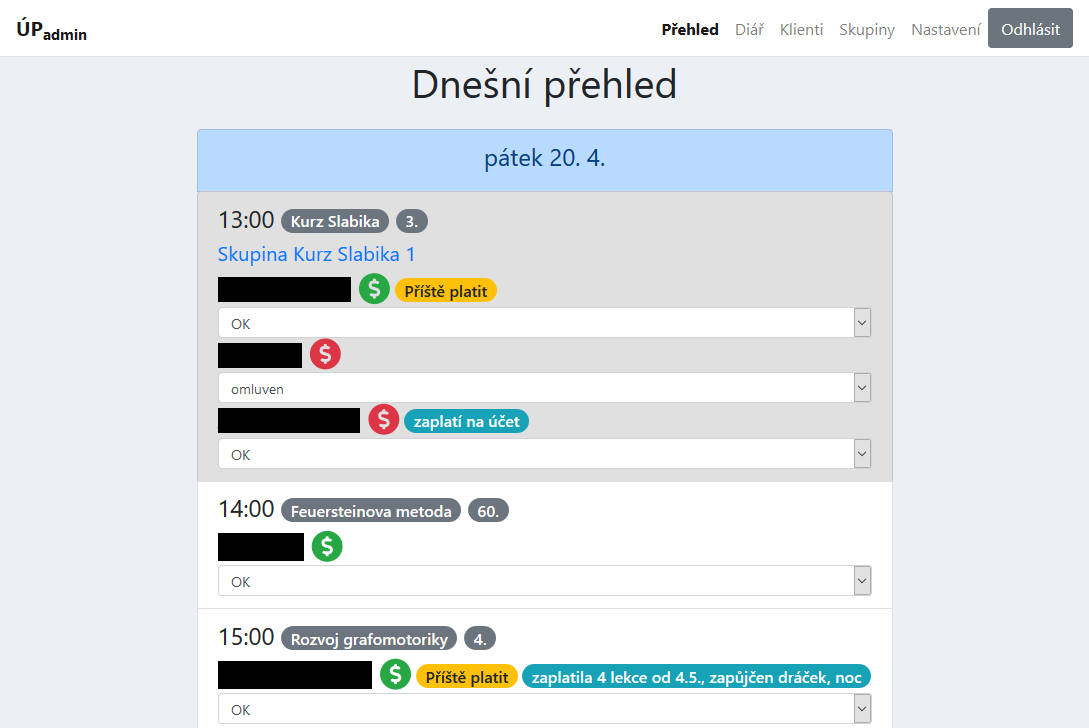
\includegraphics[width=1\textwidth]{img/screen-den.png}
        	\caption{Snímek obrazovky s denním přehledem}\label{fig:screen-den}
        \end{figure}
        
        \begin{figure}\centering
        	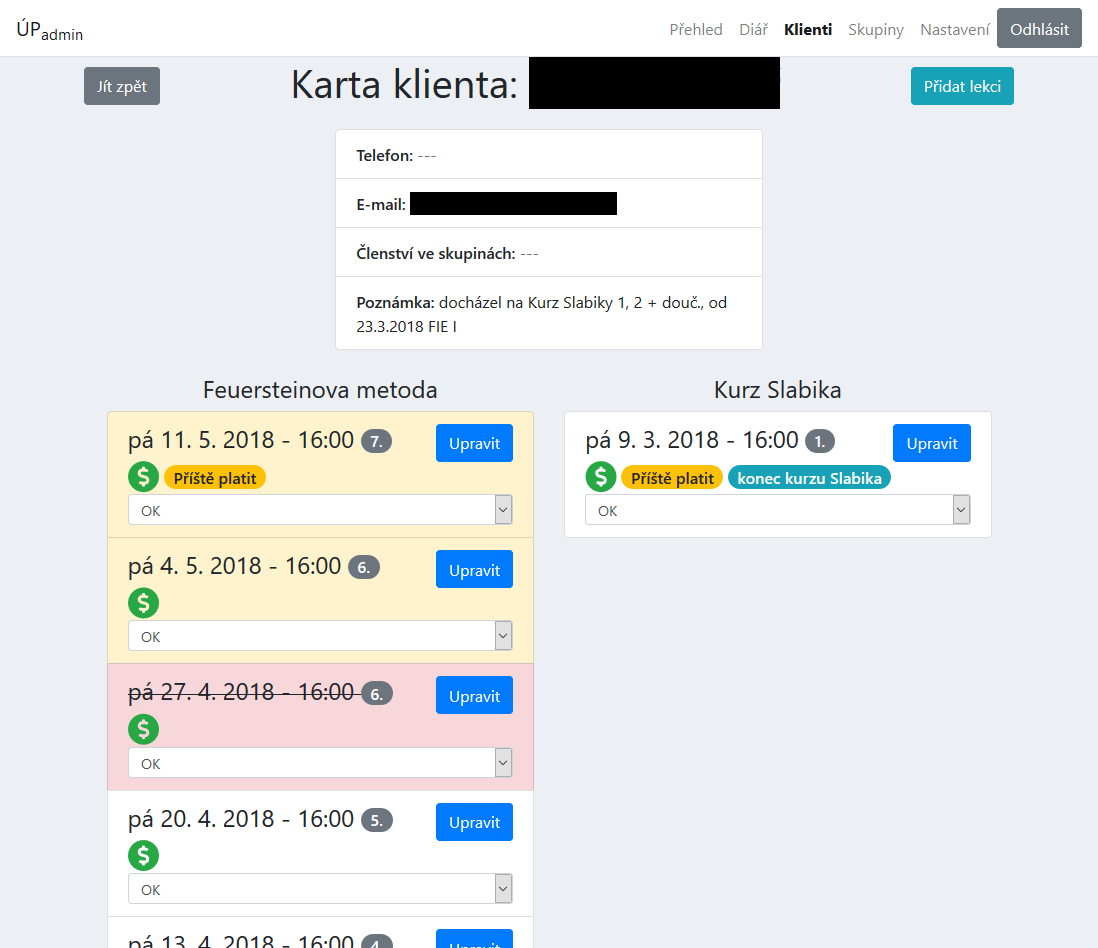
\includegraphics[width=1\textwidth]{img/screen-karta.png}
        	\caption{Snímek obrazovky s kartou klienta}\label{fig:screen-karta}
        \end{figure}
        
        \begin{landscape}
            \begin{figure}\centering
            	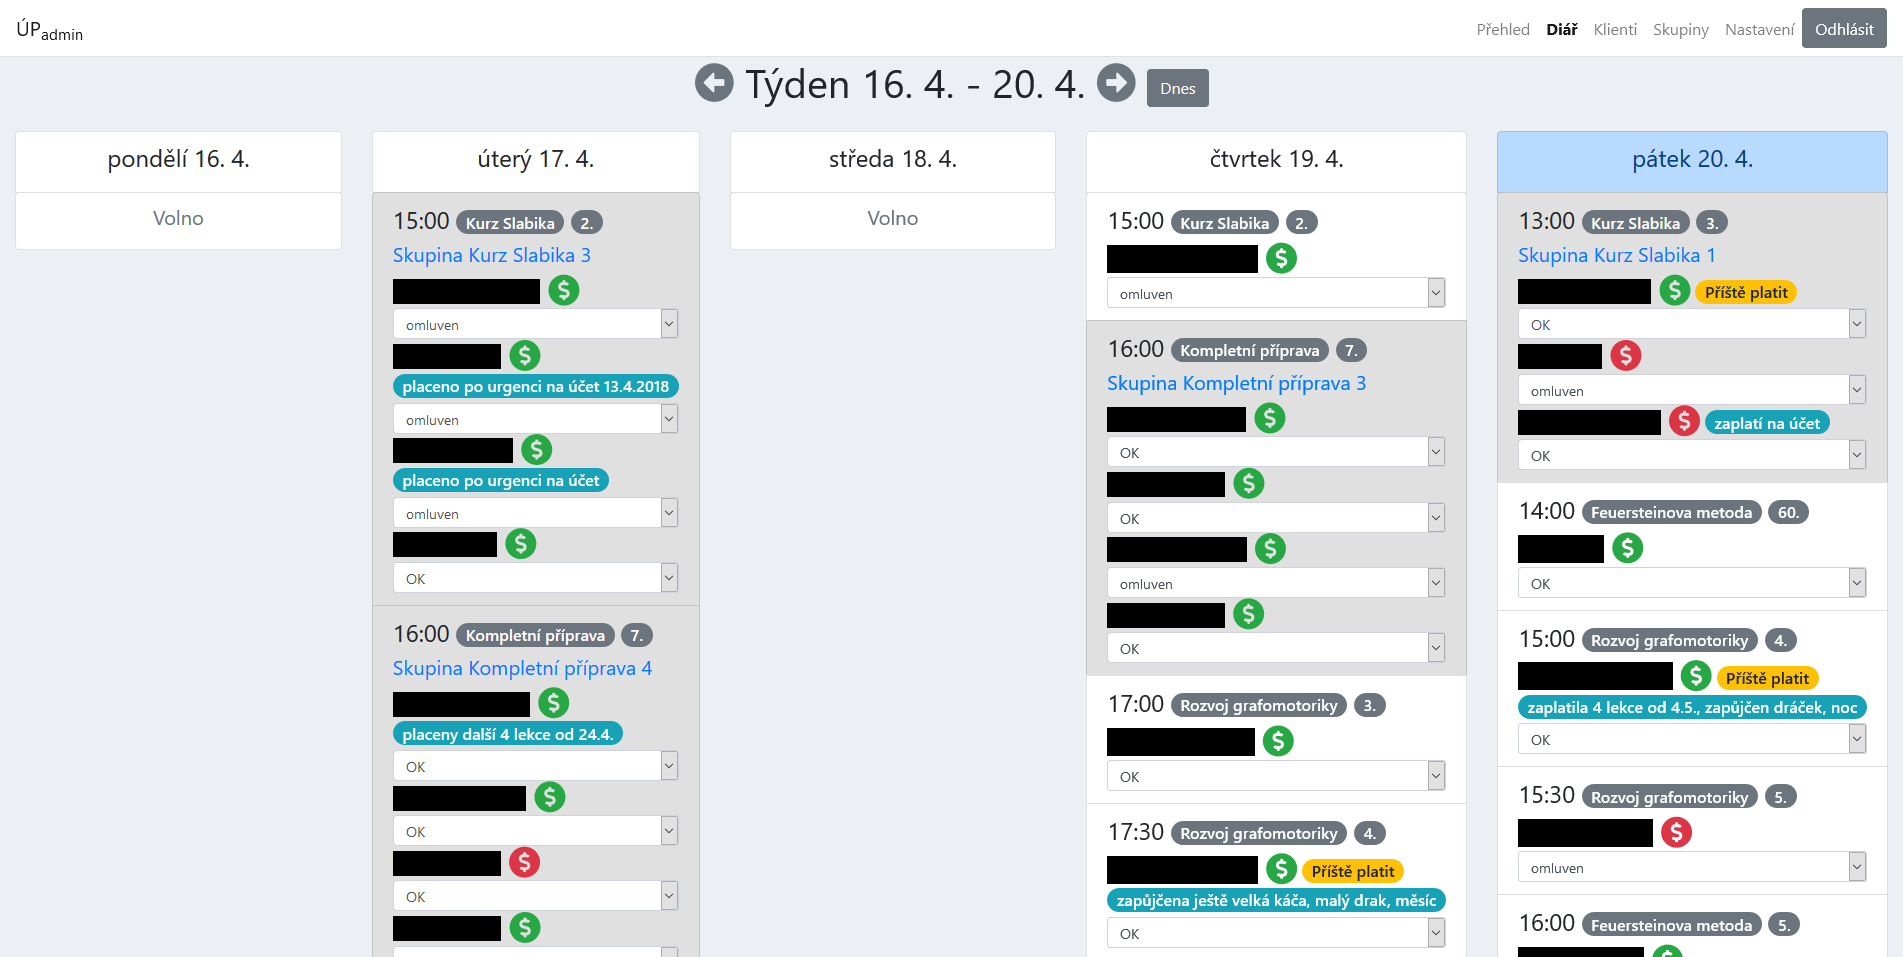
\includegraphics[totalheight=0.8\textheight]{img/screen-tyden.png}
            	\caption{Snímek obrazovky s týdenním přehledem}\label{fig:screen-tyden}
            \end{figure}
        \end{landscape}
\end{document}